% Supplementary material for the new-submission version. All tables are
% generated by scripts/05_make_tables.py and scripts/11_posthoc.py.
\documentclass[10pt,a4paper]{article}
\usepackage[margin=2cm]{geometry}
\usepackage[T1]{fontenc}
\usepackage{amsmath,amssymb}
\usepackage{booktabs,longtable,multirow,makecell}
\usepackage{graphicx}
\usepackage{xcolor}
\usepackage[hidelinks]{hyperref}
\renewcommand{\thetable}{S\arabic{table}}
\renewcommand{\thefigure}{S\arabic{figure}}
\renewcommand{\thesection}{S\arabic{section}}
% AUTO-GENERATED by scripts/05_make_tables.py -- do not edit
\newcommand{\AblAsymBayesCost}{0.825}
\newcommand{\AblAsymBayesPrAuc}{0.517}
\newcommand{\AblAsymBayesRecall}{79.8}
\newcommand{\AblAsymBayesRocAuc}{0.572}
\newcommand{\AblAsymBayesSpec}{32.0}
\newcommand{\AblAsymCostCost}{0.625}
\newcommand{\AblAsymCostPrAuc}{0.517}
\newcommand{\AblAsymCostRecall}{94.8}
\newcommand{\AblAsymCostRocAuc}{0.572}
\newcommand{\AblAsymCostSpec}{8.6}
\newcommand{\AblBalBayesCost}{0.890}
\newcommand{\AblBalBayesPrAuc}{0.486}
\newcommand{\AblBalBayesRecall}{76.6}
\newcommand{\AblBalBayesRocAuc}{0.554}
\newcommand{\AblBalBayesSpec}{33.1}
\newcommand{\AblBalCostCost}{0.660}
\newcommand{\AblBalCostPrAuc}{0.486}
\newcommand{\AblBalCostRecall}{94.3}
\newcommand{\AblBalCostRocAuc}{0.554}
\newcommand{\AblBalCostSpec}{4.3}
\newcommand{\AblDoubleBayesCost}{0.903}
\newcommand{\AblDoubleBayesPrAuc}{0.491}
\newcommand{\AblDoubleBayesRecall}{76.9}
\newcommand{\AblDoubleBayesRocAuc}{0.543}
\newcommand{\AblDoubleBayesSpec}{29.8}
\newcommand{\AblDoubleCostCost}{0.681}
\newcommand{\AblDoubleCostPrAuc}{0.491}
\newcommand{\AblDoubleCostRecall}{93.1}
\newcommand{\AblDoubleCostRocAuc}{0.543}
\newcommand{\AblDoubleCostSpec}{5.3}
\newcommand{\AblDuelBayesCost}{0.890}
\newcommand{\AblDuelBayesPrAuc}{0.494}
\newcommand{\AblDuelBayesRecall}{77.3}
\newcommand{\AblDuelBayesRocAuc}{0.559}
\newcommand{\AblDuelBayesSpec}{30.5}
\newcommand{\AblDuelCostCost}{0.644}
\newcommand{\AblDuelCostPrAuc}{0.494}
\newcommand{\AblDuelCostRecall}{94.6}
\newcommand{\AblDuelCostRocAuc}{0.559}
\newcommand{\AblDuelCostSpec}{5.8}
\newcommand{\AblFullBayesCost}{0.864}
\newcommand{\AblFullBayesPrAuc}{0.500}
\newcommand{\AblFullBayesRecall}{79.2}
\newcommand{\AblFullBayesRocAuc}{0.563}
\newcommand{\AblFullBayesSpec}{27.5}
\newcommand{\AblFullCostCost}{0.667}
\newcommand{\AblFullCostPrAuc}{0.500}
\newcommand{\AblFullCostRecall}{93.7}
\newcommand{\AblFullCostRocAuc}{0.563}
\newcommand{\AblFullCostSpec}{5.4}
\newcommand{\AblGammaZeroBayesCost}{0.825}
\newcommand{\AblGammaZeroBayesPrAuc}{0.510}
\newcommand{\AblGammaZeroBayesRecall}{80.6}
\newcommand{\AblGammaZeroBayesRocAuc}{0.576}
\newcommand{\AblGammaZeroBayesSpec}{29.2}
\newcommand{\AblGammaZeroCostCost}{0.645}
\newcommand{\AblGammaZeroCostPrAuc}{0.510}
\newcommand{\AblGammaZeroCostRecall}{94.4}
\newcommand{\AblGammaZeroCostRocAuc}{0.576}
\newcommand{\AblGammaZeroCostSpec}{6.4}
\newcommand{\AblSoftBayesCost}{0.804}
\newcommand{\AblSoftBayesPrAuc}{0.472}
\newcommand{\AblSoftBayesRecall}{82.9}
\newcommand{\AblSoftBayesRocAuc}{0.529}
\newcommand{\AblSoftBayesSpec}{23.5}
\newcommand{\AblSoftCostCost}{0.634}
\newcommand{\AblSoftCostPrAuc}{0.472}
\newcommand{\AblSoftCostRecall}{94.9}
\newcommand{\AblSoftCostRocAuc}{0.529}
\newcommand{\AblSoftCostSpec}{6.5}
\newcommand{\AblWarmBayesCost}{0.896}
\newcommand{\AblWarmBayesPrAuc}{0.497}
\newcommand{\AblWarmBayesRecall}{77.7}
\newcommand{\AblWarmBayesRocAuc}{0.547}
\newcommand{\AblWarmBayesSpec}{27.7}
\newcommand{\AblWarmCostCost}{0.656}
\newcommand{\AblWarmCostPrAuc}{0.497}
\newcommand{\AblWarmCostRecall}{93.8}
\newcommand{\AblWarmCostRocAuc}{0.547}
\newcommand{\AblWarmCostSpec}{7.1}
\newcommand{\AlwaysAcc}{44.2}
\newcommand{\AlwaysAlarm}{100.0}
\newcommand{\AlwaysBalAcc}{50.0}
\newcommand{\AlwaysCost}{0.558}
\newcommand{\AlwaysFN}{0}
\newcommand{\AlwaysFNR}{0.0}
\newcommand{\AlwaysFP}{5,243}
\newcommand{\AlwaysFPR}{100.0}
\newcommand{\AlwaysFone}{61.3}
\newcommand{\AlwaysGmean}{0.0}
\newcommand{\AlwaysMCC}{0.000}
\newcommand{\AlwaysPrec}{44.2}
\newcommand{\AlwaysRecall}{100.0}
\newcommand{\AlwaysSpec}{0.0}
\newcommand{\AlwaysTN}{0}
\newcommand{\AlwaysTP}{4,147}
\newcommand{\AttAucFracSmall}{87}
\newcommand{\AttAucMaxAbsChange}{0.089}
\newcommand{\AttAucNVariants}{17}
\newcommand{\AttEvasionDropMax}{19}
\newcommand{\AttEvasionDropMin}{4}
\newcommand{\BestBaseline}{RF}
\newcommand{\BestModelAUC}{HGB}
\newcommand{\BestModelCost}{RF}
\newcommand{\CSMLPAttAucMaxDrop}{0.025}
\newcommand{\CSMLPAttAucMaxRise}{0.005}
\newcommand{\CSMLPAttAucaccelspikes}{0.652}
\newcommand{\CSMLPAttAucclean}{0.654}
\newcommand{\CSMLPAttAucfpscap}{0.649}
\newcommand{\CSMLPAttAucrotjitter}{0.654}
\newcommand{\CSMLPAttAucrotsmooth}{0.646}
\newcommand{\CSMLPAttAucspeedscaledown}{0.629}
\newcommand{\CSMLPAttAucspeedscaleup}{0.630}
\newcommand{\CSMLPAttCleanFPR}{93.9}
\newcommand{\CSMLPAttCleanRecall}{99.4}
\newcommand{\CSMLPAttWorstFPR}{100.0}
\newcommand{\CSMLPAttWorstRecall}{95.6}
\newcommand{\CSMLPAttaccelspikesFPR}{99.1}
\newcommand{\CSMLPAttaccelspikesRecall}{99.9}
\newcommand{\CSMLPAttfpscapFPR}{98.3}
\newcommand{\CSMLPAttfpscapRecall}{100.0}
\newcommand{\CSMLPAttrotjitterFPR}{96.5}
\newcommand{\CSMLPAttrotjitterRecall}{99.7}
\newcommand{\CSMLPAttspeedscaleupFPR}{98.2}
\newcommand{\CSMLPAttspeedscaleupRecall}{100.0}
\newcommand{\CSMLPBayesAccEns}{57.4}
\newcommand{\CSMLPBayesAccMean}{57.0}
\newcommand{\CSMLPBayesAccSD}{1.5}
\newcommand{\CSMLPBayesAlarmEns}{73.5}
\newcommand{\CSMLPBayesAlarmMean}{72.1}
\newcommand{\CSMLPBayesAlarmSD}{2.2}
\newcommand{\CSMLPBayesBalAccEns}{60.3}
\newcommand{\CSMLPBayesBalAccMean}{59.7}
\newcommand{\CSMLPBayesBalAccSD}{1.6}
\newcommand{\CSMLPBayesCostEns}{0.691}
\newcommand{\CSMLPBayesCostMean}{0.731}
\newcommand{\CSMLPBayesCostSD}{0.066}
\newcommand{\CSMLPBayesFNEns}{622}
\newcommand{\CSMLPBayesFNMean}{707}
\newcommand{\CSMLPBayesFNREns}{15.0}
\newcommand{\CSMLPBayesFNRMean}{17.0}
\newcommand{\CSMLPBayesFNRSD}{3.1}
\newcommand{\CSMLPBayesFNSD}{129.7}
\newcommand{\CSMLPBayesFPEns}{3,381}
\newcommand{\CSMLPBayesFPMean}{3,332}
\newcommand{\CSMLPBayesFPREns}{64.5}
\newcommand{\CSMLPBayesFPRMean}{63.6}
\newcommand{\CSMLPBayesFPRSD}{2.3}
\newcommand{\CSMLPBayesFPSD}{118.2}
\newcommand{\CSMLPBayesFoneEns}{63.8}
\newcommand{\CSMLPBayesFoneMean}{63.0}
\newcommand{\CSMLPBayesFoneSD}{1.5}
\newcommand{\CSMLPBayesGmeanEns}{54.9}
\newcommand{\CSMLPBayesGmeanMean}{54.9}
\newcommand{\CSMLPBayesGmeanSD}{1.6}
\newcommand{\CSMLPBayesMCCEns}{0.231}
\newcommand{\CSMLPBayesMCCMean}{0.215}
\newcommand{\CSMLPBayesMCCSD}{0.037}
\newcommand{\CSMLPBayesPrAucEns}{0.529}
\newcommand{\CSMLPBayesPrAucMean}{0.521}
\newcommand{\CSMLPBayesPrAucSD}{0.022}
\newcommand{\CSMLPBayesPrecEns}{51.0}
\newcommand{\CSMLPBayesPrecMean}{50.8}
\newcommand{\CSMLPBayesPrecSD}{1.0}
\newcommand{\CSMLPBayesRecallEns}{85.0}
\newcommand{\CSMLPBayesRecallMean}{83.0}
\newcommand{\CSMLPBayesRecallSD}{3.1}
\newcommand{\CSMLPBayesRocAucEns}{0.654}
\newcommand{\CSMLPBayesRocAucMean}{0.644}
\newcommand{\CSMLPBayesRocAucSD}{0.018}
\newcommand{\CSMLPBayesSpecEns}{35.5}
\newcommand{\CSMLPBayesSpecMean}{36.4}
\newcommand{\CSMLPBayesSpecSD}{2.3}
\newcommand{\CSMLPBayesTNEns}{1,862}
\newcommand{\CSMLPBayesTNMean}{1,911}
\newcommand{\CSMLPBayesTNSD}{118.2}
\newcommand{\CSMLPBayesTPEns}{3,525}
\newcommand{\CSMLPBayesTPMean}{3,440}
\newcommand{\CSMLPBayesTPSD}{129.7}
\newcommand{\CSMLPCIBalAccHi}{55.1}
\newcommand{\CSMLPCIBalAccLo}{51.1}
\newcommand{\CSMLPCICostHi}{0.634}
\newcommand{\CSMLPCICostLo}{0.421}
\newcommand{\CSMLPCIMCCHi}{0.218}
\newcommand{\CSMLPCIMCCLo}{0.082}
\newcommand{\CSMLPCIPrAucHi}{0.712}
\newcommand{\CSMLPCIPrAucLo}{0.393}
\newcommand{\CSMLPCIRecallHi}{100.0}
\newcommand{\CSMLPCIRecallLo}{98.5}
\newcommand{\CSMLPCIRocAucHi}{0.781}
\newcommand{\CSMLPCIRocAucLo}{0.527}
\newcommand{\CSMLPCISpecHi}{10.8}
\newcommand{\CSMLPCISpecLo}{2.6}
\newcommand{\CSMLPCostAccEns}{47.3}
\newcommand{\CSMLPCostAccMean}{45.4}
\newcommand{\CSMLPCostAccSD}{0.9}
\newcommand{\CSMLPCostAlarmEns}{96.4}
\newcommand{\CSMLPCostAlarmMean}{98.1}
\newcommand{\CSMLPCostAlarmSD}{1.3}
\newcommand{\CSMLPCostBalAccEns}{52.8}
\newcommand{\CSMLPCostBalAccMean}{51.1}
\newcommand{\CSMLPCostBalAccSD}{0.8}
\newcommand{\CSMLPCostCostEns}{0.537}
\newcommand{\CSMLPCostCostMean}{0.557}
\newcommand{\CSMLPCostCostSD}{0.012}
\newcommand{\CSMLPCostFNEns}{23}
\newcommand{\CSMLPCostFNMean}{27}
\newcommand{\CSMLPCostFNREns}{0.6}
\newcommand{\CSMLPCostFNRMean}{0.6}
\newcommand{\CSMLPCostFNRSD}{0.7}
\newcommand{\CSMLPCostFNSD}{28.4}
\newcommand{\CSMLPCostFPEns}{4,925}
\newcommand{\CSMLPCostFPMean}{5,096}
\newcommand{\CSMLPCostFPREns}{93.9}
\newcommand{\CSMLPCostFPRMean}{97.2}
\newcommand{\CSMLPCostFPRSD}{1.9}
\newcommand{\CSMLPCostFPSD}{100.6}
\newcommand{\CSMLPCostFoneEns}{62.5}
\newcommand{\CSMLPCostFoneMean}{61.7}
\newcommand{\CSMLPCostFoneSD}{0.4}
\newcommand{\CSMLPCostGmeanEns}{24.6}
\newcommand{\CSMLPCostGmeanMean}{14.7}
\newcommand{\CSMLPCostGmeanSD}{8.8}
\newcommand{\CSMLPCostMCCEns}{0.146}
\newcommand{\CSMLPCostMCCMean}{0.072}
\newcommand{\CSMLPCostMCCSD}{0.049}
\newcommand{\CSMLPCostPrAucEns}{0.529}
\newcommand{\CSMLPCostPrAucMean}{0.521}
\newcommand{\CSMLPCostPrAucSD}{0.022}
\newcommand{\CSMLPCostPrecEns}{45.6}
\newcommand{\CSMLPCostPrecMean}{44.7}
\newcommand{\CSMLPCostPrecSD}{0.4}
\newcommand{\CSMLPCostRecallEns}{99.4}
\newcommand{\CSMLPCostRecallMean}{99.4}
\newcommand{\CSMLPCostRecallSD}{0.7}
\newcommand{\CSMLPCostRocAucEns}{0.654}
\newcommand{\CSMLPCostRocAucMean}{0.644}
\newcommand{\CSMLPCostRocAucSD}{0.018}
\newcommand{\CSMLPCostSpecEns}{6.1}
\newcommand{\CSMLPCostSpecMean}{2.8}
\newcommand{\CSMLPCostSpecSD}{1.9}
\newcommand{\CSMLPCostTNEns}{318}
\newcommand{\CSMLPCostTNMean}{147}
\newcommand{\CSMLPCostTNSD}{100.6}
\newcommand{\CSMLPCostTPEns}{4,124}
\newcommand{\CSMLPCostTPMean}{4,120}
\newcommand{\CSMLPCostTPSD}{28.4}
\newcommand{\CSMLPEvDelay}{0}
\newcommand{\CSMLPEvDetected}{26}
\newcommand{\CSMLPEvFreeAlarm}{88.1}
\newcommand{\CSMLPEvPreAlarm}{92.9}
\newcommand{\CSMLPMeanSeconds}{3}
\newcommand{\CSMLPMedBestEpoch}{14}
\newcommand{\CSMLPOptGap}{+0.033}
\newcommand{\CSMLPOptInner}{0.501}
\newcommand{\CSMLPQAbsMax}{nan}
\newcommand{\CSMLPRecAccEns}{51.4}
\newcommand{\CSMLPRecAccMean}{48.6}
\newcommand{\CSMLPRecAccSD}{2.1}
\newcommand{\CSMLPRecAlarmEns}{90.6}
\newcommand{\CSMLPRecAlarmMean}{94.0}
\newcommand{\CSMLPRecAlarmSD}{2.6}
\newcommand{\CSMLPRecBalAccEns}{56.2}
\newcommand{\CSMLPRecBalAccMean}{53.8}
\newcommand{\CSMLPRecBalAccSD}{1.9}
\newcommand{\CSMLPRecCostEns}{0.531}
\newcommand{\CSMLPRecCostMean}{0.544}
\newcommand{\CSMLPRecCostSD}{0.025}
\newcommand{\CSMLPRecFNEns}{105}
\newcommand{\CSMLPRecFNMean}{72}
\newcommand{\CSMLPRecFNREns}{2.5}
\newcommand{\CSMLPRecFNRMean}{1.7}
\newcommand{\CSMLPRecFNRSD}{1.2}
\newcommand{\CSMLPRecFNSD}{48.0}
\newcommand{\CSMLPRecFPEns}{4,463}
\newcommand{\CSMLPRecFPMean}{4,753}
\newcommand{\CSMLPRecFPREns}{85.1}
\newcommand{\CSMLPRecFPRMean}{90.7}
\newcommand{\CSMLPRecFPRSD}{4.2}
\newcommand{\CSMLPRecFPSD}{218.6}
\newcommand{\CSMLPRecFoneEns}{63.9}
\newcommand{\CSMLPRecFoneMean}{62.8}
\newcommand{\CSMLPRecFoneSD}{0.9}
\newcommand{\CSMLPRecGmeanEns}{38.1}
\newcommand{\CSMLPRecGmeanMean}{29.4}
\newcommand{\CSMLPRecGmeanSD}{8.0}
\newcommand{\CSMLPRecMCCEns}{0.210}
\newcommand{\CSMLPRecMCCMean}{0.156}
\newcommand{\CSMLPRecMCCSD}{0.052}
\newcommand{\CSMLPRecPrAucEns}{0.529}
\newcommand{\CSMLPRecPrAucMean}{0.521}
\newcommand{\CSMLPRecPrAucSD}{0.022}
\newcommand{\CSMLPRecPrecEns}{47.5}
\newcommand{\CSMLPRecPrecMean}{46.2}
\newcommand{\CSMLPRecPrecSD}{1.0}
\newcommand{\CSMLPRecRecallEns}{97.5}
\newcommand{\CSMLPRecRecallMean}{98.3}
\newcommand{\CSMLPRecRecallSD}{1.2}
\newcommand{\CSMLPRecRocAucEns}{0.654}
\newcommand{\CSMLPRecRocAucMean}{0.644}
\newcommand{\CSMLPRecRocAucSD}{0.018}
\newcommand{\CSMLPRecSpecEns}{14.9}
\newcommand{\CSMLPRecSpecMean}{9.3}
\newcommand{\CSMLPRecSpecSD}{4.2}
\newcommand{\CSMLPRecTNEns}{780}
\newcommand{\CSMLPRecTNMean}{490}
\newcommand{\CSMLPRecTNSD}{218.6}
\newcommand{\CSMLPRecTPEns}{4,042}
\newcommand{\CSMLPRecTPMean}{4,075}
\newcommand{\CSMLPRecTPSD}{48.0}
\newcommand{\CSMLPRocFPRatEightZero}{56.7}
\newcommand{\CSMLPRocFPRatNineFive}{84.4}
\newcommand{\CSMLPRocFPRatNineNine}{93.6}
\newcommand{\CSMLPRocFPRatNineZero}{75.9}
\newcommand{\CSMLPnProfile}{2}
\newcommand{\DOneFPRMax}{97}
\newcommand{\DOneFPRMin}{82}
\newcommand{\DQNAttAucMaxDrop}{0.064}
\newcommand{\DQNAttAucMaxRise}{0.035}
\newcommand{\DQNAttAucaccelspikes}{0.605}
\newcommand{\DQNAttAucclean}{0.665}
\newcommand{\DQNAttAucfpscap}{0.665}
\newcommand{\DQNAttAucrotjitter}{0.677}
\newcommand{\DQNAttAucrotsmooth}{0.676}
\newcommand{\DQNAttAucspeedscaledown}{0.632}
\newcommand{\DQNAttAucspeedscaleup}{0.680}
\newcommand{\DQNAttCleanFPR}{83.7}
\newcommand{\DQNAttCleanRecall}{96.9}
\newcommand{\DQNAttWorstFPR}{97.5}
\newcommand{\DQNAttWorstRecall}{87.3}
\newcommand{\DQNAttaccelspikesFPR}{95.4}
\newcommand{\DQNAttaccelspikesRecall}{97.9}
\newcommand{\DQNAttfpscapFPR}{83.7}
\newcommand{\DQNAttfpscapRecall}{96.9}
\newcommand{\DQNAttrotjitterFPR}{83.5}
\newcommand{\DQNAttrotjitterRecall}{94.8}
\newcommand{\DQNAttspeedscaleupFPR}{91.8}
\newcommand{\DQNAttspeedscaleupRecall}{97.8}
\newcommand{\DQNBayesAccEns}{58.6}
\newcommand{\DQNBayesAccMean}{58.3}
\newcommand{\DQNBayesAccSD}{1.0}
\newcommand{\DQNBayesAlarmEns}{73.7}
\newcommand{\DQNBayesAlarmMean}{72.7}
\newcommand{\DQNBayesAlarmSD}{1.2}
\newcommand{\DQNBayesBalAccEns}{61.5}
\newcommand{\DQNBayesBalAccMean}{61.1}
\newcommand{\DQNBayesBalAccSD}{1.0}
\newcommand{\DQNBayesCostEns}{0.653}
\newcommand{\DQNBayesCostMean}{0.680}
\newcommand{\DQNBayesCostSD}{0.035}
\newcommand{\DQNBayesFNEns}{561}
\newcommand{\DQNBayesFNMean}{617}
\newcommand{\DQNBayesFNREns}{13.5}
\newcommand{\DQNBayesFNRMean}{14.9}
\newcommand{\DQNBayesFNRSD}{1.7}
\newcommand{\DQNBayesFNSD}{68.5}
\newcommand{\DQNBayesFPEns}{3,330}
\newcommand{\DQNBayesFPMean}{3,297}
\newcommand{\DQNBayesFPREns}{63.5}
\newcommand{\DQNBayesFPRMean}{62.9}
\newcommand{\DQNBayesFPRSD}{1.5}
\newcommand{\DQNBayesFPSD}{78.6}
\newcommand{\DQNBayesFoneEns}{64.8}
\newcommand{\DQNBayesFoneMean}{64.3}
\newcommand{\DQNBayesFoneSD}{0.9}
\newcommand{\DQNBayesGmeanEns}{56.2}
\newcommand{\DQNBayesGmeanMean}{56.2}
\newcommand{\DQNBayesGmeanSD}{1.1}
\newcommand{\DQNBayesMCCEns}{0.259}
\newcommand{\DQNBayesMCCMean}{0.248}
\newcommand{\DQNBayesMCCSD}{0.022}
\newcommand{\DQNBayesPrAucEns}{0.606}
\newcommand{\DQNBayesPrAucMean}{0.595}
\newcommand{\DQNBayesPrAucSD}{0.022}
\newcommand{\DQNBayesPrecEns}{51.9}
\newcommand{\DQNBayesPrecMean}{51.7}
\newcommand{\DQNBayesPrecSD}{0.7}
\newcommand{\DQNBayesRecallEns}{86.5}
\newcommand{\DQNBayesRecallMean}{85.1}
\newcommand{\DQNBayesRecallSD}{1.7}
\newcommand{\DQNBayesRocAucEns}{0.665}
\newcommand{\DQNBayesRocAucMean}{0.661}
\newcommand{\DQNBayesRocAucSD}{0.013}
\newcommand{\DQNBayesSpecEns}{36.5}
\newcommand{\DQNBayesSpecMean}{37.1}
\newcommand{\DQNBayesSpecSD}{1.5}
\newcommand{\DQNBayesTNEns}{1,913}
\newcommand{\DQNBayesTNMean}{1,946}
\newcommand{\DQNBayesTNSD}{78.6}
\newcommand{\DQNBayesTPEns}{3,586}
\newcommand{\DQNBayesTPMean}{3,530}
\newcommand{\DQNBayesTPSD}{68.5}
\newcommand{\DQNCIBalAccHi}{61.1}
\newcommand{\DQNCIBalAccLo}{53.0}
\newcommand{\DQNCICostHi}{0.654}
\newcommand{\DQNCICostLo}{0.417}
\newcommand{\DQNCIMCCHi}{0.319}
\newcommand{\DQNCIMCCLo}{0.110}
\newcommand{\DQNCIPrAucHi}{0.778}
\newcommand{\DQNCIPrAucLo}{0.456}
\newcommand{\DQNCIRecallHi}{99.7}
\newcommand{\DQNCIRecallLo}{92.6}
\newcommand{\DQNCIRocAucHi}{0.785}
\newcommand{\DQNCIRocAucLo}{0.558}
\newcommand{\DQNCISpecHi}{24.8}
\newcommand{\DQNCISpecLo}{8.7}
\newcommand{\DQNCostAccEns}{51.9}
\newcommand{\DQNCostAccMean}{50.1}
\newcommand{\DQNCostAccSD}{1.9}
\newcommand{\DQNCostAlarmEns}{89.6}
\newcommand{\DQNCostAlarmMean}{89.8}
\newcommand{\DQNCostAlarmSD}{3.7}
\newcommand{\DQNCostBalAccEns}{56.6}
\newcommand{\DQNCostBalAccMean}{54.8}
\newcommand{\DQNCostBalAccSD}{1.6}
\newcommand{\DQNCostCostEns}{0.536}
\newcommand{\DQNCostCostMean}{0.584}
\newcommand{\DQNCostCostSD}{0.040}
\newcommand{\DQNCostFNEns}{129}
\newcommand{\DQNCostFNMean}{200}
\newcommand{\DQNCostFNREns}{3.1}
\newcommand{\DQNCostFNRMean}{4.8}
\newcommand{\DQNCostFNRSD}{2.7}
\newcommand{\DQNCostFNSD}{109.9}
\newcommand{\DQNCostFPEns}{4,391}
\newcommand{\DQNCostFPMean}{4,485}
\newcommand{\DQNCostFPREns}{83.7}
\newcommand{\DQNCostFPRMean}{85.5}
\newcommand{\DQNCostFPRSD}{4.9}
\newcommand{\DQNCostFPSD}{254.4}
\newcommand{\DQNCostFoneEns}{64.0}
\newcommand{\DQNCostFoneMean}{62.8}
\newcommand{\DQNCostFoneSD}{0.8}
\newcommand{\DQNCostGmeanEns}{39.7}
\newcommand{\DQNCostGmeanMean}{36.6}
\newcommand{\DQNCostGmeanSD}{5.8}
\newcommand{\DQNCostMCCEns}{0.213}
\newcommand{\DQNCostMCCMean}{0.158}
\newcommand{\DQNCostMCCSD}{0.038}
\newcommand{\DQNCostPrAucEns}{0.606}
\newcommand{\DQNCostPrAucMean}{0.595}
\newcommand{\DQNCostPrAucSD}{0.022}
\newcommand{\DQNCostPrecEns}{47.8}
\newcommand{\DQNCostPrecMean}{46.8}
\newcommand{\DQNCostPrecSD}{1.0}
\newcommand{\DQNCostRecallEns}{96.9}
\newcommand{\DQNCostRecallMean}{95.2}
\newcommand{\DQNCostRecallSD}{2.7}
\newcommand{\DQNCostRocAucEns}{0.665}
\newcommand{\DQNCostRocAucMean}{0.661}
\newcommand{\DQNCostRocAucSD}{0.013}
\newcommand{\DQNCostSpecEns}{16.3}
\newcommand{\DQNCostSpecMean}{14.5}
\newcommand{\DQNCostSpecSD}{4.9}
\newcommand{\DQNCostTNEns}{852}
\newcommand{\DQNCostTNMean}{758}
\newcommand{\DQNCostTNSD}{254.4}
\newcommand{\DQNCostTPEns}{4,018}
\newcommand{\DQNCostTPMean}{3,947}
\newcommand{\DQNCostTPSD}{109.9}
\newcommand{\DQNEvDelay}{0}
\newcommand{\DQNEvDetected}{25}
\newcommand{\DQNEvFreeAlarm}{70.4}
\newcommand{\DQNEvPreAlarm}{77.4}
\newcommand{\DQNGammas}{0, 0.9, 0.9, 0.9, 0}
\newcommand{\DQNMeanSeconds}{18}
\newcommand{\DQNMedBestEpoch}{8}
\newcommand{\DQNOptGap}{+0.065}
\newcommand{\DQNOptInner}{0.478}
\newcommand{\DQNOverest}{+0.393}
\newcommand{\DQNQAbsMax}{10.10}
\newcommand{\DQNRecAccEns}{55.8}
\newcommand{\DQNRecAccMean}{54.1}
\newcommand{\DQNRecAccSD}{1.3}
\newcommand{\DQNRecAlarmEns}{81.1}
\newcommand{\DQNRecAlarmMean}{84.3}
\newcommand{\DQNRecAlarmSD}{3.0}
\newcommand{\DQNRecBalAccEns}{59.5}
\newcommand{\DQNRecBalAccMean}{58.3}
\newcommand{\DQNRecBalAccSD}{1.2}
\newcommand{\DQNRecCostEns}{0.588}
\newcommand{\DQNRecCostMean}{0.573}
\newcommand{\DQNRecCostSD}{0.052}
\newcommand{\DQNRecFNEns}{343}
\newcommand{\DQNRecFNMean}{268}
\newcommand{\DQNRecFNREns}{8.3}
\newcommand{\DQNRecFNRMean}{6.5}
\newcommand{\DQNRecFNRSD}{2.9}
\newcommand{\DQNRecFNSD}{120.8}
\newcommand{\DQNRecFPEns}{3,810}
\newcommand{\DQNRecFPMean}{4,038}
\newcommand{\DQNRecFPREns}{72.7}
\newcommand{\DQNRecFPRMean}{77.0}
\newcommand{\DQNRecFPRSD}{3.4}
\newcommand{\DQNRecFPSD}{179.9}
\newcommand{\DQNRecFoneEns}{64.7}
\newcommand{\DQNRecFoneMean}{64.3}
\newcommand{\DQNRecFoneSD}{1.0}
\newcommand{\DQNRecGmeanEns}{50.1}
\newcommand{\DQNRecGmeanMean}{46.2}
\newcommand{\DQNRecGmeanSD}{3.0}
\newcommand{\DQNRecMCCEns}{0.242}
\newcommand{\DQNRecMCCMean}{0.227}
\newcommand{\DQNRecMCCSD}{0.032}
\newcommand{\DQNRecPrAucEns}{0.606}
\newcommand{\DQNRecPrAucMean}{0.595}
\newcommand{\DQNRecPrAucSD}{0.022}
\newcommand{\DQNRecPrecEns}{50.0}
\newcommand{\DQNRecPrecMean}{49.0}
\newcommand{\DQNRecPrecSD}{0.8}
\newcommand{\DQNRecRecallEns}{91.7}
\newcommand{\DQNRecRecallMean}{93.5}
\newcommand{\DQNRecRecallSD}{2.9}
\newcommand{\DQNRecRocAucEns}{0.665}
\newcommand{\DQNRecRocAucMean}{0.661}
\newcommand{\DQNRecRocAucSD}{0.013}
\newcommand{\DQNRecSpecEns}{27.3}
\newcommand{\DQNRecSpecMean}{23.0}
\newcommand{\DQNRecSpecSD}{3.4}
\newcommand{\DQNRecTNEns}{1,433}
\newcommand{\DQNRecTNMean}{1,205}
\newcommand{\DQNRecTNSD}{179.9}
\newcommand{\DQNRecTPEns}{3,804}
\newcommand{\DQNRecTPMean}{3,879}
\newcommand{\DQNRecTPSD}{120.8}
\newcommand{\DQNRocFPRatEightZero}{49.3}
\newcommand{\DQNRocFPRatNineFive}{82.4}
\newcommand{\DQNRocFPRatNineNine}{99.8}
\newcommand{\DQNRocFPRatNineZero}{76.5}
\newcommand{\DQNnProfile}{2}
\newcommand{\ECBAttAucMaxDrop}{0.089}
\newcommand{\ECBAttAucMaxRise}{0.052}
\newcommand{\ECBAttAucaccelspikes}{0.575}
\newcommand{\ECBAttAucclean}{0.659}
\newcommand{\ECBAttAucfpscap}{0.659}
\newcommand{\ECBAttAucrotjitter}{0.682}
\newcommand{\ECBAttAucrotsmooth}{0.658}
\newcommand{\ECBAttAucspeedscaledown}{0.648}
\newcommand{\ECBAttAucspeedscaleup}{0.648}
\newcommand{\ECBAttCleanFPR}{85.4}
\newcommand{\ECBAttCleanRecall}{96.6}
\newcommand{\ECBAttWorstFPR}{98.9}
\newcommand{\ECBAttWorstRecall}{78.0}
\newcommand{\ECBAttaccelspikesFPR}{97.7}
\newcommand{\ECBAttaccelspikesRecall}{99.3}
\newcommand{\ECBAttfpscapFPR}{85.4}
\newcommand{\ECBAttfpscapRecall}{96.6}
\newcommand{\ECBAttrotjitterFPR}{88.2}
\newcommand{\ECBAttrotjitterRecall}{96.1}
\newcommand{\ECBAttspeedscaleupFPR}{95.9}
\newcommand{\ECBAttspeedscaleupRecall}{98.7}
\newcommand{\ECBBayesAccEns}{58.6}
\newcommand{\ECBBayesAccMean}{58.7}
\newcommand{\ECBBayesAccSD}{1.6}
\newcommand{\ECBBayesAlarmEns}{72.2}
\newcommand{\ECBBayesAlarmMean}{73.0}
\newcommand{\ECBBayesAlarmSD}{2.3}
\newcommand{\ECBBayesBalAccEns}{61.3}
\newcommand{\ECBBayesBalAccMean}{61.5}
\newcommand{\ECBBayesBalAccSD}{1.5}
\newcommand{\ECBBayesCostEns}{0.681}
\newcommand{\ECBBayesCostMean}{0.663}
\newcommand{\ECBBayesCostSD}{0.044}
\newcommand{\ECBBayesFNEns}{627}
\newcommand{\ECBBayesFNMean}{587}
\newcommand{\ECBBayesFNREns}{15.1}
\newcommand{\ECBBayesFNRMean}{14.1}
\newcommand{\ECBBayesFNRSD}{2.2}
\newcommand{\ECBBayesFNSD}{90.3}
\newcommand{\ECBBayesFPEns}{3,262}
\newcommand{\ECBBayesFPMean}{3,291}
\newcommand{\ECBBayesFPREns}{62.2}
\newcommand{\ECBBayesFPRMean}{62.8}
\newcommand{\ECBBayesFPRSD}{3.0}
\newcommand{\ECBBayesFPSD}{159.4}
\newcommand{\ECBBayesFoneEns}{64.4}
\newcommand{\ECBBayesFoneMean}{64.7}
\newcommand{\ECBBayesFoneSD}{1.1}
\newcommand{\ECBBayesGmeanEns}{56.6}
\newcommand{\ECBBayesGmeanMean}{56.5}
\newcommand{\ECBBayesGmeanSD}{2.2}
\newcommand{\ECBBayesMCCEns}{0.251}
\newcommand{\ECBBayesMCCMean}{0.258}
\newcommand{\ECBBayesMCCSD}{0.031}
\newcommand{\ECBBayesPrAucEns}{0.565}
\newcommand{\ECBBayesPrAucMean}{0.562}
\newcommand{\ECBBayesPrAucSD}{0.006}
\newcommand{\ECBBayesPrecEns}{51.9}
\newcommand{\ECBBayesPrecMean}{52.0}
\newcommand{\ECBBayesPrecSD}{1.1}
\newcommand{\ECBBayesRecallEns}{84.9}
\newcommand{\ECBBayesRecallMean}{85.9}
\newcommand{\ECBBayesRecallSD}{2.2}
\newcommand{\ECBBayesRocAucEns}{0.659}
\newcommand{\ECBBayesRocAucMean}{0.653}
\newcommand{\ECBBayesRocAucSD}{0.011}
\newcommand{\ECBBayesSpecEns}{37.8}
\newcommand{\ECBBayesSpecMean}{37.2}
\newcommand{\ECBBayesSpecSD}{3.0}
\newcommand{\ECBBayesTNEns}{1,981}
\newcommand{\ECBBayesTNMean}{1,952}
\newcommand{\ECBBayesTNSD}{159.4}
\newcommand{\ECBBayesTPEns}{3,520}
\newcommand{\ECBBayesTPMean}{3,560}
\newcommand{\ECBBayesTPSD}{90.3}
\newcommand{\ECBCIBalAccHi}{59.6}
\newcommand{\ECBCIBalAccLo}{51.7}
\newcommand{\ECBCICostHi}{0.673}
\newcommand{\ECBCICostLo}{0.431}
\newcommand{\ECBCIMCCHi}{0.291}
\newcommand{\ECBCIMCCLo}{0.063}
\newcommand{\ECBCIPrAucHi}{0.740}
\newcommand{\ECBCIPrAucLo}{0.429}
\newcommand{\ECBCIRecallHi}{99.6}
\newcommand{\ECBCIRecallLo}{92.2}
\newcommand{\ECBCIRocAucHi}{0.767}
\newcommand{\ECBCIRocAucLo}{0.550}
\newcommand{\ECBCISpecHi}{21.4}
\newcommand{\ECBCISpecLo}{8.3}
\newcommand{\ECBCostAccEns}{50.8}
\newcommand{\ECBCostAccMean}{47.6}
\newcommand{\ECBCostAccSD}{1.2}
\newcommand{\ECBCostAlarmEns}{90.4}
\newcommand{\ECBCostAlarmMean}{94.0}
\newcommand{\ECBCostAlarmSD}{2.6}
\newcommand{\ECBCostBalAccEns}{55.6}
\newcommand{\ECBCostBalAccMean}{52.8}
\newcommand{\ECBCostBalAccSD}{1.2}
\newcommand{\ECBCostCostEns}{0.552}
\newcommand{\ECBCostCostMean}{0.575}
\newcommand{\ECBCostCostSD}{0.055}
\newcommand{\ECBCostFNEns}{140}
\newcommand{\ECBCostFNMean}{120}
\newcommand{\ECBCostFNREns}{3.4}
\newcommand{\ECBCostFNRMean}{2.9}
\newcommand{\ECBCostFNRSD}{2.9}
\newcommand{\ECBCostFNSD}{119.7}
\newcommand{\ECBCostFPEns}{4,480}
\newcommand{\ECBCostFPMean}{4,801}
\newcommand{\ECBCostFPREns}{85.4}
\newcommand{\ECBCostFPRMean}{91.6}
\newcommand{\ECBCostFPRSD}{2.8}
\newcommand{\ECBCostFPSD}{147.1}
\newcommand{\ECBCostFoneEns}{63.4}
\newcommand{\ECBCostFoneMean}{62.1}
\newcommand{\ECBCostFoneSD}{1.0}
\newcommand{\ECBCostGmeanEns}{37.5}
\newcommand{\ECBCostGmeanMean}{28.2}
\newcommand{\ECBCostGmeanSD}{5.0}
\newcommand{\ECBCostMCCEns}{0.188}
\newcommand{\ECBCostMCCMean}{0.122}
\newcommand{\ECBCostMCCSD}{0.052}
\newcommand{\ECBCostPrAucEns}{0.565}
\newcommand{\ECBCostPrAucMean}{0.562}
\newcommand{\ECBCostPrAucSD}{0.006}
\newcommand{\ECBCostPrecEns}{47.2}
\newcommand{\ECBCostPrecMean}{45.6}
\newcommand{\ECBCostPrecSD}{0.6}
\newcommand{\ECBCostRecallEns}{96.6}
\newcommand{\ECBCostRecallMean}{97.1}
\newcommand{\ECBCostRecallSD}{2.9}
\newcommand{\ECBCostRocAucEns}{0.659}
\newcommand{\ECBCostRocAucMean}{0.653}
\newcommand{\ECBCostRocAucSD}{0.011}
\newcommand{\ECBCostSpecEns}{14.6}
\newcommand{\ECBCostSpecMean}{8.4}
\newcommand{\ECBCostSpecSD}{2.8}
\newcommand{\ECBCostTNEns}{763}
\newcommand{\ECBCostTNMean}{442}
\newcommand{\ECBCostTNSD}{147.1}
\newcommand{\ECBCostTPEns}{4,007}
\newcommand{\ECBCostTPMean}{4,027}
\newcommand{\ECBCostTPSD}{119.7}
\newcommand{\ECBEvDelay}{0}
\newcommand{\ECBEvDetected}{25}
\newcommand{\ECBEvFreeAlarm}{76.9}
\newcommand{\ECBEvPreAlarm}{73.1}
\newcommand{\ECBMeanSeconds}{36}
\newcommand{\ECBMedBestEpoch}{8}
\newcommand{\ECBOptGap}{+0.070}
\newcommand{\ECBOptInner}{0.488}
\newcommand{\ECBOverest}{+0.088}
\newcommand{\ECBQAbsMax}{0.95}
\newcommand{\ECBRecAccEns}{53.0}
\newcommand{\ECBRecAccMean}{50.4}
\newcommand{\ECBRecAccSD}{1.5}
\newcommand{\ECBRecAlarmEns}{84.4}
\newcommand{\ECBRecAlarmMean}{89.5}
\newcommand{\ECBRecAlarmSD}{2.7}
\newcommand{\ECBRecBalAccEns}{57.1}
\newcommand{\ECBRecBalAccMean}{55.1}
\newcommand{\ECBRecBalAccSD}{1.4}
\newcommand{\ECBRecCostEns}{0.605}
\newcommand{\ECBRecCostMean}{0.581}
\newcommand{\ECBRecCostSD}{0.051}
\newcommand{\ECBRecFNEns}{317}
\newcommand{\ECBRecFNMean}{200}
\newcommand{\ECBRecFNREns}{7.6}
\newcommand{\ECBRecFNRMean}{4.8}
\newcommand{\ECBRecFNRSD}{2.7}
\newcommand{\ECBRecFNSD}{110.7}
\newcommand{\ECBRecFPEns}{4,093}
\newcommand{\ECBRecFPMean}{4,456}
\newcommand{\ECBRecFPREns}{78.1}
\newcommand{\ECBRecFPRMean}{85.0}
\newcommand{\ECBRecFPRSD}{3.3}
\newcommand{\ECBRecFPSD}{170.4}
\newcommand{\ECBRecFoneEns}{63.5}
\newcommand{\ECBRecFoneMean}{62.9}
\newcommand{\ECBRecFoneSD}{1.0}
\newcommand{\ECBRecGmeanEns}{45.0}
\newcommand{\ECBRecGmeanMean}{37.6}
\newcommand{\ECBRecGmeanSD}{4.2}
\newcommand{\ECBRecMCCEns}{0.195}
\newcommand{\ECBRecMCCMean}{0.167}
\newcommand{\ECBRecMCCSD}{0.042}
\newcommand{\ECBRecPrAucEns}{0.565}
\newcommand{\ECBRecPrAucMean}{0.562}
\newcommand{\ECBRecPrAucSD}{0.006}
\newcommand{\ECBRecPrecEns}{48.3}
\newcommand{\ECBRecPrecMean}{47.0}
\newcommand{\ECBRecPrecSD}{0.8}
\newcommand{\ECBRecRecallEns}{92.4}
\newcommand{\ECBRecRecallMean}{95.2}
\newcommand{\ECBRecRecallSD}{2.7}
\newcommand{\ECBRecRocAucEns}{0.659}
\newcommand{\ECBRecRocAucMean}{0.653}
\newcommand{\ECBRecRocAucSD}{0.011}
\newcommand{\ECBRecSpecEns}{21.9}
\newcommand{\ECBRecSpecMean}{15.0}
\newcommand{\ECBRecSpecSD}{3.3}
\newcommand{\ECBRecTNEns}{1,150}
\newcommand{\ECBRecTNMean}{787}
\newcommand{\ECBRecTNSD}{170.4}
\newcommand{\ECBRecTPEns}{3,830}
\newcommand{\ECBRecTPMean}{3,947}
\newcommand{\ECBRecTPSD}{110.7}
\newcommand{\ECBRocFPRatEightZero}{55.1}
\newcommand{\ECBRocFPRatNineFive}{84.5}
\newcommand{\ECBRocFPRatNineNine}{94.0}
\newcommand{\ECBRocFPRatNineZero}{69.4}
\newcommand{\ECBnProfile}{1}
\newcommand{\EDDQNAUCRank}{7}
\newcommand{\EDDQNAttAucMaxDrop}{0.008}
\newcommand{\EDDQNAttAucMaxRise}{0.053}
\newcommand{\EDDQNAttAucaccelspikes}{0.559}
\newcommand{\EDDQNAttAucclean}{0.541}
\newcommand{\EDDQNAttAucfpscap}{0.541}
\newcommand{\EDDQNAttAucrotjitter}{0.593}
\newcommand{\EDDQNAttAucrotsmooth}{0.539}
\newcommand{\EDDQNAttAucspeedscaledown}{0.532}
\newcommand{\EDDQNAttAucspeedscaleup}{0.561}
\newcommand{\EDDQNAttCleanFPR}{91.9}
\newcommand{\EDDQNAttCleanRecall}{90.4}
\newcommand{\EDDQNAttWorstFPR}{94.5}
\newcommand{\EDDQNAttWorstRecall}{82.9}
\newcommand{\EDDQNAttaccelspikesFPR}{94.3}
\newcommand{\EDDQNAttaccelspikesRecall}{95.4}
\newcommand{\EDDQNAttfpscapFPR}{91.9}
\newcommand{\EDDQNAttfpscapRecall}{90.4}
\newcommand{\EDDQNAttrotjitterFPR}{92.2}
\newcommand{\EDDQNAttrotjitterRecall}{94.0}
\newcommand{\EDDQNAttspeedscaleupFPR}{90.7}
\newcommand{\EDDQNAttspeedscaleupRecall}{93.5}
\newcommand{\EDDQNBayesAccEns}{49.2}
\newcommand{\EDDQNBayesAccMean}{49.8}
\newcommand{\EDDQNBayesAccSD}{2.5}
\newcommand{\EDDQNBayesAlarmEns}{75.6}
\newcommand{\EDDQNBayesAlarmMean}{74.3}
\newcommand{\EDDQNBayesAlarmSD}{1.3}
\newcommand{\EDDQNBayesBalAccEns}{52.2}
\newcommand{\EDDQNBayesBalAccMean}{52.6}
\newcommand{\EDDQNBayesBalAccSD}{2.7}
\newcommand{\EDDQNBayesCostEns}{0.895}
\newcommand{\EDDQNBayesCostMean}{0.905}
\newcommand{\EDDQNBayesCostSD}{0.092}
\newcommand{\EDDQNBayesFNEns}{909}
\newcommand{\EDDQNBayesFNMean}{944}
\newcommand{\EDDQNBayesFNREns}{21.9}
\newcommand{\EDDQNBayesFNRMean}{22.8}
\newcommand{\EDDQNBayesFNRSD}{3.8}
\newcommand{\EDDQNBayesFNSD}{159.0}
\newcommand{\EDDQNBayesFPEns}{3,862}
\newcommand{\EDDQNBayesFPMean}{3,774}
\newcommand{\EDDQNBayesFPREns}{73.7}
\newcommand{\EDDQNBayesFPRMean}{72.0}
\newcommand{\EDDQNBayesFPRSD}{2.0}
\newcommand{\EDDQNBayesFPSD}{104.1}
\newcommand{\EDDQNBayesFoneEns}{57.6}
\newcommand{\EDDQNBayesFoneMean}{57.6}
\newcommand{\EDDQNBayesFoneSD}{2.4}
\newcommand{\EDDQNBayesGmeanEns}{45.4}
\newcommand{\EDDQNBayesGmeanMean}{46.5}
\newcommand{\EDDQNBayesGmeanSD}{2.5}
\newcommand{\EDDQNBayesMCCEns}{0.051}
\newcommand{\EDDQNBayesMCCMean}{0.060}
\newcommand{\EDDQNBayesMCCSD}{0.061}
\newcommand{\EDDQNBayesPrAucEns}{0.496}
\newcommand{\EDDQNBayesPrAucMean}{0.483}
\newcommand{\EDDQNBayesPrAucSD}{0.019}
\newcommand{\EDDQNBayesPrecEns}{45.6}
\newcommand{\EDDQNBayesPrecMean}{45.9}
\newcommand{\EDDQNBayesPrecSD}{1.7}
\newcommand{\EDDQNBayesRecallEns}{78.1}
\newcommand{\EDDQNBayesRecallMean}{77.2}
\newcommand{\EDDQNBayesRecallSD}{3.8}
\newcommand{\EDDQNBayesRocAucEns}{0.541}
\newcommand{\EDDQNBayesRocAucMean}{0.538}
\newcommand{\EDDQNBayesRocAucSD}{0.016}
\newcommand{\EDDQNBayesSpecEns}{26.3}
\newcommand{\EDDQNBayesSpecMean}{28.0}
\newcommand{\EDDQNBayesSpecSD}{2.0}
\newcommand{\EDDQNBayesTNEns}{1,381}
\newcommand{\EDDQNBayesTNMean}{1,469}
\newcommand{\EDDQNBayesTNSD}{104.1}
\newcommand{\EDDQNBayesTPEns}{3,238}
\newcommand{\EDDQNBayesTPMean}{3,203}
\newcommand{\EDDQNBayesTPSD}{159.0}
\newcommand{\EDDQNCIBalAccHi}{54.9}
\newcommand{\EDDQNCIBalAccLo}{42.8}
\newcommand{\EDDQNCICostHi}{0.996}
\newcommand{\EDDQNCICostLo}{0.533}
\newcommand{\EDDQNCIMCCHi}{0.170}
\newcommand{\EDDQNCIMCCLo}{$-$0.229}
\newcommand{\EDDQNCIPrAucHi}{0.683}
\newcommand{\EDDQNCIPrAucLo}{0.329}
\newcommand{\EDDQNCIRecallHi}{98.9}
\newcommand{\EDDQNCIRecallLo}{77.7}
\newcommand{\EDDQNCIRocAucHi}{0.690}
\newcommand{\EDDQNCIRocAucLo}{0.382}
\newcommand{\EDDQNCISpecHi}{17.6}
\newcommand{\EDDQNCISpecLo}{1.5}
\newcommand{\EDDQNCostAccEns}{44.4}
\newcommand{\EDDQNCostAccMean}{45.4}
\newcommand{\EDDQNCostAccSD}{1.3}
\newcommand{\EDDQNCostAlarmEns}{91.2}
\newcommand{\EDDQNCostAlarmMean}{92.9}
\newcommand{\EDDQNCostAlarmSD}{2.3}
\newcommand{\EDDQNCostBalAccEns}{49.2}
\newcommand{\EDDQNCostBalAccMean}{50.4}
\newcommand{\EDDQNCostBalAccSD}{1.2}
\newcommand{\EDDQNCostCostEns}{0.726}
\newcommand{\EDDQNCostCostMean}{0.663}
\newcommand{\EDDQNCostCostSD}{0.048}
\newcommand{\EDDQNCostFNEns}{400}
\newcommand{\EDDQNCostFNMean}{274}
\newcommand{\EDDQNCostFNREns}{9.6}
\newcommand{\EDDQNCostFNRMean}{6.6}
\newcommand{\EDDQNCostFNRSD}{2.5}
\newcommand{\EDDQNCostFNSD}{102.8}
\newcommand{\EDDQNCostFPEns}{4,820}
\newcommand{\EDDQNCostFPMean}{4,854}
\newcommand{\EDDQNCostFPREns}{91.9}
\newcommand{\EDDQNCostFPRMean}{92.6}
\newcommand{\EDDQNCostFPRSD}{2.7}
\newcommand{\EDDQNCostFPSD}{139.9}
\newcommand{\EDDQNCostFoneEns}{58.9}
\newcommand{\EDDQNCostFoneMean}{60.2}
\newcommand{\EDDQNCostFoneSD}{0.9}
\newcommand{\EDDQNCostGmeanEns}{27.0}
\newcommand{\EDDQNCostGmeanMean}{26.0}
\newcommand{\EDDQNCostGmeanSD}{4.5}
\newcommand{\EDDQNCostMCCEns}{$-$0.028}
\newcommand{\EDDQNCostMCCMean}{0.016}
\newcommand{\EDDQNCostMCCSD}{0.054}
\newcommand{\EDDQNCostPrAucEns}{0.496}
\newcommand{\EDDQNCostPrAucMean}{0.483}
\newcommand{\EDDQNCostPrAucSD}{0.019}
\newcommand{\EDDQNCostPrecEns}{43.7}
\newcommand{\EDDQNCostPrecMean}{44.4}
\newcommand{\EDDQNCostPrecSD}{0.7}
\newcommand{\EDDQNCostRank}{7}
\newcommand{\EDDQNCostRecallEns}{90.4}
\newcommand{\EDDQNCostRecallMean}{93.4}
\newcommand{\EDDQNCostRecallSD}{2.5}
\newcommand{\EDDQNCostRocAucEns}{0.541}
\newcommand{\EDDQNCostRocAucMean}{0.538}
\newcommand{\EDDQNCostRocAucSD}{0.016}
\newcommand{\EDDQNCostSpecEns}{8.1}
\newcommand{\EDDQNCostSpecMean}{7.4}
\newcommand{\EDDQNCostSpecSD}{2.7}
\newcommand{\EDDQNCostTNEns}{423}
\newcommand{\EDDQNCostTNMean}{389}
\newcommand{\EDDQNCostTNSD}{139.9}
\newcommand{\EDDQNCostTPEns}{3,747}
\newcommand{\EDDQNCostTPMean}{3,873}
\newcommand{\EDDQNCostTPSD}{102.8}
\newcommand{\EDDQNEvDelay}{0}
\newcommand{\EDDQNEvDetected}{26}
\newcommand{\EDDQNEvFreeAlarm}{96.6}
\newcommand{\EDDQNEvPreAlarm}{82.3}
\newcommand{\EDDQNFeatureSets}{exposure+profile, exposure+profile, exposure+profile, exposure+profile, exposure+profile}
\newcommand{\EDDQNGammas}{0.99, 0.99, 0.99, 0.99, 0.9}
\newcommand{\EDDQNMeanSeconds}{19}
\newcommand{\EDDQNMedBestEpoch}{8}
\newcommand{\EDDQNOptGap}{+0.288}
\newcommand{\EDDQNOptInner}{0.467}
\newcommand{\EDDQNOverest}{$-$2.900}
\newcommand{\EDDQNQAbsMax}{61.78}
\newcommand{\EDDQNRecAccEns}{44.8}
\newcommand{\EDDQNRecAccMean}{44.7}
\newcommand{\EDDQNRecAccSD}{1.7}
\newcommand{\EDDQNRecAlarmEns}{85.7}
\newcommand{\EDDQNRecAlarmMean}{87.8}
\newcommand{\EDDQNRecAlarmSD}{2.8}
\newcommand{\EDDQNRecBalAccEns}{49.0}
\newcommand{\EDDQNRecBalAccMean}{49.1}
\newcommand{\EDDQNRecBalAccSD}{1.7}
\newcommand{\EDDQNRecCostEns}{0.825}
\newcommand{\EDDQNRecCostMean}{0.785}
\newcommand{\EDDQNRecCostSD}{0.062}
\newcommand{\EDDQNRecFNEns}{641}
\newcommand{\EDDQNRecFNMean}{546}
\newcommand{\EDDQNRecFNREns}{15.5}
\newcommand{\EDDQNRecFNRMean}{13.2}
\newcommand{\EDDQNRecFNRSD}{3.1}
\newcommand{\EDDQNRecFNSD}{128.7}
\newcommand{\EDDQNRecFPEns}{4,539}
\newcommand{\EDDQNRecFPMean}{4,642}
\newcommand{\EDDQNRecFPREns}{86.6}
\newcommand{\EDDQNRecFPRMean}{88.5}
\newcommand{\EDDQNRecFPRSD}{3.4}
\newcommand{\EDDQNRecFPSD}{176.0}
\newcommand{\EDDQNRecFoneEns}{57.5}
\newcommand{\EDDQNRecFoneMean}{58.1}
\newcommand{\EDDQNRecFoneSD}{1.3}
\newcommand{\EDDQNRecGmeanEns}{33.7}
\newcommand{\EDDQNRecGmeanMean}{31.2}
\newcommand{\EDDQNRecGmeanSD}{4.3}
\newcommand{\EDDQNRecMCCEns}{$-$0.029}
\newcommand{\EDDQNRecMCCMean}{$-$0.027}
\newcommand{\EDDQNRecMCCSD}{0.053}
\newcommand{\EDDQNRecPrAucEns}{0.496}
\newcommand{\EDDQNRecPrAucMean}{0.483}
\newcommand{\EDDQNRecPrAucSD}{0.019}
\newcommand{\EDDQNRecPrecEns}{43.6}
\newcommand{\EDDQNRecPrecMean}{43.7}
\newcommand{\EDDQNRecPrecSD}{0.9}
\newcommand{\EDDQNRecRecallEns}{84.5}
\newcommand{\EDDQNRecRecallMean}{86.8}
\newcommand{\EDDQNRecRecallSD}{3.1}
\newcommand{\EDDQNRecRocAucEns}{0.541}
\newcommand{\EDDQNRecRocAucMean}{0.538}
\newcommand{\EDDQNRecRocAucSD}{0.016}
\newcommand{\EDDQNRecSpecEns}{13.4}
\newcommand{\EDDQNRecSpecMean}{11.5}
\newcommand{\EDDQNRecSpecSD}{3.4}
\newcommand{\EDDQNRecTNEns}{704}
\newcommand{\EDDQNRecTNMean}{601}
\newcommand{\EDDQNRecTNSD}{176.0}
\newcommand{\EDDQNRecTPEns}{3,506}
\newcommand{\EDDQNRecTPMean}{3,601}
\newcommand{\EDDQNRecTPSD}{128.7}
\newcommand{\EDDQNRocFPRatEightZero}{75.3}
\newcommand{\EDDQNRocFPRatNineFive}{97.7}
\newcommand{\EDDQNRocFPRatNineNine}{99.6}
\newcommand{\EDDQNRocFPRatNineZero}{91.8}
\newcommand{\EDDQNnFullInfo}{3}
\newcommand{\EDDQNnGammaZero}{0}
\newcommand{\EDDQNnProfile}{5}
\newcommand{\HGBAttAucMaxDrop}{0.068}
\newcommand{\HGBAttAucMaxRise}{0.019}
\newcommand{\HGBAttAucaccelspikes}{0.698}
\newcommand{\HGBAttAucclean}{0.692}
\newcommand{\HGBAttAucfpscap}{0.694}
\newcommand{\HGBAttAucrotjitter}{0.709}
\newcommand{\HGBAttAucrotsmooth}{0.712}
\newcommand{\HGBAttAucspeedscaledown}{0.647}
\newcommand{\HGBAttAucspeedscaleup}{0.650}
\newcommand{\HGBAttCleanFPR}{85.4}
\newcommand{\HGBAttCleanRecall}{97.0}
\newcommand{\HGBAttWorstFPR}{96.1}
\newcommand{\HGBAttWorstRecall}{81.0}
\newcommand{\HGBAttaccelspikesFPR}{95.7}
\newcommand{\HGBAttaccelspikesRecall}{98.1}
\newcommand{\HGBAttfpscapFPR}{85.9}
\newcommand{\HGBAttfpscapRecall}{97.0}
\newcommand{\HGBAttrotjitterFPR}{82.7}
\newcommand{\HGBAttrotjitterRecall}{96.3}
\newcommand{\HGBAttspeedscaleupFPR}{91.7}
\newcommand{\HGBAttspeedscaleupRecall}{98.2}
\newcommand{\HGBBayesAccEns}{57.4}
\newcommand{\HGBBayesAccMean}{57.4}
\newcommand{\HGBBayesAccSD}{0.0}
\newcommand{\HGBBayesAlarmEns}{79.7}
\newcommand{\HGBBayesAlarmMean}{79.7}
\newcommand{\HGBBayesAlarmSD}{0.0}
\newcommand{\HGBBayesBalAccEns}{61.0}
\newcommand{\HGBBayesBalAccMean}{61.0}
\newcommand{\HGBBayesBalAccSD}{0.0}
\newcommand{\HGBBayesCostEns}{0.567}
\newcommand{\HGBBayesCostMean}{0.567}
\newcommand{\HGBBayesCostSD}{0.000}
\newcommand{\HGBBayesFNEns}{331}
\newcommand{\HGBBayesFNMean}{331}
\newcommand{\HGBBayesFNREns}{8.0}
\newcommand{\HGBBayesFNRMean}{8.0}
\newcommand{\HGBBayesFNRSD}{0.0}
\newcommand{\HGBBayesFNSD}{0.0}
\newcommand{\HGBBayesFPEns}{3,670}
\newcommand{\HGBBayesFPMean}{3,670}
\newcommand{\HGBBayesFPREns}{70.0}
\newcommand{\HGBBayesFPRMean}{70.0}
\newcommand{\HGBBayesFPRSD}{0.0}
\newcommand{\HGBBayesFPSD}{0.0}
\newcommand{\HGBBayesFoneEns}{65.6}
\newcommand{\HGBBayesFoneMean}{65.6}
\newcommand{\HGBBayesFoneSD}{0.0}
\newcommand{\HGBBayesGmeanEns}{52.5}
\newcommand{\HGBBayesGmeanMean}{52.5}
\newcommand{\HGBBayesGmeanSD}{0.0}
\newcommand{\HGBBayesMCCEns}{0.272}
\newcommand{\HGBBayesMCCMean}{0.272}
\newcommand{\HGBBayesMCCSD}{0.000}
\newcommand{\HGBBayesPrAucEns}{0.593}
\newcommand{\HGBBayesPrAucMean}{0.593}
\newcommand{\HGBBayesPrAucSD}{0.000}
\newcommand{\HGBBayesPrecEns}{51.0}
\newcommand{\HGBBayesPrecMean}{51.0}
\newcommand{\HGBBayesPrecSD}{0.0}
\newcommand{\HGBBayesRecallEns}{92.0}
\newcommand{\HGBBayesRecallMean}{92.0}
\newcommand{\HGBBayesRecallSD}{0.0}
\newcommand{\HGBBayesRocAucEns}{0.692}
\newcommand{\HGBBayesRocAucMean}{0.692}
\newcommand{\HGBBayesRocAucSD}{0.000}
\newcommand{\HGBBayesSpecEns}{30.0}
\newcommand{\HGBBayesSpecMean}{30.0}
\newcommand{\HGBBayesSpecSD}{0.0}
\newcommand{\HGBBayesTNEns}{1,573}
\newcommand{\HGBBayesTNMean}{1,573}
\newcommand{\HGBBayesTNSD}{0.0}
\newcommand{\HGBBayesTPEns}{3,816}
\newcommand{\HGBBayesTPMean}{3,816}
\newcommand{\HGBBayesTPSD}{0.0}
\newcommand{\HGBCIBalAccHi}{61.4}
\newcommand{\HGBCIBalAccLo}{51.3}
\newcommand{\HGBCICostHi}{0.654}
\newcommand{\HGBCICostLo}{0.439}
\newcommand{\HGBCIMCCHi}{0.322}
\newcommand{\HGBCIMCCLo}{0.049}
\newcommand{\HGBCIPrAucHi}{0.779}
\newcommand{\HGBCIPrAucLo}{0.437}
\newcommand{\HGBCIRecallHi}{99.9}
\newcommand{\HGBCIRecallLo}{92.4}
\newcommand{\HGBCIRocAucHi}{0.809}
\newcommand{\HGBCIRocAucLo}{0.574}
\newcommand{\HGBCISpecHi}{24.9}
\newcommand{\HGBCISpecLo}{7.0}
\newcommand{\HGBCostAccEns}{51.0}
\newcommand{\HGBCostAccMean}{51.0}
\newcommand{\HGBCostAccSD}{0.0}
\newcommand{\HGBCostAlarmEns}{90.5}
\newcommand{\HGBCostAlarmMean}{90.5}
\newcommand{\HGBCostAlarmSD}{0.0}
\newcommand{\HGBCostBalAccEns}{55.8}
\newcommand{\HGBCostBalAccMean}{55.8}
\newcommand{\HGBCostBalAccSD}{0.0}
\newcommand{\HGBCostCostEns}{0.543}
\newcommand{\HGBCostCostMean}{0.543}
\newcommand{\HGBCostCostSD}{0.000}
\newcommand{\HGBCostFNEns}{124}
\newcommand{\HGBCostFNMean}{124}
\newcommand{\HGBCostFNREns}{3.0}
\newcommand{\HGBCostFNRMean}{3.0}
\newcommand{\HGBCostFNRSD}{0.0}
\newcommand{\HGBCostFNSD}{0.0}
\newcommand{\HGBCostFPEns}{4,479}
\newcommand{\HGBCostFPMean}{4,479}
\newcommand{\HGBCostFPREns}{85.4}
\newcommand{\HGBCostFPRMean}{85.4}
\newcommand{\HGBCostFPRSD}{0.0}
\newcommand{\HGBCostFPSD}{0.0}
\newcommand{\HGBCostFoneEns}{63.6}
\newcommand{\HGBCostFoneMean}{63.6}
\newcommand{\HGBCostFoneSD}{0.0}
\newcommand{\HGBCostGmeanEns}{37.6}
\newcommand{\HGBCostGmeanMean}{37.6}
\newcommand{\HGBCostGmeanSD}{0.0}
\newcommand{\HGBCostMCCEns}{0.197}
\newcommand{\HGBCostMCCMean}{0.197}
\newcommand{\HGBCostMCCSD}{0.000}
\newcommand{\HGBCostPrAucEns}{0.593}
\newcommand{\HGBCostPrAucMean}{0.593}
\newcommand{\HGBCostPrAucSD}{0.000}
\newcommand{\HGBCostPrecEns}{47.3}
\newcommand{\HGBCostPrecMean}{47.3}
\newcommand{\HGBCostPrecSD}{0.0}
\newcommand{\HGBCostRecallEns}{97.0}
\newcommand{\HGBCostRecallMean}{97.0}
\newcommand{\HGBCostRecallSD}{0.0}
\newcommand{\HGBCostRocAucEns}{0.692}
\newcommand{\HGBCostRocAucMean}{0.692}
\newcommand{\HGBCostRocAucSD}{0.000}
\newcommand{\HGBCostSpecEns}{14.6}
\newcommand{\HGBCostSpecMean}{14.6}
\newcommand{\HGBCostSpecSD}{0.0}
\newcommand{\HGBCostTNEns}{764}
\newcommand{\HGBCostTNMean}{764}
\newcommand{\HGBCostTNSD}{0.0}
\newcommand{\HGBCostTPEns}{4,023}
\newcommand{\HGBCostTPMean}{4,023}
\newcommand{\HGBCostTPSD}{0.0}
\newcommand{\HGBEvDelay}{0}
\newcommand{\HGBEvDetected}{25}
\newcommand{\HGBEvFreeAlarm}{90.8}
\newcommand{\HGBEvPreAlarm}{69.3}
\newcommand{\HGBMeanSeconds}{2}
\newcommand{\HGBMedBestEpoch}{--}
\newcommand{\HGBOptGap}{+0.021}
\newcommand{\HGBOptInner}{0.518}
\newcommand{\HGBQAbsMax}{nan}
\newcommand{\HGBRecAccEns}{53.3}
\newcommand{\HGBRecAccMean}{53.3}
\newcommand{\HGBRecAccSD}{0.0}
\newcommand{\HGBRecAlarmEns}{88.7}
\newcommand{\HGBRecAlarmMean}{88.7}
\newcommand{\HGBRecAlarmSD}{0.0}
\newcommand{\HGBRecBalAccEns}{57.9}
\newcommand{\HGBRecBalAccMean}{57.9}
\newcommand{\HGBRecBalAccSD}{0.0}
\newcommand{\HGBRecCostEns}{0.511}
\newcommand{\HGBRecCostMean}{0.511}
\newcommand{\HGBRecCostSD}{0.000}
\newcommand{\HGBRecFNEns}{103}
\newcommand{\HGBRecFNMean}{103}
\newcommand{\HGBRecFNREns}{2.5}
\newcommand{\HGBRecFNRMean}{2.5}
\newcommand{\HGBRecFNRSD}{0.0}
\newcommand{\HGBRecFNSD}{0.0}
\newcommand{\HGBRecFPEns}{4,282}
\newcommand{\HGBRecFPMean}{4,282}
\newcommand{\HGBRecFPREns}{81.7}
\newcommand{\HGBRecFPRMean}{81.7}
\newcommand{\HGBRecFPRSD}{0.0}
\newcommand{\HGBRecFPSD}{0.0}
\newcommand{\HGBRecFoneEns}{64.8}
\newcommand{\HGBRecFoneMean}{64.8}
\newcommand{\HGBRecFoneSD}{0.0}
\newcommand{\HGBRecGmeanEns}{42.3}
\newcommand{\HGBRecGmeanMean}{42.3}
\newcommand{\HGBRecGmeanSD}{0.0}
\newcommand{\HGBRecMCCEns}{0.248}
\newcommand{\HGBRecMCCMean}{0.248}
\newcommand{\HGBRecMCCSD}{0.000}
\newcommand{\HGBRecPrAucEns}{0.593}
\newcommand{\HGBRecPrAucMean}{0.593}
\newcommand{\HGBRecPrAucSD}{0.000}
\newcommand{\HGBRecPrecEns}{48.6}
\newcommand{\HGBRecPrecMean}{48.6}
\newcommand{\HGBRecPrecSD}{0.0}
\newcommand{\HGBRecRecallEns}{97.5}
\newcommand{\HGBRecRecallMean}{97.5}
\newcommand{\HGBRecRecallSD}{0.0}
\newcommand{\HGBRecRocAucEns}{0.692}
\newcommand{\HGBRecRocAucMean}{0.692}
\newcommand{\HGBRecRocAucSD}{0.000}
\newcommand{\HGBRecSpecEns}{18.3}
\newcommand{\HGBRecSpecMean}{18.3}
\newcommand{\HGBRecSpecSD}{0.0}
\newcommand{\HGBRecTNEns}{961}
\newcommand{\HGBRecTNMean}{961}
\newcommand{\HGBRecTNSD}{0.0}
\newcommand{\HGBRecTPEns}{4,044}
\newcommand{\HGBRecTPMean}{4,044}
\newcommand{\HGBRecTPSD}{0.0}
\newcommand{\HGBRocFPRatEightZero}{47.3}
\newcommand{\HGBRocFPRatNineFive}{78.0}
\newcommand{\HGBRocFPRatNineNine}{93.3}
\newcommand{\HGBRocFPRatNineZero}{66.0}
\newcommand{\HGBnProfile}{0}
\newcommand{\HPOBudget}{16}
\newcommand{\LRAttAucMaxDrop}{0.017}
\newcommand{\LRAttAucMaxRise}{0.051}
\newcommand{\LRAttAucaccelspikes}{0.629}
\newcommand{\LRAttAucclean}{0.626}
\newcommand{\LRAttAucfpscap}{0.677}
\newcommand{\LRAttAucrotjitter}{0.639}
\newcommand{\LRAttAucrotsmooth}{0.639}
\newcommand{\LRAttAucspeedscaledown}{0.608}
\newcommand{\LRAttAucspeedscaleup}{0.620}
\newcommand{\LRAttCleanFPR}{91.9}
\newcommand{\LRAttCleanRecall}{99.1}
\newcommand{\LRAttWorstFPR}{96.7}
\newcommand{\LRAttWorstRecall}{95.4}
\newcommand{\LRAttaccelspikesFPR}{96.7}
\newcommand{\LRAttaccelspikesRecall}{99.9}
\newcommand{\LRAttfpscapFPR}{86.3}
\newcommand{\LRAttfpscapRecall}{97.0}
\newcommand{\LRAttrotjitterFPR}{92.7}
\newcommand{\LRAttrotjitterRecall}{99.2}
\newcommand{\LRAttspeedscaleupFPR}{94.9}
\newcommand{\LRAttspeedscaleupRecall}{99.7}
\newcommand{\LRBayesAccEns}{45.2}
\newcommand{\LRBayesAccMean}{45.2}
\newcommand{\LRBayesAccSD}{0.0}
\newcommand{\LRBayesAlarmEns}{85.9}
\newcommand{\LRBayesAlarmMean}{85.9}
\newcommand{\LRBayesAlarmSD}{0.0}
\newcommand{\LRBayesBalAccEns}{49.4}
\newcommand{\LRBayesBalAccMean}{49.4}
\newcommand{\LRBayesBalAccSD}{0.0}
\newcommand{\LRBayesCostEns}{0.808}
\newcommand{\LRBayesCostMean}{0.808}
\newcommand{\LRBayesCostSD}{0.000}
\newcommand{\LRBayesFNEns}{611}
\newcommand{\LRBayesFNMean}{611}
\newcommand{\LRBayesFNREns}{14.7}
\newcommand{\LRBayesFNRMean}{14.7}
\newcommand{\LRBayesFNRSD}{0.0}
\newcommand{\LRBayesFNSD}{0.0}
\newcommand{\LRBayesFPEns}{4,531}
\newcommand{\LRBayesFPMean}{4,531}
\newcommand{\LRBayesFPREns}{86.4}
\newcommand{\LRBayesFPRMean}{86.4}
\newcommand{\LRBayesFPRSD}{0.0}
\newcommand{\LRBayesFPSD}{0.0}
\newcommand{\LRBayesFoneEns}{57.9}
\newcommand{\LRBayesFoneMean}{57.9}
\newcommand{\LRBayesFoneSD}{0.0}
\newcommand{\LRBayesGmeanEns}{34.0}
\newcommand{\LRBayesGmeanMean}{34.0}
\newcommand{\LRBayesGmeanSD}{0.0}
\newcommand{\LRBayesMCCEns}{$-$0.016}
\newcommand{\LRBayesMCCMean}{$-$0.016}
\newcommand{\LRBayesMCCSD}{0.000}
\newcommand{\LRBayesPrAucEns}{0.576}
\newcommand{\LRBayesPrAucMean}{0.576}
\newcommand{\LRBayesPrAucSD}{0.000}
\newcommand{\LRBayesPrecEns}{43.8}
\newcommand{\LRBayesPrecMean}{43.8}
\newcommand{\LRBayesPrecSD}{0.0}
\newcommand{\LRBayesRecallEns}{85.3}
\newcommand{\LRBayesRecallMean}{85.3}
\newcommand{\LRBayesRecallSD}{0.0}
\newcommand{\LRBayesRocAucEns}{0.626}
\newcommand{\LRBayesRocAucMean}{0.626}
\newcommand{\LRBayesRocAucSD}{0.000}
\newcommand{\LRBayesSpecEns}{13.6}
\newcommand{\LRBayesSpecMean}{13.6}
\newcommand{\LRBayesSpecSD}{0.0}
\newcommand{\LRBayesTNEns}{712}
\newcommand{\LRBayesTNMean}{712}
\newcommand{\LRBayesTNSD}{0.0}
\newcommand{\LRBayesTPEns}{3,536}
\newcommand{\LRBayesTPMean}{3,536}
\newcommand{\LRBayesTPSD}{0.0}
\newcommand{\LRCIBalAccHi}{56.0}
\newcommand{\LRCIBalAccLo}{51.6}
\newcommand{\LRCICostHi}{0.627}
\newcommand{\LRCICostLo}{0.429}
\newcommand{\LRCIMCCHi}{0.235}
\newcommand{\LRCIMCCLo}{0.095}
\newcommand{\LRCIPrAucHi}{0.754}
\newcommand{\LRCIPrAucLo}{0.408}
\newcommand{\LRCIRecallHi}{100.0}
\newcommand{\LRCIRecallLo}{98.0}
\newcommand{\LRCIRocAucHi}{0.750}
\newcommand{\LRCIRocAucLo}{0.498}
\newcommand{\LRCISpecHi}{13.0}
\newcommand{\LRCISpecLo}{4.0}
\newcommand{\LRCostAccEns}{48.3}
\newcommand{\LRCostAccMean}{48.3}
\newcommand{\LRCostAccSD}{0.0}
\newcommand{\LRCostAlarmEns}{95.1}
\newcommand{\LRCostAlarmMean}{95.1}
\newcommand{\LRCostAlarmSD}{0.0}
\newcommand{\LRCostBalAccEns}{53.6}
\newcommand{\LRCostBalAccMean}{53.6}
\newcommand{\LRCostBalAccSD}{0.0}
\newcommand{\LRCostCostEns}{0.532}
\newcommand{\LRCostCostMean}{0.532}
\newcommand{\LRCostCostSD}{0.000}
\newcommand{\LRCostFNEns}{36}
\newcommand{\LRCostFNMean}{36}
\newcommand{\LRCostFNREns}{0.9}
\newcommand{\LRCostFNRMean}{0.9}
\newcommand{\LRCostFNRSD}{0.0}
\newcommand{\LRCostFNSD}{0.0}
\newcommand{\LRCostFPEns}{4,817}
\newcommand{\LRCostFPMean}{4,817}
\newcommand{\LRCostFPREns}{91.9}
\newcommand{\LRCostFPRMean}{91.9}
\newcommand{\LRCostFPRSD}{0.0}
\newcommand{\LRCostFPSD}{0.0}
\newcommand{\LRCostFoneEns}{62.9}
\newcommand{\LRCostFoneMean}{62.9}
\newcommand{\LRCostFoneSD}{0.0}
\newcommand{\LRCostGmeanEns}{28.4}
\newcommand{\LRCostGmeanMean}{28.4}
\newcommand{\LRCostGmeanSD}{0.0}
\newcommand{\LRCostMCCEns}{0.167}
\newcommand{\LRCostMCCMean}{0.167}
\newcommand{\LRCostMCCSD}{0.000}
\newcommand{\LRCostPrAucEns}{0.576}
\newcommand{\LRCostPrAucMean}{0.576}
\newcommand{\LRCostPrAucSD}{0.000}
\newcommand{\LRCostPrecEns}{46.0}
\newcommand{\LRCostPrecMean}{46.0}
\newcommand{\LRCostPrecSD}{0.0}
\newcommand{\LRCostRecallEns}{99.1}
\newcommand{\LRCostRecallMean}{99.1}
\newcommand{\LRCostRecallSD}{0.0}
\newcommand{\LRCostRocAucEns}{0.626}
\newcommand{\LRCostRocAucMean}{0.626}
\newcommand{\LRCostRocAucSD}{0.000}
\newcommand{\LRCostSpecEns}{8.1}
\newcommand{\LRCostSpecMean}{8.1}
\newcommand{\LRCostSpecSD}{0.0}
\newcommand{\LRCostTNEns}{426}
\newcommand{\LRCostTNMean}{426}
\newcommand{\LRCostTNSD}{0.0}
\newcommand{\LRCostTPEns}{4,111}
\newcommand{\LRCostTPMean}{4,111}
\newcommand{\LRCostTPSD}{0.0}
\newcommand{\LREvDelay}{0}
\newcommand{\LREvDetected}{25}
\newcommand{\LREvFreeAlarm}{91.7}
\newcommand{\LREvPreAlarm}{76.0}
\newcommand{\LRMeanSeconds}{0}
\newcommand{\LRMedBestEpoch}{--}
\newcommand{\LROptGap}{+0.014}
\newcommand{\LROptInner}{0.518}
\newcommand{\LRQAbsMax}{nan}
\newcommand{\LRRecAccEns}{53.1}
\newcommand{\LRRecAccMean}{53.1}
\newcommand{\LRRecAccSD}{0.0}
\newcommand{\LRRecAlarmEns}{88.6}
\newcommand{\LRRecAlarmMean}{88.6}
\newcommand{\LRRecAlarmSD}{0.0}
\newcommand{\LRRecBalAccEns}{57.7}
\newcommand{\LRRecBalAccMean}{57.7}
\newcommand{\LRRecBalAccSD}{0.0}
\newcommand{\LRRecCostEns}{0.518}
\newcommand{\LRRecCostMean}{0.518}
\newcommand{\LRRecCostSD}{0.000}
\newcommand{\LRRecFNEns}{116}
\newcommand{\LRRecFNMean}{116}
\newcommand{\LRRecFNREns}{2.8}
\newcommand{\LRRecFNRMean}{2.8}
\newcommand{\LRRecFNRSD}{0.0}
\newcommand{\LRRecFNSD}{0.0}
\newcommand{\LRRecFPEns}{4,285}
\newcommand{\LRRecFPMean}{4,285}
\newcommand{\LRRecFPREns}{81.7}
\newcommand{\LRRecFPRMean}{81.7}
\newcommand{\LRRecFPRSD}{0.0}
\newcommand{\LRRecFPSD}{0.0}
\newcommand{\LRRecFoneEns}{64.7}
\newcommand{\LRRecFoneMean}{64.7}
\newcommand{\LRRecFoneSD}{0.0}
\newcommand{\LRRecGmeanEns}{42.1}
\newcommand{\LRRecGmeanMean}{42.1}
\newcommand{\LRRecGmeanSD}{0.0}
\newcommand{\LRRecMCCEns}{0.241}
\newcommand{\LRRecMCCMean}{0.241}
\newcommand{\LRRecMCCSD}{0.000}
\newcommand{\LRRecPrAucEns}{0.576}
\newcommand{\LRRecPrAucMean}{0.576}
\newcommand{\LRRecPrAucSD}{0.000}
\newcommand{\LRRecPrecEns}{48.5}
\newcommand{\LRRecPrecMean}{48.5}
\newcommand{\LRRecPrecSD}{0.0}
\newcommand{\LRRecRecallEns}{97.2}
\newcommand{\LRRecRecallMean}{97.2}
\newcommand{\LRRecRecallSD}{0.0}
\newcommand{\LRRecRocAucEns}{0.626}
\newcommand{\LRRecRocAucMean}{0.626}
\newcommand{\LRRecRocAucSD}{0.000}
\newcommand{\LRRecSpecEns}{18.3}
\newcommand{\LRRecSpecMean}{18.3}
\newcommand{\LRRecSpecSD}{0.0}
\newcommand{\LRRecTNEns}{958}
\newcommand{\LRRecTNMean}{958}
\newcommand{\LRRecTNSD}{0.0}
\newcommand{\LRRecTPEns}{4,031}
\newcommand{\LRRecTPMean}{4,031}
\newcommand{\LRRecTPSD}{0.0}
\newcommand{\LRRocFPRatEightZero}{72.3}
\newcommand{\LRRocFPRatNineFive}{96.7}
\newcommand{\LRRocFPRatNineNine}{99.0}
\newcommand{\LRRocFPRatNineZero}{93.4}
\newcommand{\LRnProfile}{2}
\newcommand{\LeakDupPct}{92}
\newcommand{\LeakDupPos}{2,170}
\newcommand{\LeakGrpAcc}{52.2}
\newcommand{\LeakGrpMCC}{0.005}
\newcommand{\LeakGrpRecall}{33.6}
\newcommand{\LeakGrpRocAuc}{0.523}
\newcommand{\LeakGrpSpec}{66.9}
\newcommand{\LeakOldAcc}{97.6}
\newcommand{\LeakOldMCC}{0.935}
\newcommand{\LeakOldRecall}{99.8}
\newcommand{\LeakOldRocAuc}{0.995}
\newcommand{\LeakOldSpec}{91.0}
\newcommand{\LeakRowAcc}{95.3}
\newcommand{\LeakRowMCC}{0.905}
\newcommand{\LeakRowRecall}{94.1}
\newcommand{\LeakRowRocAuc}{0.992}
\newcommand{\LeakRowSpec}{96.3}
\newcommand{\LeakTestPos}{2,359}
\newcommand{\NeverAcc}{55.8}
\newcommand{\NeverAlarm}{0.0}
\newcommand{\NeverBalAcc}{50.0}
\newcommand{\NeverCost}{2.208}
\newcommand{\NeverFN}{4,147}
\newcommand{\NeverFNR}{100.0}
\newcommand{\NeverFP}{0}
\newcommand{\NeverFPR}{0.0}
\newcommand{\NeverGmean}{0.0}
\newcommand{\NeverMCC}{0.000}
\newcommand{\NeverRecall}{0.0}
\newcommand{\NeverSpec}{100.0}
\newcommand{\NeverTN}{5,243}
\newcommand{\NeverTP}{0}
\newcommand{\OrigGrpAcc}{41.1}
\newcommand{\OrigGrpMCC}{$-$0.004}
\newcommand{\OrigGrpRecall}{92.1}
\newcommand{\OrigGrpSpec}{7.7}
\newcommand{\OrigOldAcc}{95.2}
\newcommand{\OrigOldMCC}{0.870}
\newcommand{\OrigOldRecall}{99.2}
\newcommand{\OrigOldSpec}{83.1}
\newcommand{\PairDOneCSMLPCostDiff}{+0.190}
\newcommand{\PairDOneCSMLPCostHi}{+0.485}
\newcommand{\PairDOneCSMLPCostLo}{+0.005}
\newcommand{\PairDOneCSMLPPboot}{0.039}
\newcommand{\PairDOneCSMLPPmcn}{$<$0.001}
\newcommand{\PairDOneCSMLPb}{402}
\newcommand{\PairDOneCSMLPc}{674}
\newcommand{\PairDOneDQNCostDiff}{+0.190}
\newcommand{\PairDOneDQNCostHi}{+0.493}
\newcommand{\PairDOneDQNCostLo}{$-$0.017}
\newcommand{\PairDOneDQNPboot}{0.079}
\newcommand{\PairDOneDQNPmcn}{$<$0.001}
\newcommand{\PairDOneDQNb}{297}
\newcommand{\PairDOneDQNc}{997}
\newcommand{\PairDOneECBCostDiff}{+0.175}
\newcommand{\PairDOneECBCostHi}{+0.448}
\newcommand{\PairDOneECBCostLo}{+0.016}
\newcommand{\PairDOneECBPboot}{0.014}
\newcommand{\PairDOneECBPmcn}{$<$0.001}
\newcommand{\PairDOneECBb}{299}
\newcommand{\PairDOneECBc}{899}
\newcommand{\PairDOneHGBCostDiff}{+0.183}
\newcommand{\PairDOneHGBCostHi}{+0.460}
\newcommand{\PairDOneHGBCostLo}{+0.011}
\newcommand{\PairDOneHGBPboot}{0.035}
\newcommand{\PairDOneHGBPmcn}{$<$0.001}
\newcommand{\PairDOneHGBb}{203}
\newcommand{\PairDOneHGBc}{820}
\newcommand{\PairDOneLRCostDiff}{+0.194}
\newcommand{\PairDOneLRCostHi}{+0.477}
\newcommand{\PairDOneLRCostLo}{+0.011}
\newcommand{\PairDOneLRPboot}{0.026}
\newcommand{\PairDOneLRPmcn}{$<$0.001}
\newcommand{\PairDOneLRb}{389}
\newcommand{\PairDOneLRc}{756}
\newcommand{\PairDOneRFCostDiff}{+0.242}
\newcommand{\PairDOneRFCostHi}{+0.528}
\newcommand{\PairDOneRFCostLo}{+0.052}
\newcommand{\PairDOneRFPboot}{0.001}
\newcommand{\PairDOneRFPmcn}{$<$0.001}
\newcommand{\PairDOneRFb}{293}
\newcommand{\PairDOneRFc}{1,178}
\newcommand{\PairDZeroCSMLPCostDiff}{+0.204}
\newcommand{\PairDZeroCSMLPCostHi}{+0.507}
\newcommand{\PairDZeroCSMLPCostLo}{$-$0.030}
\newcommand{\PairDZeroCSMLPPboot}{0.11}
\newcommand{\PairDZeroCSMLPPmcn}{$<$0.001}
\newcommand{\PairDZeroCSMLPb}{431}
\newcommand{\PairDZeroCSMLPc}{1,199}
\newcommand{\PairDZeroDQNCostDiff}{+0.242}
\newcommand{\PairDZeroDQNCostHi}{+0.542}
\newcommand{\PairDZeroDQNCostLo}{+0.039}
\newcommand{\PairDZeroDQNPboot}{0.012}
\newcommand{\PairDZeroDQNPmcn}{$<$0.001}
\newcommand{\PairDZeroDQNb}{467}
\newcommand{\PairDZeroDQNc}{1,347}
\newcommand{\PairDZeroECBCostDiff}{+0.214}
\newcommand{\PairDZeroECBCostHi}{+0.487}
\newcommand{\PairDZeroECBCostLo}{+0.025}
\newcommand{\PairDZeroECBPboot}{0.018}
\newcommand{\PairDZeroECBPmcn}{$<$0.001}
\newcommand{\PairDZeroECBb}{635}
\newcommand{\PairDZeroECBc}{1,517}
\newcommand{\PairDZeroHGBCostDiff}{+0.328}
\newcommand{\PairDZeroHGBCostHi}{+0.639}
\newcommand{\PairDZeroHGBCostLo}{+0.078}
\newcommand{\PairDZeroHGBPboot}{0.003}
\newcommand{\PairDZeroHGBPmcn}{$<$0.001}
\newcommand{\PairDZeroHGBb}{833}
\newcommand{\PairDZeroHGBc}{1,603}
\newcommand{\PairDZeroLRCostDiff}{+0.087}
\newcommand{\PairDZeroLRCostHi}{+0.541}
\newcommand{\PairDZeroLRCostLo}{$-$0.293}
\newcommand{\PairDZeroLRPboot}{0.69}
\newcommand{\PairDZeroLRPmcn}{$<$0.001}
\newcommand{\PairDZeroLRb}{1,297}
\newcommand{\PairDZeroLRc}{926}
\newcommand{\PairDZeroRFCostDiff}{+0.411}
\newcommand{\PairDZeroRFCostHi}{+0.748}
\newcommand{\PairDZeroRFCostLo}{+0.147}
\newcommand{\PairDZeroRFPboot}{0.001}
\newcommand{\PairDZeroRFPmcn}{$<$0.001}
\newcommand{\PairDZeroRFb}{526}
\newcommand{\PairDZeroRFc}{1,659}
\newcommand{\PairRNineFiveCSMLPCostDiff}{+0.294}
\newcommand{\PairRNineFiveCSMLPCostHi}{+0.652}
\newcommand{\PairRNineFiveCSMLPCostLo}{+0.033}
\newcommand{\PairRNineFiveCSMLPPboot}{0.013}
\newcommand{\PairRNineFiveCSMLPPmcn}{$<$0.001}
\newcommand{\PairRNineFiveCSMLPb}{509}
\newcommand{\PairRNineFiveCSMLPc}{1,121}
\newcommand{\PairRNineFiveDQNCostDiff}{+0.236}
\newcommand{\PairRNineFiveDQNCostHi}{+0.580}
\newcommand{\PairRNineFiveDQNCostLo}{+0.013}
\newcommand{\PairRNineFiveDQNPboot}{0.028}
\newcommand{\PairRNineFiveDQNPmcn}{$<$0.001}
\newcommand{\PairRNineFiveDQNb}{294}
\newcommand{\PairRNineFiveDQNc}{1,321}
\newcommand{\PairRNineFiveECBCostDiff}{+0.220}
\newcommand{\PairRNineFiveECBCostHi}{+0.566}
\newcommand{\PairRNineFiveECBCostLo}{+0.017}
\newcommand{\PairRNineFiveECBPboot}{0.021}
\newcommand{\PairRNineFiveECBPmcn}{$<$0.001}
\newcommand{\PairRNineFiveECBb}{378}
\newcommand{\PairRNineFiveECBc}{1,148}
\newcommand{\PairRNineFiveHGBCostDiff}{+0.314}
\newcommand{\PairRNineFiveHGBCostHi}{+0.711}
\newcommand{\PairRNineFiveHGBCostLo}{+0.030}
\newcommand{\PairRNineFiveHGBPboot}{0.023}
\newcommand{\PairRNineFiveHGBPmcn}{$<$0.001}
\newcommand{\PairRNineFiveHGBb}{434}
\newcommand{\PairRNineFiveHGBc}{1,229}
\newcommand{\PairRNineFiveLRCostDiff}{+0.307}
\newcommand{\PairRNineFiveLRCostHi}{+0.687}
\newcommand{\PairRNineFiveLRCostLo}{+0.027}
\newcommand{\PairRNineFiveLRPboot}{0.02}
\newcommand{\PairRNineFiveLRPmcn}{$<$0.001}
\newcommand{\PairRNineFiveLRb}{538}
\newcommand{\PairRNineFiveLRc}{1,317}
\newcommand{\PairRNineFiveRFCostDiff}{+0.342}
\newcommand{\PairRNineFiveRFCostHi}{+0.719}
\newcommand{\PairRNineFiveRFCostLo}{+0.067}
\newcommand{\PairRNineFiveRFPboot}{0.003}
\newcommand{\PairRNineFiveRFPmcn}{$<$0.001}
\newcommand{\PairRNineFiveRFb}{393}
\newcommand{\PairRNineFiveRFc}{1,549}
\newcommand{\RFAttAucMaxDrop}{0.021}
\newcommand{\RFAttAucMaxRise}{0.037}
\newcommand{\RFAttAucaccelspikes}{0.683}
\newcommand{\RFAttAucclean}{0.688}
\newcommand{\RFAttAucfpscap}{0.689}
\newcommand{\RFAttAucrotjitter}{0.708}
\newcommand{\RFAttAucrotsmooth}{0.725}
\newcommand{\RFAttAucspeedscaledown}{0.723}
\newcommand{\RFAttAucspeedscaleup}{0.667}
\newcommand{\RFAttCleanFPR}{81.7}
\newcommand{\RFAttCleanRecall}{98.7}
\newcommand{\RFAttWorstFPR}{98.4}
\newcommand{\RFAttWorstRecall}{90.5}
\newcommand{\RFAttaccelspikesFPR}{97.4}
\newcommand{\RFAttaccelspikesRecall}{99.8}
\newcommand{\RFAttfpscapFPR}{81.3}
\newcommand{\RFAttfpscapRecall}{98.7}
\newcommand{\RFAttrotjitterFPR}{81.1}
\newcommand{\RFAttrotjitterRecall}{98.0}
\newcommand{\RFAttspeedscaleupFPR}{92.1}
\newcommand{\RFAttspeedscaleupRecall}{99.0}
\newcommand{\RFBayesAccEns}{61.3}
\newcommand{\RFBayesAccMean}{61.2}
\newcommand{\RFBayesAccSD}{0.0}
\newcommand{\RFBayesAlarmEns}{78.1}
\newcommand{\RFBayesAlarmMean}{78.1}
\newcommand{\RFBayesAlarmSD}{0.1}
\newcommand{\RFBayesBalAccEns}{64.7}
\newcommand{\RFBayesBalAccMean}{64.7}
\newcommand{\RFBayesBalAccSD}{0.0}
\newcommand{\RFBayesCostEns}{0.485}
\newcommand{\RFBayesCostMean}{0.486}
\newcommand{\RFBayesCostSD}{0.001}
\newcommand{\RFBayesFNEns}{228}
\newcommand{\RFBayesFNMean}{230}
\newcommand{\RFBayesFNREns}{5.5}
\newcommand{\RFBayesFNRMean}{5.5}
\newcommand{\RFBayesFNRSD}{0.1}
\newcommand{\RFBayesFNSD}{2.5}
\newcommand{\RFBayesFPEns}{3,410}
\newcommand{\RFBayesFPMean}{3,412}
\newcommand{\RFBayesFPREns}{65.0}
\newcommand{\RFBayesFPRMean}{65.1}
\newcommand{\RFBayesFPRSD}{0.1}
\newcommand{\RFBayesFPSD}{4.4}
\newcommand{\RFBayesFoneEns}{68.3}
\newcommand{\RFBayesFoneMean}{68.3}
\newcommand{\RFBayesFoneSD}{0.0}
\newcommand{\RFBayesGmeanEns}{57.5}
\newcommand{\RFBayesGmeanMean}{57.4}
\newcommand{\RFBayesGmeanSD}{0.1}
\newcommand{\RFBayesMCCEns}{0.353}
\newcommand{\RFBayesMCCMean}{0.353}
\newcommand{\RFBayesMCCSD}{0.001}
\newcommand{\RFBayesPrAucEns}{0.548}
\newcommand{\RFBayesPrAucMean}{0.548}
\newcommand{\RFBayesPrAucSD}{0.001}
\newcommand{\RFBayesPrecEns}{53.5}
\newcommand{\RFBayesPrecMean}{53.4}
\newcommand{\RFBayesPrecSD}{0.0}
\newcommand{\RFBayesRecallEns}{94.5}
\newcommand{\RFBayesRecallMean}{94.5}
\newcommand{\RFBayesRecallSD}{0.1}
\newcommand{\RFBayesRocAucEns}{0.688}
\newcommand{\RFBayesRocAucMean}{0.688}
\newcommand{\RFBayesRocAucSD}{0.002}
\newcommand{\RFBayesSpecEns}{35.0}
\newcommand{\RFBayesSpecMean}{34.9}
\newcommand{\RFBayesSpecSD}{0.1}
\newcommand{\RFBayesTNEns}{1,833}
\newcommand{\RFBayesTNMean}{1,831}
\newcommand{\RFBayesTNSD}{4.4}
\newcommand{\RFBayesTPEns}{3,919}
\newcommand{\RFBayesTPMean}{3,917}
\newcommand{\RFBayesTPSD}{2.5}
\newcommand{\RFCIBalAccHi}{63.3}
\newcommand{\RFCIBalAccLo}{55.0}
\newcommand{\RFCICostHi}{0.577}
\newcommand{\RFCICostLo}{0.381}
\newcommand{\RFCIMCCHi}{0.372}
\newcommand{\RFCIMCCLo}{0.189}
\newcommand{\RFCIPrAucHi}{0.735}
\newcommand{\RFCIPrAucLo}{0.443}
\newcommand{\RFCIRecallHi}{99.6}
\newcommand{\RFCIRecallLo}{97.5}
\newcommand{\RFCIRocAucHi}{0.808}
\newcommand{\RFCIRocAucLo}{0.582}
\newcommand{\RFCISpecHi}{28.0}
\newcommand{\RFCISpecLo}{11.7}
\newcommand{\RFCostAccEns}{53.8}
\newcommand{\RFCostAccMean}{53.6}
\newcommand{\RFCostAccSD}{0.3}
\newcommand{\RFCostAlarmEns}{89.2}
\newcommand{\RFCostAlarmMean}{89.1}
\newcommand{\RFCostAlarmSD}{0.5}
\newcommand{\RFCostBalAccEns}{58.5}
\newcommand{\RFCostBalAccMean}{58.3}
\newcommand{\RFCostBalAccSD}{0.3}
\newcommand{\RFCostCostEns}{0.485}
\newcommand{\RFCostCostMean}{0.491}
\newcommand{\RFCostCostSD}{0.003}
\newcommand{\RFCostFNEns}{54}
\newcommand{\RFCostFNMean}{64}
\newcommand{\RFCostFNREns}{1.3}
\newcommand{\RFCostFNRMean}{1.5}
\newcommand{\RFCostFNRSD}{0.3}
\newcommand{\RFCostFNSD}{10.8}
\newcommand{\RFCostFPEns}{4,281}
\newcommand{\RFCostFPMean}{4,288}
\newcommand{\RFCostFPREns}{81.7}
\newcommand{\RFCostFPRMean}{81.8}
\newcommand{\RFCostFPRSD}{0.7}
\newcommand{\RFCostFPSD}{37.4}
\newcommand{\RFCostFoneEns}{65.4}
\newcommand{\RFCostFoneMean}{65.2}
\newcommand{\RFCostFoneSD}{0.1}
\newcommand{\RFCostGmeanEns}{42.6}
\newcommand{\RFCostGmeanMean}{42.3}
\newcommand{\RFCostGmeanSD}{0.8}
\newcommand{\RFCostMCCEns}{0.273}
\newcommand{\RFCostMCCMean}{0.266}
\newcommand{\RFCostMCCSD}{0.004}
\newcommand{\RFCostPrAucEns}{0.548}
\newcommand{\RFCostPrAucMean}{0.548}
\newcommand{\RFCostPrAucSD}{0.001}
\newcommand{\RFCostPrecEns}{48.9}
\newcommand{\RFCostPrecMean}{48.8}
\newcommand{\RFCostPrecSD}{0.2}
\newcommand{\RFCostRecallEns}{98.7}
\newcommand{\RFCostRecallMean}{98.5}
\newcommand{\RFCostRecallSD}{0.3}
\newcommand{\RFCostRocAucEns}{0.688}
\newcommand{\RFCostRocAucMean}{0.688}
\newcommand{\RFCostRocAucSD}{0.002}
\newcommand{\RFCostSpecEns}{18.3}
\newcommand{\RFCostSpecMean}{18.2}
\newcommand{\RFCostSpecSD}{0.7}
\newcommand{\RFCostTNEns}{962}
\newcommand{\RFCostTNMean}{955}
\newcommand{\RFCostTNSD}{37.4}
\newcommand{\RFCostTPEns}{4,093}
\newcommand{\RFCostTPMean}{4,083}
\newcommand{\RFCostTPSD}{10.8}
\newcommand{\RFEvDelay}{0}
\newcommand{\RFEvDetected}{25}
\newcommand{\RFEvFreeAlarm}{75.3}
\newcommand{\RFEvPreAlarm}{61.3}
\newcommand{\RFMeanSeconds}{3}
\newcommand{\RFMedBestEpoch}{--}
\newcommand{\RFOptGap}{$-$0.015}
\newcommand{\RFOptInner}{0.495}
\newcommand{\RFQAbsMax}{nan}
\newcommand{\RFRecAccEns}{57.1}
\newcommand{\RFRecAccMean}{57.0}
\newcommand{\RFRecAccSD}{0.1}
\newcommand{\RFRecAlarmEns}{84.3}
\newcommand{\RFRecAlarmMean}{84.5}
\newcommand{\RFRecAlarmSD}{0.2}
\newcommand{\RFRecBalAccEns}{61.3}
\newcommand{\RFRecBalAccMean}{61.2}
\newcommand{\RFRecBalAccSD}{0.0}
\newcommand{\RFRecCostEns}{0.483}
\newcommand{\RFRecCostMean}{0.483}
\newcommand{\RFRecCostSD}{0.004}
\newcommand{\RFRecFNEns}{128}
\newcommand{\RFRecFNMean}{125}
\newcommand{\RFRecFNREns}{3.1}
\newcommand{\RFRecFNRMean}{3.0}
\newcommand{\RFRecFNRSD}{0.2}
\newcommand{\RFRecFNSD}{9.4}
\newcommand{\RFRecFPEns}{3,896}
\newcommand{\RFRecFPMean}{3,911}
\newcommand{\RFRecFPREns}{74.3}
\newcommand{\RFRecFPRMean}{74.6}
\newcommand{\RFRecFPRSD}{0.3}
\newcommand{\RFRecFPSD}{14.0}
\newcommand{\RFRecFoneEns}{66.6}
\newcommand{\RFRecFoneMean}{66.6}
\newcommand{\RFRecFoneSD}{0.0}
\newcommand{\RFRecGmeanEns}{49.9}
\newcommand{\RFRecGmeanMean}{49.6}
\newcommand{\RFRecGmeanSD}{0.2}
\newcommand{\RFRecMCCEns}{0.308}
\newcommand{\RFRecMCCMean}{0.307}
\newcommand{\RFRecMCCSD}{0.002}
\newcommand{\RFRecPrAucEns}{0.548}
\newcommand{\RFRecPrAucMean}{0.548}
\newcommand{\RFRecPrAucSD}{0.001}
\newcommand{\RFRecPrecEns}{50.8}
\newcommand{\RFRecPrecMean}{50.7}
\newcommand{\RFRecPrecSD}{0.0}
\newcommand{\RFRecRecallEns}{96.9}
\newcommand{\RFRecRecallMean}{97.0}
\newcommand{\RFRecRecallSD}{0.2}
\newcommand{\RFRecRocAucEns}{0.688}
\newcommand{\RFRecRocAucMean}{0.688}
\newcommand{\RFRecRocAucSD}{0.002}
\newcommand{\RFRecSpecEns}{25.7}
\newcommand{\RFRecSpecMean}{25.4}
\newcommand{\RFRecSpecSD}{0.3}
\newcommand{\RFRecTNEns}{1,347}
\newcommand{\RFRecTNMean}{1,332}
\newcommand{\RFRecTNSD}{14.0}
\newcommand{\RFRecTPEns}{4,019}
\newcommand{\RFRecTPMean}{4,022}
\newcommand{\RFRecTPSD}{9.4}
\newcommand{\RFRocFPRatEightZero}{47.8}
\newcommand{\RFRocFPRatNineFive}{65.8}
\newcommand{\RFRocFPRatNineNine}{85.4}
\newcommand{\RFRocFPRatNineZero}{58.1}
\newcommand{\RFnProfile}{1}
\newcommand{\RatioArgFiveCost}{0.905}
\newcommand{\RatioArgFiveRecall}{77.2}
\newcommand{\RatioArgFiveSpec}{28.0}
\newcommand{\RatioArgOneCost}{1.285}
\newcommand{\RatioArgOneRecall}{52.4}
\newcommand{\RatioArgOneSpec}{58.1}
\newcommand{\RatioArgOneZeroCost}{0.855}
\newcommand{\RatioArgOneZeroRecall}{80.7}
\newcommand{\RatioArgOneZeroSpec}{23.0}
\newcommand{\RatioArgTwoCost}{0.999}
\newcommand{\RatioArgTwoRecall}{69.2}
\newcommand{\RatioArgTwoSpec}{43.1}
\newcommand{\RatioFiveBayesCost}{0.905}
\newcommand{\RatioFiveBayesRecall}{77.2}
\newcommand{\RatioFiveBayesSpec}{28.0}
\newcommand{\RatioFiveCostCost}{0.663}
\newcommand{\RatioFiveCostRecall}{93.4}
\newcommand{\RatioFiveCostSpec}{7.4}
\newcommand{\RatioOneBayesCost}{0.855}
\newcommand{\RatioOneBayesRecall}{78.6}
\newcommand{\RatioOneBayesSpec}{31.5}
\newcommand{\RatioOneCostCost}{0.629}
\newcommand{\RatioOneCostRecall}{94.9}
\newcommand{\RatioOneCostSpec}{7.4}
\newcommand{\RatioOneZeroBayesCost}{0.902}
\newcommand{\RatioOneZeroBayesRecall}{76.7}
\newcommand{\RatioOneZeroBayesSpec}{30.5}
\newcommand{\RatioOneZeroCostCost}{0.673}
\newcommand{\RatioOneZeroCostRecall}{92.9}
\newcommand{\RatioOneZeroCostSpec}{7.4}
\newcommand{\RatioTunedFiveCost}{0.663}
\newcommand{\RatioTunedFiveRocAuc}{0.538}
\newcommand{\RatioTunedOneCost}{0.629}
\newcommand{\RatioTunedOneRocAuc}{0.558}
\newcommand{\RatioTunedOneZeroCost}{0.673}
\newcommand{\RatioTunedOneZeroRocAuc}{0.552}
\newcommand{\RatioTunedTwoCost}{0.642}
\newcommand{\RatioTunedTwoRocAuc}{0.563}
\newcommand{\RatioTwoBayesCost}{0.804}
\newcommand{\RatioTwoBayesRecall}{81.8}
\newcommand{\RatioTwoBayesSpec}{28.2}
\newcommand{\RatioTwoCostCost}{0.642}
\newcommand{\RatioTwoCostRecall}{94.6}
\newcommand{\RatioTwoCostSpec}{6.4}
\newcommand{\ShapTopFive}{\emph{cum\_rot}, \emph{elapsed\_s}, \emph{speed\_mean\_sofar}, \emph{CSPQ VR experience: some}, \emph{cum\_acc\_spikes}}
\newcommand{\ShapTopOne}{\emph{cum\_rot}}
\newcommand{\nEventFreeSessions}{9}
\newcommand{\nEventSessions}{26}
\newcommand{\nGroupsEval}{21}
\newcommand{\nInner}{3}
\newcommand{\nModels}{7}
\newcommand{\nNeverPos}{9}
\newcommand{\nOuter}{5}
\newcommand{\nPosEval}{4,147}
\newcommand{\nSamplesEval}{9,390}
\newcommand{\nSessionsDev}{37}
\newcommand{\nSessionsEval}{35}
\newcommand{\onsetMedian}{82}
\newcommand{\prevEval}{44.2\,\%}
\newcommand{\prevFlight}{41.2\,\%}
\newcommand{\prevRace}{48.1\,\%}

% generated by scripts/11_posthoc.py -- do not edit
\newcommand{\PHAlwCSMLPGrp}{$-$0.022}
\newcommand{\PHAlwCSMLPGrpHigh}{$-$0.002}
\newcommand{\PHAlwCSMLPGrpHolm}{0.296}
\newcommand{\PHAlwCSMLPGrpLow}{$-$0.046}
\newcommand{\PHAlwCSMLPGrpP}{0.037}
\newcommand{\PHAlwCSMLPSes}{$-$0.022}
\newcommand{\PHAlwCSMLPSesHigh}{+0.004}
\newcommand{\PHAlwCSMLPSesHolm}{0.872}
\newcommand{\PHAlwCSMLPSesLow}{$-$0.049}
\newcommand{\PHAlwCSMLPSesP}{0.109}
\newcommand{\PHAlwDQNGrp}{$-$0.022}
\newcommand{\PHAlwDQNGrpHigh}{+0.062}
\newcommand{\PHAlwDQNGrpHolm}{1.000}
\newcommand{\PHAlwDQNGrpLow}{$-$0.104}
\newcommand{\PHAlwDQNGrpP}{0.560}
\newcommand{\PHAlwDQNSes}{$-$0.022}
\newcommand{\PHAlwDQNSesHigh}{+0.075}
\newcommand{\PHAlwDQNSesHolm}{1.000}
\newcommand{\PHAlwDQNSesLow}{$-$0.099}
\newcommand{\PHAlwDQNSesP}{0.598}
\newcommand{\PHAlwECBGrp}{$-$0.007}
\newcommand{\PHAlwECBGrpHigh}{+0.103}
\newcommand{\PHAlwECBGrpHolm}{1.000}
\newcommand{\PHAlwECBGrpLow}{$-$0.093}
\newcommand{\PHAlwECBGrpP}{0.810}
\newcommand{\PHAlwECBSes}{$-$0.007}
\newcommand{\PHAlwECBSesHigh}{+0.105}
\newcommand{\PHAlwECBSesHolm}{1.000}
\newcommand{\PHAlwECBSesLow}{$-$0.089}
\newcommand{\PHAlwECBSesP}{0.800}
\newcommand{\PHAlwEDDQNGrp}{+0.168}
\newcommand{\PHAlwEDDQNGrpHigh}{+0.466}
\newcommand{\PHAlwEDDQNGrpHolm}{0.728}
\newcommand{\PHAlwEDDQNGrpLow}{$-$0.024}
\newcommand{\PHAlwEDDQNGrpP}{0.104}
\newcommand{\PHAlwEDDQNSes}{+0.168}
\newcommand{\PHAlwEDDQNSesHigh}{+0.438}
\newcommand{\PHAlwEDDQNSesHolm}{0.872}
\newcommand{\PHAlwEDDQNSesLow}{$-$0.026}
\newcommand{\PHAlwEDDQNSesP}{0.116}
\newcommand{\PHAlwHGBGrp}{$-$0.015}
\newcommand{\PHAlwHGBGrpHigh}{+0.121}
\newcommand{\PHAlwHGBGrpHolm}{1.000}
\newcommand{\PHAlwHGBGrpLow}{$-$0.122}
\newcommand{\PHAlwHGBGrpP}{0.765}
\newcommand{\PHAlwHGBSes}{$-$0.015}
\newcommand{\PHAlwHGBSesHigh}{+0.092}
\newcommand{\PHAlwHGBSesHolm}{1.000}
\newcommand{\PHAlwHGBSesLow}{$-$0.104}
\newcommand{\PHAlwHGBSesP}{0.744}
\newcommand{\PHAlwLRGrp}{$-$0.026}
\newcommand{\PHAlwLRGrpHigh}{+0.006}
\newcommand{\PHAlwLRGrpHolm}{0.816}
\newcommand{\PHAlwLRGrpLow}{$-$0.061}
\newcommand{\PHAlwLRGrpP}{0.136}
\newcommand{\PHAlwLRSes}{$-$0.026}
\newcommand{\PHAlwLRSesHigh}{+0.005}
\newcommand{\PHAlwLRSesHolm}{0.872}
\newcommand{\PHAlwLRSesLow}{$-$0.058}
\newcommand{\PHAlwLRSesP}{0.113}
\newcommand{\PHAlwRFGrp}{$-$0.074}
\newcommand{\PHAlwRFGrpHigh}{$-$0.019}
\newcommand{\PHAlwRFGrpHolm}{0.108}
\newcommand{\PHAlwRFGrpLow}{$-$0.135}
\newcommand{\PHAlwRFGrpP}{0.012}
\newcommand{\PHAlwRFSes}{$-$0.074}
\newcommand{\PHAlwRFSesHigh}{$-$0.025}
\newcommand{\PHAlwRFSesHolm}{0.018}
\newcommand{\PHAlwRFSesLow}{$-$0.120}
\newcommand{\PHAlwRFSesP}{0.002}
\newcommand{\PHAlwTimeHGBGrp}{$-$0.041}
\newcommand{\PHAlwTimeHGBGrpHigh}{+0.051}
\newcommand{\PHAlwTimeHGBGrpHolm}{1.000}
\newcommand{\PHAlwTimeHGBGrpLow}{$-$0.100}
\newcommand{\PHAlwTimeHGBGrpP}{0.302}
\newcommand{\PHAlwTimeHGBSes}{$-$0.041}
\newcommand{\PHAlwTimeHGBSesHigh}{+0.048}
\newcommand{\PHAlwTimeHGBSesHolm}{1.000}
\newcommand{\PHAlwTimeHGBSesLow}{$-$0.099}
\newcommand{\PHAlwTimeHGBSesP}{0.275}
\newcommand{\PHAlwTimeLRGrp}{$-$0.010}
\newcommand{\PHAlwTimeLRGrpHigh}{+0.080}
\newcommand{\PHAlwTimeLRGrpHolm}{1.000}
\newcommand{\PHAlwTimeLRGrpLow}{$-$0.073}
\newcommand{\PHAlwTimeLRGrpP}{0.737}
\newcommand{\PHAlwTimeLRSes}{$-$0.010}
\newcommand{\PHAlwTimeLRSesHigh}{+0.080}
\newcommand{\PHAlwTimeLRSesHolm}{1.000}
\newcommand{\PHAlwTimeLRSesLow}{$-$0.080}
\newcommand{\PHAlwTimeLRSesP}{0.782}
\newcommand{\PHCcCSMLPBelow}{10}
\newcommand{\PHCcCSMLPFive}{0.961}
\newcommand{\PHCcCSMLPOne}{0.846}
\newcommand{\PHCcCSMLPTen}{0.981}
\newcommand{\PHCcCSMLPTwenty}{0.985}
\newcommand{\PHCcCSMLPTwo}{0.835}
\newcommand{\PHCcDQNBelow}{6}
\newcommand{\PHCcDQNFive}{0.961}
\newcommand{\PHCcDQNOne}{0.921}
\newcommand{\PHCcDQNTen}{1.068}
\newcommand{\PHCcDQNTwenty}{1.304}
\newcommand{\PHCcDQNTwo}{0.865}
\newcommand{\PHCcECBBelow}{7}
\newcommand{\PHCcECBFive}{0.988}
\newcommand{\PHCcECBOne}{0.828}
\newcommand{\PHCcECBTen}{0.992}
\newcommand{\PHCcECBTwenty}{1.013}
\newcommand{\PHCcECBTwo}{0.900}
\newcommand{\PHCcEDDQNBelow}{1}
\newcommand{\PHCcEDDQNFive}{1.301}
\newcommand{\PHCcEDDQNOne}{1.004}
\newcommand{\PHCcEDDQNTen}{1.322}
\newcommand{\PHCcEDDQNTwenty}{1.508}
\newcommand{\PHCcEDDQNTwo}{1.034}
\newcommand{\PHCcHGBBelow}{9}
\newcommand{\PHCcHGBFive}{0.973}
\newcommand{\PHCcHGBOne}{0.897}
\newcommand{\PHCcHGBTen}{0.980}
\newcommand{\PHCcHGBTwenty}{0.998}
\newcommand{\PHCcHGBTwo}{0.808}
\newcommand{\PHCcLRBelow}{9}
\newcommand{\PHCcLRFive}{0.953}
\newcommand{\PHCcLROne}{0.852}
\newcommand{\PHCcLRTen}{0.983}
\newcommand{\PHCcLRTwenty}{1.010}
\newcommand{\PHCcLRTwo}{0.915}
\newcommand{\PHCcLowRMax}{0.91}
\newcommand{\PHCcLowRMin}{0.72}
\newcommand{\PHCcMinAll}{0.72}
\newcommand{\PHCcMinAllRatio}{1.5}
\newcommand{\PHCcMinAllReduction}{28}
\newcommand{\PHCcNratios}{10}
\newcommand{\PHCcRFBelow}{10}
\newcommand{\PHCcRFFive}{0.868}
\newcommand{\PHCcRFOne}{0.861}
\newcommand{\PHCcRFTen}{0.928}
\newcommand{\PHCcRFTwenty}{0.983}
\newcommand{\PHCcRFTwo}{0.773}
\newcommand{\PHCcTimeHGBBelow}{7}
\newcommand{\PHCcTimeHGBFive}{0.926}
\newcommand{\PHCcTimeHGBOne}{0.816}
\newcommand{\PHCcTimeHGBTen}{1.014}
\newcommand{\PHCcTimeHGBTwenty}{1.064}
\newcommand{\PHCcTimeHGBTwo}{0.760}
\newcommand{\PHCcTimeLRBelow}{8}
\newcommand{\PHCcTimeLRFive}{0.982}
\newcommand{\PHCcTimeLROne}{0.843}
\newcommand{\PHCcTimeLRTen}{0.984}
\newcommand{\PHCcTimeLRTwenty}{1.000}
\newcommand{\PHCcTimeLRTwo}{0.781}
\newcommand{\PHECBNoProfileFolds}{4}
\newcommand{\PHEnsCSMLPCost}{0.537}
\newcommand{\PHEnsCSMLPRecall}{99.4}
\newcommand{\PHEnsCSMLPSpec}{6.1}
\newcommand{\PHEnsDQNCost}{0.536}
\newcommand{\PHEnsDQNRecall}{96.9}
\newcommand{\PHEnsDQNSpec}{16.3}
\newcommand{\PHEnsDiffCSMLP}{+0.190}
\newcommand{\PHEnsDiffDQN}{+0.190}
\newcommand{\PHEnsDiffECB}{+0.175}
\newcommand{\PHEnsDiffHGB}{+0.183}
\newcommand{\PHEnsDiffLR}{+0.194}
\newcommand{\PHEnsDiffRF}{+0.242}
\newcommand{\PHEnsDiffTimeHGB}{+0.209}
\newcommand{\PHEnsDiffTimeLR}{+0.178}
\newcommand{\PHEnsECBCost}{0.552}
\newcommand{\PHEnsECBRecall}{96.6}
\newcommand{\PHEnsECBSpec}{14.6}
\newcommand{\PHEnsEDDQNCost}{0.726}
\newcommand{\PHEnsEDDQNRecall}{90.4}
\newcommand{\PHEnsEDDQNSpec}{8.1}
\newcommand{\PHEnsHGBCost}{0.543}
\newcommand{\PHEnsHGBRecall}{97.0}
\newcommand{\PHEnsHGBSpec}{14.6}
\newcommand{\PHEnsLRCost}{0.532}
\newcommand{\PHEnsLRRecall}{99.1}
\newcommand{\PHEnsLRSpec}{8.1}
\newcommand{\PHEnsRFCost}{0.485}
\newcommand{\PHEnsRFRecall}{98.7}
\newcommand{\PHEnsRFSpec}{18.3}
\newcommand{\PHEnsTimeHGBCost}{0.517}
\newcommand{\PHEnsTimeHGBRecall}{97.4}
\newcommand{\PHEnsTimeHGBSpec}{17.6}
\newcommand{\PHEnsTimeLRCost}{0.548}
\newcommand{\PHEnsTimeLRRecall}{96.7}
\newcommand{\PHEnsTimeLRSpec}{15.0}
\newcommand{\PHFoldsEDDQNWorseRF}{5}
\newcommand{\PHFsDevNoProfile}{+0.041}
\newcommand{\PHFsDevNoProfileExE}{+0.020}
\newcommand{\PHFsDevProfile}{$-$0.069}
\newcommand{\PHFsDevProfileExE}{$-$0.056}
\newcommand{\PHFsExposure}{29}
\newcommand{\PHFsFoldsSeparated}{4}
\newcommand{\PHFsNoProfile}{22}
\newcommand{\PHFsProfile}{13}
\newcommand{\PHFsProfileExE}{8}
\newcommand{\PHFsTelemetry}{6}
\newcommand{\PHFsTotal}{35}
\newcommand{\PHGradeFlightSamples}{5,397}
\newcommand{\PHGradeFlightSevere}{41}
\newcommand{\PHGradeRaceSamples}{3,993}
\newcommand{\PHGradeRaceSevere}{1,450}
\newcommand{\PHHolmCSMLP}{0.105}
\newcommand{\PHHolmDQN}{0.105}
\newcommand{\PHHolmECB}{0.070}
\newcommand{\PHHolmHGB}{0.105}
\newcommand{\PHHolmLR}{0.104}
\newcommand{\PHHolmNsig}{1}
\newcommand{\PHHolmRF}{0.006}
\newcommand{\PHJkCSMLPvsAlwaysFlips}{0}
\newcommand{\PHJkCSMLPvsAlwaysMax}{$-$0.015}
\newcommand{\PHJkCSMLPvsAlwaysMin}{$-$0.027}
\newcommand{\PHJkDQNvsAlwaysFlips}{1}
\newcommand{\PHJkDQNvsAlwaysMax}{+0.000}
\newcommand{\PHJkDQNvsAlwaysMin}{$-$0.052}
\newcommand{\PHJkECBvsAlwaysFlips}{5}
\newcommand{\PHJkECBvsAlwaysMax}{+0.011}
\newcommand{\PHJkECBvsAlwaysMin}{$-$0.050}
\newcommand{\PHJkEDDQNvsAlwaysFlips}{0}
\newcommand{\PHJkEDDQNvsAlwaysMax}{+0.199}
\newcommand{\PHJkEDDQNvsAlwaysMin}{+0.061}
\newcommand{\PHJkEDDQNvsCSMLPFlips}{0}
\newcommand{\PHJkEDDQNvsCSMLPMax}{+0.225}
\newcommand{\PHJkEDDQNvsCSMLPMin}{+0.084}
\newcommand{\PHJkEDDQNvsDQNFlips}{0}
\newcommand{\PHJkEDDQNvsDQNMax}{+0.248}
\newcommand{\PHJkEDDQNvsDQNMin}{+0.084}
\newcommand{\PHJkEDDQNvsECBFlips}{0}
\newcommand{\PHJkEDDQNvsECBMax}{+0.201}
\newcommand{\PHJkEDDQNvsECBMin}{+0.068}
\newcommand{\PHJkEDDQNvsHGBFlips}{0}
\newcommand{\PHJkEDDQNvsHGBMax}{+0.215}
\newcommand{\PHJkEDDQNvsHGBMin}{+0.076}
\newcommand{\PHJkEDDQNvsLRFlips}{0}
\newcommand{\PHJkEDDQNvsLRMax}{+0.225}
\newcommand{\PHJkEDDQNvsLRMin}{+0.094}
\newcommand{\PHJkEDDQNvsRFFlips}{0}
\newcommand{\PHJkEDDQNvsRFMax}{+0.284}
\newcommand{\PHJkEDDQNvsRFMin}{+0.137}
\newcommand{\PHJkEDDQNvsTimeHGBFlips}{0}
\newcommand{\PHJkEDDQNvsTimeHGBMax}{+0.248}
\newcommand{\PHJkEDDQNvsTimeHGBMin}{+0.101}
\newcommand{\PHJkEDDQNvsTimeLRFlips}{0}
\newcommand{\PHJkEDDQNvsTimeLRMax}{+0.213}
\newcommand{\PHJkEDDQNvsTimeLRMin}{+0.075}
\newcommand{\PHJkGroups}{21}
\newcommand{\PHJkHGBvsAlwaysFlips}{1}
\newcommand{\PHJkHGBvsAlwaysMax}{+0.022}
\newcommand{\PHJkHGBvsAlwaysMin}{$-$0.059}
\newcommand{\PHJkLRvsAlwaysFlips}{0}
\newcommand{\PHJkLRvsAlwaysMax}{$-$0.017}
\newcommand{\PHJkLRvsAlwaysMin}{$-$0.035}
\newcommand{\PHJkRFvsAlwaysFlips}{0}
\newcommand{\PHJkRFvsAlwaysMax}{$-$0.058}
\newcommand{\PHJkRFvsAlwaysMin}{$-$0.089}
\newcommand{\PHJkTimeHGBvsAlwaysFlips}{0}
\newcommand{\PHJkTimeHGBvsAlwaysMax}{$-$0.033}
\newcommand{\PHJkTimeHGBvsAlwaysMin}{$-$0.075}
\newcommand{\PHJkTimeLRvsAlwaysFlips}{1}
\newcommand{\PHJkTimeLRvsAlwaysMax}{+0.002}
\newcommand{\PHJkTimeLRvsAlwaysMin}{$-$0.040}
\newcommand{\PHLabelBinaryChanges}{1.1}
\newcommand{\PHLabelGradeChanges}{2.0}
\newcommand{\PHLabelNonDecreasing}{23}
\newcommand{\PHLabelSessions}{35}
\newcommand{\PHMeanDiffCSMLP}{+0.106}
\newcommand{\PHMeanDiffDQN}{+0.079}
\newcommand{\PHMeanDiffECB}{+0.088}
\newcommand{\PHMeanDiffHGB}{+0.120}
\newcommand{\PHMeanDiffLR}{+0.131}
\newcommand{\PHMeanDiffRF}{+0.172}
\newcommand{\PHMeanDiffTimeHGB}{+0.146}
\newcommand{\PHMeanDiffTimeLR}{+0.115}
\newcommand{\PHQRatioFoldsDQN}{3}
\newcommand{\PHQRatioFoldsECB}{5}
\newcommand{\PHQRatioFoldsEDDQN}{2}
\newcommand{\PHQRatioMaxDQN}{2.2}
\newcommand{\PHQRatioMaxECB}{1.9}
\newcommand{\PHQRatioMaxEDDQN}{2.3}
\newcommand{\PHSelCostMax}{0.54}
\newcommand{\PHSelCostMin}{0.42}
\newcommand{\PHSesCSMLPHigh}{+0.452}
\newcommand{\PHSesCSMLPHolm}{0.087}
\newcommand{\PHSesCSMLPLow}{+0.006}
\newcommand{\PHSesCSMLPP}{0.037}
\newcommand{\PHSesDQNHigh}{+0.454}
\newcommand{\PHSesDQNHolm}{0.087}
\newcommand{\PHSesDQNLow}{+0.001}
\newcommand{\PHSesDQNP}{0.050}
\newcommand{\PHSesECBHigh}{+0.423}
\newcommand{\PHSesECBHolm}{0.070}
\newcommand{\PHSesECBLow}{+0.014}
\newcommand{\PHSesECBP}{0.014}
\newcommand{\PHSesHGBHigh}{+0.440}
\newcommand{\PHSesHGBHolm}{0.084}
\newcommand{\PHSesHGBLow}{+0.014}
\newcommand{\PHSesHGBP}{0.021}
\newcommand{\PHSesLRHigh}{+0.454}
\newcommand{\PHSesLRHolm}{0.087}
\newcommand{\PHSesLRLow}{+0.007}
\newcommand{\PHSesLRP}{0.029}
\newcommand{\PHSesRFHigh}{+0.503}
\newcommand{\PHSesRFHolm}{0.006}
\newcommand{\PHSesRFLow}{+0.055}
\newcommand{\PHSesRFP}{0.001}
\newcommand{\PHSesTimeHGBHigh}{+0.470}
\newcommand{\PHSesTimeHGBLow}{+0.016}
\newcommand{\PHSesTimeHGBP}{0.030}
\newcommand{\PHSesTimeLRHigh}{+0.439}
\newcommand{\PHSesTimeLRLow}{$-$0.015}
\newcommand{\PHSesTimeLRP}{0.089}
\newcommand{\PHSfAlwaysCSMLPHolm}{0.422}
\newcommand{\PHSfAlwaysCSMLPP}{0.053}
\newcommand{\PHSfAlwaysDQNHolm}{1.000}
\newcommand{\PHSfAlwaysDQNP}{0.620}
\newcommand{\PHSfAlwaysECBHolm}{1.000}
\newcommand{\PHSfAlwaysECBP}{0.922}
\newcommand{\PHSfAlwaysEDDQNHolm}{1.000}
\newcommand{\PHSfAlwaysEDDQNP}{0.250}
\newcommand{\PHSfAlwaysHGBHolm}{1.000}
\newcommand{\PHSfAlwaysHGBP}{0.769}
\newcommand{\PHSfAlwaysLRHolm}{1.000}
\newcommand{\PHSfAlwaysLRP}{0.172}
\newcommand{\PHSfAlwaysRFHolm}{0.194}
\newcommand{\PHSfAlwaysRFP}{0.022}
\newcommand{\PHSfAlwaysTimeHGBHolm}{1.000}
\newcommand{\PHSfAlwaysTimeHGBP}{0.358}
\newcommand{\PHSfAlwaysTimeLRHolm}{1.000}
\newcommand{\PHSfAlwaysTimeLRP}{0.820}
\newcommand{\PHSfCSMLPHolm}{0.330}
\newcommand{\PHSfCSMLPP}{0.116}
\newcommand{\PHSfDQNHolm}{0.330}
\newcommand{\PHSfDQNP}{0.127}
\newcommand{\PHSfECBHolm}{0.241}
\newcommand{\PHSfECBP}{0.048}
\newcommand{\PHSfHGBHolm}{0.330}
\newcommand{\PHSfHGBP}{0.083}
\newcommand{\PHSfLRHolm}{0.330}
\newcommand{\PHSfLRP}{0.094}
\newcommand{\PHSfRFHolm}{0.083}
\newcommand{\PHSfRFP}{0.014}
\newcommand{\PHSfTimeHGBP}{0.067}
\newcommand{\PHSfTimeLRP}{0.117}
\newcommand{\PHSpaceCSMLP}{4,608}
\newcommand{\PHSpaceDQN}{497,664}
\newcommand{\PHSpaceECB}{248,832}
\newcommand{\PHSpaceEDDQN}{2,985,984}
\newcommand{\PHSpaceEDDQNMillion}{3.0}
\newcommand{\PHSpaceHGB}{1,728}
\newcommand{\PHSpaceLR}{24}
\newcommand{\PHSpaceRF}{192}
\newcommand{\PHTimeHGBAucCIHigh}{0.768}
\newcommand{\PHTimeHGBAucCILow}{0.611}
\newcommand{\PHTimeHGBBalAccMean}{57.5}
\newcommand{\PHTimeHGBBalAccSd}{0.0}
\newcommand{\PHTimeHGBCostCIHigh}{0.613}
\newcommand{\PHTimeHGBCostCILow}{0.414}
\newcommand{\PHTimeHGBCostMean}{0.517}
\newcommand{\PHTimeHGBCostSd}{0.000}
\newcommand{\PHTimeHGBFN}{107}
\newcommand{\PHTimeHGBFP}{4,319}
\newcommand{\PHTimeHGBFoneMean}{64.6}
\newcommand{\PHTimeHGBFoneSd}{0.0}
\newcommand{\PHTimeHGBMCCMean}{0.239}
\newcommand{\PHTimeHGBMCCSd}{0.000}
\newcommand{\PHTimeHGBPrAucMean}{0.550}
\newcommand{\PHTimeHGBPrAucSd}{0.000}
\newcommand{\PHTimeHGBPrecMean}{48.3}
\newcommand{\PHTimeHGBPrecSd}{0.0}
\newcommand{\PHTimeHGBRecallMean}{97.4}
\newcommand{\PHTimeHGBRecallSd}{0.0}
\newcommand{\PHTimeHGBRocAucMean}{0.676}
\newcommand{\PHTimeHGBRocAucSd}{0.000}
\newcommand{\PHTimeHGBSpecMean}{17.6}
\newcommand{\PHTimeHGBSpecSd}{0.0}
\newcommand{\PHTimeHGBvsEDDQNAuc}{+0.135}
\newcommand{\PHTimeHGBvsEDDQNAucHigh}{+0.270}
\newcommand{\PHTimeHGBvsEDDQNAucLow}{+0.015}
\newcommand{\PHTimeHGBvsEDDQNAucP}{0.030}
\newcommand{\PHTimeHGBvsEDDQNCost}{$-$0.209}
\newcommand{\PHTimeHGBvsEDDQNCostHigh}{$-$0.017}
\newcommand{\PHTimeHGBvsEDDQNCostLow}{$-$0.501}
\newcommand{\PHTimeHGBvsEDDQNCostP}{0.028}
\newcommand{\PHTimeHGBvsHGBAuc}{$-$0.016}
\newcommand{\PHTimeHGBvsHGBAucHigh}{+0.072}
\newcommand{\PHTimeHGBvsHGBAucLow}{$-$0.088}
\newcommand{\PHTimeHGBvsHGBAucP}{0.687}
\newcommand{\PHTimeHGBvsHGBCost}{$-$0.026}
\newcommand{\PHTimeHGBvsHGBCostHigh}{+0.066}
\newcommand{\PHTimeHGBvsHGBCostLow}{$-$0.127}
\newcommand{\PHTimeHGBvsHGBCostP}{0.581}
\newcommand{\PHTimeHGBvsRFAuc}{$-$0.012}
\newcommand{\PHTimeHGBvsRFAucHigh}{+0.075}
\newcommand{\PHTimeHGBvsRFAucLow}{$-$0.088}
\newcommand{\PHTimeHGBvsRFAucP}{0.760}
\newcommand{\PHTimeHGBvsRFCost}{+0.032}
\newcommand{\PHTimeHGBvsRFCostHigh}{+0.099}
\newcommand{\PHTimeHGBvsRFCostLow}{$-$0.019}
\newcommand{\PHTimeHGBvsRFCostP}{0.274}
\newcommand{\PHTimeLRAucCIHigh}{0.783}
\newcommand{\PHTimeLRAucCILow}{0.642}
\newcommand{\PHTimeLRBalAccMean}{55.8}
\newcommand{\PHTimeLRBalAccSd}{0.0}
\newcommand{\PHTimeLRCostCIHigh}{0.636}
\newcommand{\PHTimeLRCostCILow}{0.464}
\newcommand{\PHTimeLRCostMean}{0.548}
\newcommand{\PHTimeLRCostSd}{0.000}
\newcommand{\PHTimeLRFN}{138}
\newcommand{\PHTimeLRFP}{4,457}
\newcommand{\PHTimeLRFoneMean}{63.6}
\newcommand{\PHTimeLRFoneSd}{0.0}
\newcommand{\PHTimeLRMCCMean}{0.194}
\newcommand{\PHTimeLRMCCSd}{0.000}
\newcommand{\PHTimeLRPrAucMean}{0.605}
\newcommand{\PHTimeLRPrAucSd}{0.000}
\newcommand{\PHTimeLRPrecMean}{47.4}
\newcommand{\PHTimeLRPrecSd}{0.0}
\newcommand{\PHTimeLRRecallMean}{96.7}
\newcommand{\PHTimeLRRecallSd}{0.0}
\newcommand{\PHTimeLRRocAucMean}{0.704}
\newcommand{\PHTimeLRRocAucSd}{0.000}
\newcommand{\PHTimeLRSpecMean}{15.0}
\newcommand{\PHTimeLRSpecSd}{0.0}
\newcommand{\PHTimeLRvsEDDQNAuc}{+0.163}
\newcommand{\PHTimeLRvsEDDQNAucHigh}{+0.287}
\newcommand{\PHTimeLRvsEDDQNAucLow}{+0.063}
\newcommand{\PHTimeLRvsEDDQNAucP}{<0.001}
\newcommand{\PHTimeLRvsEDDQNCost}{$-$0.178}
\newcommand{\PHTimeLRvsEDDQNCostHigh}{+0.009}
\newcommand{\PHTimeLRvsEDDQNCostLow}{$-$0.453}
\newcommand{\PHTimeLRvsEDDQNCostP}{0.068}
\newcommand{\PHTimeLRvsHGBAuc}{+0.012}
\newcommand{\PHTimeLRvsHGBAucHigh}{+0.103}
\newcommand{\PHTimeLRvsHGBAucLow}{$-$0.078}
\newcommand{\PHTimeLRvsHGBAucP}{0.812}
\newcommand{\PHTimeLRvsHGBCost}{+0.005}
\newcommand{\PHTimeLRvsHGBCostHigh}{+0.079}
\newcommand{\PHTimeLRvsHGBCostLow}{$-$0.075}
\newcommand{\PHTimeLRvsHGBCostP}{0.869}
\newcommand{\PHTimeLRvsRFAuc}{+0.016}
\newcommand{\PHTimeLRvsRFAucHigh}{+0.102}
\newcommand{\PHTimeLRvsRFAucLow}{$-$0.071}
\newcommand{\PHTimeLRvsRFAucP}{0.716}
\newcommand{\PHTimeLRvsRFCost}{+0.063}
\newcommand{\PHTimeLRvsRFCostHigh}{+0.132}
\newcommand{\PHTimeLRvsRFCostLow}{+0.010}
\newcommand{\PHTimeLRvsRFCostP}{0.021}
\newcommand{\PHWfCSMLPAuc}{0.666}
\newcommand{\PHWfDQNAuc}{0.666}
\newcommand{\PHWfECBAuc}{0.658}
\newcommand{\PHWfEDDQNAuc}{0.539}
\newcommand{\PHWfHGBAuc}{0.702}
\newcommand{\PHWfLRAuc}{0.636}
\newcommand{\PHWfRFAuc}{0.715}
\newcommand{\PHWfTimeHGBAuc}{0.699}
\newcommand{\PHWfTimeLRAuc}{0.709}

\title{Supplementary Material\\[2mm]\large Does an Asymmetric-Reward E-DDQN Improve Safety-Prioritized Cybersickness Detection in Virtual Reality? A Leakage-Controlled Comparison with Standard DQN and Cost-Sensitive Baselines}
\author{R. Darabee, M. Muniandy, O. Shindi, C. W. Khuen, E. H. Sumiea}
\date{}
\begin{document}
\sloppy
\maketitle
\tableofcontents

\section{Data, provenance and preprocessing}
\label{sec:s-data}

\subsection{Provenance}
The evaluation data are the \nSessionsEval{} sessions of the UFFCSData curated release (\texttt{DATABASE\_SELECTED\_DATA}, December 2019, seated posture; \nSamplesEval{} samples at $\approx$1\,Hz). Each curated file was matched sample by sample to one raw export (\texttt{RAW\_DATABASE}); \texttt{dataset.csv}, the derived file used in the earlier version of this study, is exactly these sessions concatenated in lexicographic folder order (1, 10, 11, \ldots), with integer-coded categories and no session identifier. The \nSessionsDev{} October-2019 standing-posture raw sessions were used only for code development and budget calibration; their camera-orientation channels are constant within every session (a logging defect). Two December-2019 raw sessions that the dataset authors excluded were not used. Full per-session table: \texttt{results/\allowbreak preprocessing/\allowbreak session\_table.csv}.

\subsection{Label}
$y_t=1$ iff the self-reported discomfort level (0--3) at second $t$ is $\ge 1$. Prevalence \prevEval{} (Flight \prevFlight{}, Race \prevRace{}); \nNeverPos{} of \nSessionsEval{} sessions never report discomfort; the median onset is \onsetMedian\,s after the start. Labels are close to step functions within a session (on average \PHLabelBinaryChanges{} binary switches per session), so consecutive samples are strongly dependent.

\subsection{Linkage groups}
No participant identifier exists. Sessions are linked when their nine-field questionnaire profile is identical or when one restarts within 180\,s after an aborted session ($<200$ samples) with at most two differing fields; this gives \nGroupsEval{} groups (log: \texttt{results/\allowbreak preprocessing/\allowbreak linkage\_log.csv}). Groups are the unit of every split.

\subsection{Causal features}
Definitions of all 39 telemetry features and 11 questionnaire indicators: \texttt{results/\allowbreak preprocessing/\allowbreak feature\_dictionary.csv}. The models use preprocessing (imputation value, spike threshold, scaler centre and scale) fitted on the training rows of each inner split. For documentation, \texttt{learned\_parameters\_by\_outer\_fold.csv} lists the imputation value and the spike and frame-drop thresholds fitted on each outer fold's development groups (the scaler parameters are not listed); no test rows enter either fit. Executable checks: truncation invariance of all features (max.\ difference 0.0 over 40 random cut points); bit-identical preprocessing parameters when test rows are tampered with; zero session, group, identical-profile and duplicated-feature-row overlap between every development set and its test fold (\texttt{partition\_overlap\_checks.csv}).

\subsection{Removed variables}
Field of view, static-frame and auto-camera flags (constant within each game: duplicates of the game indicator); haptic feedback, degree of control, DOF simulation, locomotion, posture and symptoms (constant overall); absolute player position (encodes course distance and therefore elapsed time; absent in the October wave); VRSQ scores (post-session).

\section{Protocol, search spaces and selected configurations}
\label{sec:s-protocol}
The protocol (\texttt{configs/\allowbreak protocol.json}) and the perturbation configuration (\texttt{configs/\allowbreak attacks.json}) were committed to the repository before any model was trained on the evaluation sessions (commit recorded in \texttt{configs/\allowbreak FROZEN\_PROTOCOL\_COMMIT.txt}). Outer-test rows are not even featurised during hyper-parameter search; the final stage scores each outer-test fold once.

\subsection{Search spaces}
{\footnotesize\begin{longtable}{p{0.16\textwidth}p{0.2\textwidth}p{0.55\textwidth}}
\toprule
Family & Hyper-parameter & Candidate values \\
\midrule
\endhead
All neural models & feature\_set & telemetry, telemetry+profile, exposure, exposure+profile \\
All neural models & hidden & [64, 64], [128, 128], [256, 256], [256, 512, 256] \\
All neural models & dropout & 0.0, 0.1, 0.2, 0.3 \\
All neural models & norm & batch, layer \\
All neural models & lr & 0.0003, 0.001, 0.003 \\
All neural models & weight\_decay & 0.0, 0.0001, 0.001 \\
All neural models & batch\_size & 256, 512 \\
All agents & eps\_decay & 0.9, 0.95, 0.97 \\
All agents & warmup & 0, 4000 \\
All agents & updates\_per\_learn & 1, 2, 4 \\
E-DDQN & gamma & 0.0, 0.5, 0.9, 0.99 \\
E-DDQN & tau & 0.005, 0.01, 0.05 \\
E-DDQN & rho & 0.4, 0.5, 0.6 \\
E-DDQN & full\_info & False, True \\
E-CB & rho & 0.4, 0.5, 0.6 \\
E-CB & full\_info & False, True \\
DQN & gamma & 0.0, 0.5, 0.9, 0.99 \\
DQN & hard\_every & 10, 100, 500 \\
CS-MLP & sampling & uniform, balanced \\
LogReg & feature\_set & telemetry, telemetry+profile, exposure, exposure+profile \\
LogReg & C & 0.0001, 0.001, 0.01, 0.1, 1.0, 10.0 \\
HGB & feature\_set & telemetry, telemetry+profile, exposure, exposure+profile \\
HGB & learning\_rate & 0.02, 0.05, 0.1 \\
HGB & max\_iter & 50, 100, 200, 400 \\
HGB & max\_leaf\_nodes & 4, 8, 16, 31 \\
HGB & min\_samples\_leaf & 20, 100, 300 \\
HGB & l2\_regularization & 0.0, 1.0, 10.0 \\
RF & feature\_set & telemetry, telemetry+profile, exposure, exposure+profile \\
RF & max\_depth & 3, 5, 8, None \\
RF & min\_samples\_leaf & 5, 25, 100, 300 \\
RF & max\_features & sqrt, 0.5, 1.0 \\
RF & n\_estimators & 300 \\
All agents & fixed & epochs=40, eval\_every=2, chunk=256, learn\_every=2, consolidation=5, eps\_start=1.0, eps\_end=0.01, buffer=50000, grad\_clip=1.0 \\
\bottomrule
\end{longtable}
}

\subsection{Selected configuration per outer fold}
Selection criterion: pooled inner out-of-fold 5:1 expected cost at the cost-minimising threshold (ties: PR-AUC).
{\footnotesize\begin{longtable}{llcp{0.55\textwidth}}
\toprule
Model & Outer & OOF cost & Selected configuration \\
\midrule
\endhead
E-DDQN & 0 & 0.424 & \footnotesize feature\_set=exposure+profile, hidden=[128, 128], gamma=0.99, full\_info=True, rho=0.4, tau=0.05, norm=layer, dropout=0.2, lr=0.003, weight\_decay=0.0, batch\_size=256, eps\_decay=0.97, warmup=0, updates\_per\_learn=4 \\
E-DDQN & 1 & 0.452 & \footnotesize feature\_set=exposure+profile, hidden=[128, 128], gamma=0.99, full\_info=True, rho=0.4, tau=0.05, norm=layer, dropout=0.2, lr=0.003, weight\_decay=0.0, batch\_size=256, eps\_decay=0.97, warmup=0, updates\_per\_learn=4 \\
E-DDQN & 2 & 0.484 & \footnotesize feature\_set=exposure+profile, hidden=[128, 128], gamma=0.99, full\_info=True, rho=0.4, tau=0.05, norm=layer, dropout=0.2, lr=0.003, weight\_decay=0.0, batch\_size=256, eps\_decay=0.97, warmup=0, updates\_per\_learn=4 \\
E-DDQN & 3 & 0.490 & \footnotesize feature\_set=exposure+profile, hidden=[128, 128], gamma=0.99, full\_info=False, rho=0.4, tau=0.005, norm=layer, dropout=0.3, lr=0.0003, weight\_decay=0.0001, batch\_size=512, eps\_decay=0.9, warmup=0, updates\_per\_learn=1 \\
E-DDQN & 4 & 0.483 & \footnotesize feature\_set=exposure+profile, hidden=[256, 512, 256], gamma=0.9, full\_info=False, rho=0.5, tau=0.05, norm=layer, dropout=0.3, lr=0.0003, weight\_decay=0.001, batch\_size=512, eps\_decay=0.95, warmup=4000, updates\_per\_learn=2 \\
E-CB & 0 & 0.472 & \footnotesize feature\_set=exposure, hidden=[256, 512, 256], gamma=0.0, full\_info=True, rho=0.5, norm=layer, dropout=0.3, lr=0.003, weight\_decay=0.001, batch\_size=512, eps\_decay=0.97, warmup=4000, updates\_per\_learn=4 \\
E-CB & 1 & 0.459 & \footnotesize feature\_set=exposure, hidden=[256, 512, 256], gamma=0.0, full\_info=True, rho=0.5, norm=layer, dropout=0.3, lr=0.003, weight\_decay=0.001, batch\_size=512, eps\_decay=0.97, warmup=4000, updates\_per\_learn=4 \\
E-CB & 2 & 0.518 & \footnotesize feature\_set=exposure, hidden=[256, 512, 256], gamma=0.0, full\_info=True, rho=0.5, norm=layer, dropout=0.3, lr=0.003, weight\_decay=0.001, batch\_size=512, eps\_decay=0.97, warmup=4000, updates\_per\_learn=4 \\
E-CB & 3 & 0.523 & \footnotesize feature\_set=exposure, hidden=[128, 128], gamma=0.0, full\_info=False, rho=0.6, norm=layer, dropout=0.2, lr=0.001, weight\_decay=0.001, batch\_size=256, eps\_decay=0.97, warmup=0, updates\_per\_learn=2 \\
E-CB & 4 & 0.466 & \footnotesize feature\_set=exposure+profile, hidden=[64, 64], gamma=0.0, full\_info=True, rho=0.5, norm=layer, dropout=0.2, lr=0.003, weight\_decay=0.001, batch\_size=256, eps\_decay=0.95, warmup=0, updates\_per\_learn=1 \\
DQN & 0 & 0.432 & \footnotesize feature\_set=exposure, hidden=[64, 64], gamma=0.0, full\_info=False, hard\_every=10, norm=layer, dropout=0.0, lr=0.001, weight\_decay=0.0001, batch\_size=256, eps\_decay=0.95, warmup=0, updates\_per\_learn=2 \\
DQN & 1 & 0.452 & \footnotesize feature\_set=exposure+profile, hidden=[256, 512, 256], gamma=0.9, full\_info=False, hard\_every=500, norm=layer, dropout=0.0, lr=0.001, weight\_decay=0.001, batch\_size=512, eps\_decay=0.9, warmup=0, updates\_per\_learn=4 \\
DQN & 2 & 0.538 & \footnotesize feature\_set=exposure, hidden=[128, 128], gamma=0.9, full\_info=False, hard\_every=500, norm=batch, dropout=0.3, lr=0.0003, weight\_decay=0.0, batch\_size=256, eps\_decay=0.95, warmup=0, updates\_per\_learn=2 \\
DQN & 3 & 0.501 & \footnotesize feature\_set=exposure, hidden=[128, 128], gamma=0.9, full\_info=False, hard\_every=100, norm=layer, dropout=0.2, lr=0.001, weight\_decay=0.0, batch\_size=512, eps\_decay=0.97, warmup=0, updates\_per\_learn=2 \\
DQN & 4 & 0.469 & \footnotesize feature\_set=exposure+profile, hidden=[256, 512, 256], gamma=0.0, full\_info=False, hard\_every=100, norm=batch, dropout=0.1, lr=0.003, weight\_decay=0.0, batch\_size=512, eps\_decay=0.97, warmup=4000, updates\_per\_learn=1 \\
CS-MLP & 0 & 0.485 & \footnotesize feature\_set=exposure+profile, hidden=[128, 128], norm=layer, dropout=0.3, lr=0.001, weight\_decay=0.0, batch\_size=256, sampling=balanced \\
CS-MLP & 1 & 0.490 & \footnotesize feature\_set=exposure+profile, hidden=[128, 128], norm=layer, dropout=0.3, lr=0.001, weight\_decay=0.0, batch\_size=256, sampling=balanced \\
CS-MLP & 2 & 0.503 & \footnotesize feature\_set=exposure, hidden=[64, 64], norm=layer, dropout=0.3, lr=0.0003, weight\_decay=0.0, batch\_size=256, sampling=uniform \\
CS-MLP & 3 & 0.527 & \footnotesize feature\_set=telemetry, hidden=[64, 64], norm=layer, dropout=0.0, lr=0.003, weight\_decay=0.0001, batch\_size=256, sampling=balanced \\
CS-MLP & 4 & 0.500 & \footnotesize feature\_set=telemetry, hidden=[64, 64], norm=layer, dropout=0.3, lr=0.0003, weight\_decay=0.001, batch\_size=512, sampling=uniform \\
LogReg & 0 & 0.486 & \footnotesize feature\_set=exposure, C=0.0001 \\
LogReg & 1 & 0.522 & \footnotesize feature\_set=telemetry+profile, C=1.0 \\
LogReg & 2 & 0.540 & \footnotesize feature\_set=exposure, C=10.0 \\
LogReg & 3 & 0.511 & \footnotesize feature\_set=exposure, C=0.0001 \\
LogReg & 4 & 0.531 & \footnotesize feature\_set=exposure+profile, C=0.01 \\
HGB & 0 & 0.486 & \footnotesize feature\_set=exposure, learning\_rate=0.02, max\_iter=50, max\_leaf\_nodes=4, min\_samples\_leaf=20, l2\_regularization=1.0 \\
HGB & 1 & 0.501 & \footnotesize feature\_set=exposure, learning\_rate=0.02, max\_iter=50, max\_leaf\_nodes=4, min\_samples\_leaf=20, l2\_regularization=1.0 \\
HGB & 2 & 0.542 & \footnotesize feature\_set=exposure, learning\_rate=0.02, max\_iter=400, max\_leaf\_nodes=4, min\_samples\_leaf=20, l2\_regularization=0.0 \\
HGB & 3 & 0.532 & \footnotesize feature\_set=telemetry, learning\_rate=0.05, max\_iter=200, max\_leaf\_nodes=31, min\_samples\_leaf=100, l2\_regularization=0.0 \\
HGB & 4 & 0.527 & \footnotesize feature\_set=exposure, learning\_rate=0.02, max\_iter=400, max\_leaf\_nodes=4, min\_samples\_leaf=20, l2\_regularization=0.0 \\
RF & 0 & 0.465 & \footnotesize feature\_set=telemetry, min\_samples\_leaf=100, max\_depth=3, max\_features=0.5 \\
RF & 1 & 0.478 & \footnotesize feature\_set=exposure, min\_samples\_leaf=25, max\_depth=8, max\_features=sqrt \\
RF & 2 & 0.509 & \footnotesize feature\_set=exposure, min\_samples\_leaf=5, max\_depth=5, max\_features=sqrt \\
RF & 3 & 0.514 & \footnotesize feature\_set=exposure, min\_samples\_leaf=5, max\_depth=5, max\_features=sqrt \\
RF & 4 & 0.510 & \footnotesize feature\_set=telemetry+profile, min\_samples\_leaf=25, max\_depth=3, max\_features=sqrt \\
\bottomrule
\end{longtable}
}

\section{Additional results}
\label{sec:s-results}

\subsection{Full metric panel (primary rule D1)}
Mean $\pm$ SD over five seeds (\%, except MCC and cost); TP/TN/FP/FN are the exact confusion-matrix counts of the seed-ensemble predictions on all \nSamplesEval{} outer-test samples. FPR $=1-$specificity and FNR $=1-$recall.

\noindent\resizebox{\textwidth}{!}{\begin{tabular}{lccccccccccccccc}
\toprule
Model & Acc. & Prec. & Rec. & Spec. & F1 & Bal.acc. & MCC & G-mean & FPR & FNR & Cost$_{5:1}$ & TP & TN & FP & FN \\
\midrule
E-DDQN & 45.4$\pm$1.3 & 44.4$\pm$0.7 & 93.4$\pm$2.5 & 7.4$\pm$2.7 & 60.2$\pm$0.9 & 50.4$\pm$1.2 & 0.016$\pm$0.054 & 26.0$\pm$4.5 & 92.6$\pm$2.7 & 6.6$\pm$2.5 & 0.663$\pm$0.048 & 3,747 & 423 & 4,820 & 400 \\
E-CB & 47.6$\pm$1.2 & 45.6$\pm$0.6 & 97.1$\pm$2.9 & 8.4$\pm$2.8 & 62.1$\pm$1.0 & 52.8$\pm$1.2 & 0.122$\pm$0.052 & 28.2$\pm$5.0 & 91.6$\pm$2.8 & 2.9$\pm$2.9 & 0.575$\pm$0.055 & 4,007 & 763 & 4,480 & 140 \\
DQN & 50.1$\pm$1.9 & 46.8$\pm$1.0 & 95.2$\pm$2.7 & 14.5$\pm$4.9 & 62.8$\pm$0.8 & 54.8$\pm$1.6 & 0.158$\pm$0.038 & 36.6$\pm$5.8 & 85.5$\pm$4.9 & 4.8$\pm$2.7 & 0.584$\pm$0.040 & 4,018 & 852 & 4,391 & 129 \\
CS-MLP & 45.4$\pm$0.9 & 44.7$\pm$0.4 & 99.4$\pm$0.7 & 2.8$\pm$1.9 & 61.7$\pm$0.4 & 51.1$\pm$0.8 & 0.072$\pm$0.049 & 14.7$\pm$8.8 & 97.2$\pm$1.9 & 0.6$\pm$0.7 & 0.557$\pm$0.012 & 4,124 & 318 & 4,925 & 23 \\
LogReg & 48.3$\pm$0.0 & 46.0$\pm$0.0 & 99.1$\pm$0.0 & 8.1$\pm$0.0 & 62.9$\pm$0.0 & 53.6$\pm$0.0 & 0.167$\pm$0.000 & 28.4$\pm$0.0 & 91.9$\pm$0.0 & 0.9$\pm$0.0 & 0.532$\pm$0.000 & 4,111 & 426 & 4,817 & 36 \\
HGB & 51.0$\pm$0.0 & 47.3$\pm$0.0 & 97.0$\pm$0.0 & 14.6$\pm$0.0 & 63.6$\pm$0.0 & 55.8$\pm$0.0 & 0.197$\pm$0.000 & 37.6$\pm$0.0 & 85.4$\pm$0.0 & 3.0$\pm$0.0 & 0.543$\pm$0.000 & 4,023 & 764 & 4,479 & 124 \\
RF & 53.6$\pm$0.3 & 48.8$\pm$0.2 & 98.5$\pm$0.3 & 18.2$\pm$0.7 & 65.2$\pm$0.1 & 58.3$\pm$0.3 & 0.266$\pm$0.004 & 42.3$\pm$0.8 & 81.8$\pm$0.7 & 1.5$\pm$0.3 & 0.491$\pm$0.003 & 4,093 & 962 & 4,281 & 54 \\
\bottomrule
\end{tabular}
}

\subsection{Secondary operating rules}
Mean $\pm$ SD over five seeds; FN and FP are the exact counts of the seed ensemble, as in the main text. In the two tables below, the name of the proposed model and the lowest cost among the primary models are set in bold. Rule D0 (untuned cut-off $\hat p\ge 1/6$, the nominal 5:1 Bayes cut-off; for the asymmetric agents the greedy policy; its effective position on $P(y=1\mid s)$ for each model is given in Section~S5.12):

\noindent\resizebox{\textwidth}{!}{\begin{tabular}{lccccccccccc}
\toprule
Model & Recall & Spec. & Prec. & F1 & Bal. acc. & MCC & Cost$_{5:1}$ & ROC-AUC & PR-AUC & FN & FP \\
\midrule
\textbf{E-DDQN} & 77.2$\pm$3.8 & 28.0$\pm$2.0 & 45.9$\pm$1.7 & 57.6$\pm$2.4 & 52.6$\pm$2.7 & 0.060$\pm$0.061 & 0.905$\pm$0.092 & 0.538$\pm$0.016 & 0.483$\pm$0.019 & 909 & 3,862 \\
E-CB & 85.9$\pm$2.2 & 37.2$\pm$3.0 & 52.0$\pm$1.1 & 64.7$\pm$1.1 & 61.5$\pm$1.5 & 0.258$\pm$0.031 & 0.663$\pm$0.044 & 0.653$\pm$0.011 & 0.562$\pm$0.006 & 627 & 3,262 \\
DQN & 85.1$\pm$1.7 & 37.1$\pm$1.5 & 51.7$\pm$0.7 & 64.3$\pm$0.9 & 61.1$\pm$1.0 & 0.248$\pm$0.022 & 0.680$\pm$0.035 & 0.661$\pm$0.013 & 0.595$\pm$0.022 & 561 & 3,330 \\
CS-MLP & 83.0$\pm$3.1 & 36.4$\pm$2.3 & 50.8$\pm$1.0 & 63.0$\pm$1.5 & 59.7$\pm$1.6 & 0.215$\pm$0.037 & 0.731$\pm$0.066 & 0.644$\pm$0.018 & 0.521$\pm$0.022 & 622 & 3,381 \\
LogReg & 85.3$\pm$0.0 & 13.6$\pm$0.0 & 43.8$\pm$0.0 & 57.9$\pm$0.0 & 49.4$\pm$0.0 & $-$0.016$\pm$0.000 & 0.808$\pm$0.000 & 0.626$\pm$0.000 & 0.576$\pm$0.000 & 611 & 4,531 \\
HGB & 92.0$\pm$0.0 & 30.0$\pm$0.0 & 51.0$\pm$0.0 & 65.6$\pm$0.0 & 61.0$\pm$0.0 & 0.272$\pm$0.000 & 0.567$\pm$0.000 & 0.692$\pm$0.000 & 0.593$\pm$0.000 & 331 & 3,670 \\
RF & 94.5$\pm$0.1 & 34.9$\pm$0.1 & 53.4$\pm$0.0 & 68.3$\pm$0.0 & 64.7$\pm$0.0 & 0.353$\pm$0.001 & \textbf{0.486$\pm$0.001} & 0.688$\pm$0.002 & 0.548$\pm$0.001 & 228 & 3,410 \\
\midrule
Always alarm & 100.0 & 0.0 & 44.2 & 61.3 & 50.0 & 0.000 & 0.558 & -- & -- & 0 & 5,243 \\
Never alarm & 0.0 & 100.0 & -- & -- & 50.0 & 0.000 & 2.208 & -- & -- & 4,147 & 0 \\
\bottomrule
\end{tabular}
}

\medskip
Validation recall constraint ($\ge$0.95 on pooled inner-OOF predictions):

\noindent\resizebox{\textwidth}{!}{\begin{tabular}{lccccccccccc}
\toprule
Model & Recall & Spec. & Prec. & F1 & Bal. acc. & MCC & Cost$_{5:1}$ & ROC-AUC & PR-AUC & FN & FP \\
\midrule
\textbf{E-DDQN} & 86.8$\pm$3.1 & 11.5$\pm$3.4 & 43.7$\pm$0.9 & 58.1$\pm$1.3 & 49.1$\pm$1.7 & $-$0.027$\pm$0.053 & 0.785$\pm$0.062 & 0.538$\pm$0.016 & 0.483$\pm$0.019 & 641 & 4,539 \\
E-CB & 95.2$\pm$2.7 & 15.0$\pm$3.3 & 47.0$\pm$0.8 & 62.9$\pm$1.0 & 55.1$\pm$1.4 & 0.167$\pm$0.042 & 0.581$\pm$0.051 & 0.653$\pm$0.011 & 0.562$\pm$0.006 & 317 & 4,093 \\
DQN & 93.5$\pm$2.9 & 23.0$\pm$3.4 & 49.0$\pm$0.8 & 64.3$\pm$1.0 & 58.3$\pm$1.2 & 0.227$\pm$0.032 & 0.573$\pm$0.052 & 0.661$\pm$0.013 & 0.595$\pm$0.022 & 343 & 3,810 \\
CS-MLP & 98.3$\pm$1.2 & 9.3$\pm$4.2 & 46.2$\pm$1.0 & 62.8$\pm$0.9 & 53.8$\pm$1.9 & 0.156$\pm$0.052 & 0.544$\pm$0.025 & 0.644$\pm$0.018 & 0.521$\pm$0.022 & 105 & 4,463 \\
LogReg & 97.2$\pm$0.0 & 18.3$\pm$0.0 & 48.5$\pm$0.0 & 64.7$\pm$0.0 & 57.7$\pm$0.0 & 0.241$\pm$0.000 & 0.518$\pm$0.000 & 0.626$\pm$0.000 & 0.576$\pm$0.000 & 116 & 4,285 \\
HGB & 97.5$\pm$0.0 & 18.3$\pm$0.0 & 48.6$\pm$0.0 & 64.8$\pm$0.0 & 57.9$\pm$0.0 & 0.248$\pm$0.000 & 0.511$\pm$0.000 & 0.692$\pm$0.000 & 0.593$\pm$0.000 & 103 & 4,282 \\
RF & 97.0$\pm$0.2 & 25.4$\pm$0.3 & 50.7$\pm$0.0 & 66.6$\pm$0.0 & 61.2$\pm$0.0 & 0.307$\pm$0.002 & \textbf{0.483$\pm$0.004} & 0.688$\pm$0.002 & 0.548$\pm$0.001 & 128 & 3,896 \\
\midrule
Always alarm & 100.0 & 0.0 & 44.2 & 61.3 & 50.0 & 0.000 & 0.558 & -- & -- & 0 & 5,243 \\
Never alarm & 0.0 & 100.0 & -- & -- & 50.0 & 0.000 & 2.208 & -- & -- & 4,147 & 0 \\
\bottomrule
\end{tabular}
}

\subsection{Group-bootstrap confidence intervals}
Seed-ensemble predictions, rule D1; 95\,\% percentile intervals from 2,000 bootstrap replicates of the \nGroupsEval{} linkage groups.

\noindent\resizebox{\textwidth}{!}{\begin{tabular}{lccccc}
\toprule
Model (seed ensemble, D1) & Recall & Spec. & Cost$_{5:1}$ & ROC-AUC & PR-AUC \\
\midrule
E-DDQN & 90.4 [77.7, 98.9] & 8.1 [1.5, 17.6] & 0.726 [0.533, 0.996] & 0.541 [0.382, 0.690] & 0.496 [0.329, 0.683] \\
E-CB & 96.6 [92.2, 99.6] & 14.6 [8.3, 21.4] & 0.552 [0.431, 0.673] & 0.659 [0.550, 0.767] & 0.565 [0.429, 0.740] \\
DQN & 96.9 [92.6, 99.7] & 16.3 [8.7, 24.8] & 0.536 [0.417, 0.654] & 0.665 [0.558, 0.785] & 0.606 [0.456, 0.778] \\
CS-MLP & 99.4 [98.5, 100.0] & 6.1 [2.6, 10.8] & 0.537 [0.421, 0.634] & 0.654 [0.527, 0.781] & 0.529 [0.393, 0.712] \\
LogReg & 99.1 [98.0, 100.0] & 8.1 [4.0, 13.0] & 0.532 [0.429, 0.627] & 0.626 [0.498, 0.750] & 0.576 [0.408, 0.754] \\
HGB & 97.0 [92.4, 99.9] & 14.6 [7.0, 24.9] & 0.543 [0.439, 0.654] & 0.692 [0.574, 0.809] & 0.593 [0.437, 0.779] \\
RF & 98.7 [97.5, 99.6] & 18.3 [11.7, 28.0] & 0.485 [0.381, 0.577] & 0.688 [0.582, 0.808] & 0.548 [0.443, 0.735] \\
\bottomrule
\end{tabular}
}

\subsection{Per-fold results}
Expected 5:1 cost / ROC-AUC of the seed ensemble in each outer fold (rule D1). Fold-to-fold variation is large because each fold contains only 3--5 linkage groups.

\noindent\resizebox{\textwidth}{!}{\begin{tabular}{lccccc}
\toprule
Model & Fold 0 & Fold 1 & Fold 2 & Fold 3 & Fold 4 \\
\midrule
E-DDQN & 0.604 / 0.536 & 0.762 / 0.522 & 0.529 / 0.734 & 1.184 / 0.501 & 0.693 / 0.466 \\
E-CB & 0.569 / 0.655 & 0.537 / 0.718 & 0.462 / 0.756 & 0.460 / 0.747 & 0.758 / 0.447 \\
DQN & 0.564 / 0.715 & 0.757 / 0.521 & 0.451 / 0.852 & 0.426 / 0.740 & 0.520 / 0.499 \\
CS-MLP & 0.604 / 0.575 & 0.542 / 0.596 & 0.495 / 0.820 & 0.528 / 0.708 & 0.501 / 0.659 \\
LogReg & 0.582 / 0.623 & 0.542 / 0.428 & 0.486 / 0.810 & 0.531 / 0.712 & 0.515 / 0.610 \\
HGB & 0.619 / 0.631 & 0.547 / 0.740 & 0.510 / 0.791 & 0.522 / 0.761 & 0.495 / 0.585 \\
RF & 0.600 / 0.630 & 0.463 / 0.728 & 0.397 / 0.771 & 0.457 / 0.761 & 0.486 / 0.685 \\
\bottomrule
\end{tabular}
}

\subsection{Event-level behavior}
Seed ensembles at rule D1. Alarm percentages are the fraction of seconds with an alarm in each session, averaged over sessions (before onset: the \nEventSessions{} sessions with an event; event-free: the \nEventFreeSessions{} sessions without one).

\noindent\resizebox{\textwidth}{!}{\begin{tabular}{lcccc}
\toprule
Model & Events detected & Median delay (s) & Alarm \% before onset & Alarm \% in event-free sessions \\
\midrule
E-DDQN & 26/26 & 0 & 82.3 & 96.6 \\
E-CB & 25/26 & 0 & 73.1 & 76.9 \\
DQN & 25/26 & 0 & 77.4 & 70.4 \\
CS-MLP & 26/26 & 0 & 92.9 & 88.1 \\
LogReg & 25/26 & 0 & 76.0 & 91.7 \\
HGB & 25/26 & 0 & 69.3 & 90.8 \\
RF & 25/26 & 0 & 61.3 & 75.3 \\
\bottomrule
\end{tabular}
}

\subsection{Paired tests under the secondary rules}
Rule D0:

\noindent\resizebox{\textwidth}{!}{\begin{tabular}{lcccccccc}
\toprule
B (vs. A = E-DDQN) & $b$ & $c$ & err$_A$ & err$_B$ & $\chi^2_{cc}$ & $p_{\text{exact}}$ & $\Delta$Cost$_{5:1}$ (A$-$B) [95\% CI] & $p_{\text{group}}$ \\
\midrule
E-CB & 635 & 1,517 & 4,771 & 3,889 & 360.7 & $<$0.001 & +0.214 [+0.025, +0.487] & 0.018 \\
DQN & 467 & 1,347 & 4,771 & 3,891 & 425.9 & $<$0.001 & +0.242 [+0.039, +0.542] & 0.012 \\
CS-MLP & 431 & 1,199 & 4,771 & 4,003 & 360.9 & $<$0.001 & +0.204 [$-$0.030, +0.507] & 0.11 \\
LogReg & 1,297 & 926 & 4,771 & 5,142 & 61.6 & $<$0.001 & +0.087 [$-$0.293, +0.541] & 0.69 \\
HGB & 833 & 1,603 & 4,771 & 4,001 & 242.8 & $<$0.001 & +0.328 [+0.078, +0.639] & 0.003 \\
RF & 526 & 1,659 & 4,771 & 3,638 & 586.5 & $<$0.001 & +0.411 [+0.147, +0.748] & 0.001 \\
\bottomrule
\end{tabular}
}

\medskip
Validation recall $\ge$ 0.95:

\noindent\resizebox{\textwidth}{!}{\begin{tabular}{lcccccccc}
\toprule
B (vs. A = E-DDQN) & $b$ & $c$ & err$_A$ & err$_B$ & $\chi^2_{cc}$ & $p_{\text{exact}}$ & $\Delta$Cost$_{5:1}$ (A$-$B) [95\% CI] & $p_{\text{group}}$ \\
\midrule
E-CB & 378 & 1,148 & 5,180 & 4,410 & 387.5 & $<$0.001 & +0.220 [+0.017, +0.566] & 0.021 \\
DQN & 294 & 1,321 & 5,180 & 4,153 & 651.8 & $<$0.001 & +0.236 [+0.013, +0.580] & 0.028 \\
CS-MLP & 509 & 1,121 & 5,180 & 4,568 & 229.0 & $<$0.001 & +0.294 [+0.033, +0.652] & 0.013 \\
LogReg & 538 & 1,317 & 5,180 & 4,401 & 326.3 & $<$0.001 & +0.307 [+0.027, +0.687] & 0.02 \\
HGB & 434 & 1,229 & 5,180 & 4,385 & 379.1 & $<$0.001 & +0.314 [+0.030, +0.711] & 0.023 \\
RF & 393 & 1,549 & 5,180 & 4,024 & 686.9 & $<$0.001 & +0.342 [+0.067, +0.719] & 0.003 \\
\bottomrule
\end{tabular}
}

\subsection{Value-estimation diagnostics}
Mean Q-value of the greedy action on the inner-validation groups compared with the discounted return actually obtained by the greedy policy on those sessions (rewards of every action are known offline). For E-DDQN and E-CB, the comparison is also affected by the class mix of the class-balanced replay, which differs from that of the validation data (Section~S5.12).

\noindent\resizebox{\textwidth}{!}{\begin{tabular}{lcccc}
\toprule
Model & $\gamma$ (selected) & mean $Q(s,\pi(s))$ & mean MC return & bias (mean $\pm$ SD over runs) \\
\midrule
DQN & 0--0.9 & 1.467 & 1.074 & +0.393 $\pm$ 1.493 \\
E-CB & 0--0 & 0.224 & 0.136 & +0.088 $\pm$ 0.078 \\
E-DDQN & 0.9--0.99 & 5.998 & 8.898 & $-$2.900 $\pm$ 8.250 \\
\bottomrule
\end{tabular}
}

\subsection{ROC and precision--recall curves (primary models)}
Seed-ensemble scores pooled over the five outer-test folds; AP in the legend is the average precision, i.e.\ the PR-AUC of the tables.
\begin{center}
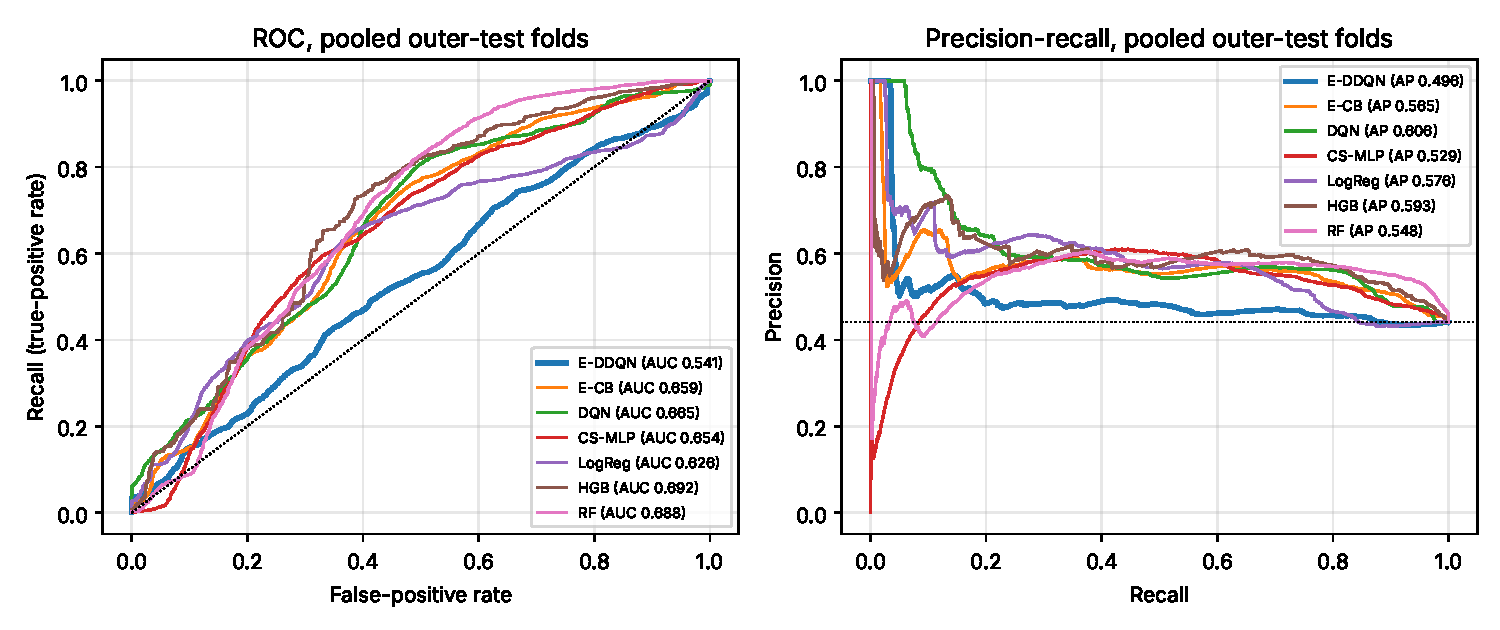
\includegraphics[width=\textwidth]{figs/roc_pr_main.pdf}
\end{center}

\section{Telemetry-perturbation stress tests}
\label{sec:s-attacks}

\subsection{Design (frozen before evaluation; \texttt{configs/\allowbreak attacks.json})}
Perturbations act on the raw per-second channels of the outer-test sessions; causal features are then recomputed with the training-fitted featurizer and scaler of each inner model. Cybersickness labels are never modified; the indicator $z$ marks perturbed seconds. Stress scenarios (each over the whole session or one random 60-s window): frame-rate cap at 72, 60 or 45\,fps; uniform orientation jitter $\pm$0.02, 0.05 or 0.10 per quaternion component; speed up-scaling by 10, 25 or 50\,\% with acceleration recomputed as the per-second speed difference (as in the logger); speed spikes of 10, 20 or 40 units every 20\,s. Evasion-only candidates (whole session): speed down-scaling by 25 or 50\,\%, orientation smoothing with $\lambda=0.5$ or 0.25, frame-rate restoration to 90\,fps. All values are clipped to the per-game ranges observed in the data. Field-of-view manipulation is not evaluated because the field of view never varies in the data.

\subsection{Interpretation limits}
The tests measure how bounded manipulation of the logged channels moves the detectors' scores and decisions. They do not show that a manipulation would cause or hide cybersickness in a person, because no physiological effect was measured. The adaptive worst cases give the adversary the labels and choose the most damaging candidate per session and model.

\subsection{All variants}
Recall and false-positive rate on perturbed seconds (\%) and 5:1 cost on those seconds, clean vs.\ perturbed, seed ensembles at the D1 operating point.

{\scriptsize\setlength{\tabcolsep}{2.5pt}\begin{longtable}{llrlrrrrrr}
\toprule
Model & Scenario & Value & Window & Rec. clean & Rec. att. & FPR clean & FPR att. & Cost clean & Cost att. \\
\midrule
\endhead
CS-MLP & accel spikes & 10 & whole & 99.4 & 99.6 & 93.9 & 95.5 & 0.537 & 0.542 \\
CS-MLP & accel spikes & 10 & window60 & 99.3 & 99.7 & 90.5 & 92.4 & 0.532 & 0.536 \\
CS-MLP & accel spikes & 20 & whole & 99.4 & 99.8 & 93.9 & 98.3 & 0.537 & 0.553 \\
CS-MLP & accel spikes & 20 & window60 & 100.0 & 100.0 & 89.2 & 97.9 & 0.545 & 0.599 \\
CS-MLP & accel spikes & 40 & whole & 99.4 & 99.9 & 93.9 & 99.1 & 0.537 & 0.556 \\
CS-MLP & accel spikes & 40 & window60 & 100.0 & 100.0 & 97.0 & 99.6 & 0.496 & 0.510 \\
CS-MLP & fps cap & 45 & whole & 99.4 & 100.0 & 93.9 & 98.3 & 0.537 & 0.549 \\
CS-MLP & fps cap & 45 & window60 & 99.5 & 100.0 & 95.4 & 98.8 & 0.509 & 0.514 \\
CS-MLP & fps cap & 60 & whole & 99.4 & 100.0 & 93.9 & 98.3 & 0.537 & 0.549 \\
CS-MLP & fps cap & 60 & window60 & 98.6 & 100.0 & 95.4 & 99.0 & 0.649 & 0.649 \\
CS-MLP & fps cap & 72 & whole & 99.4 & 100.0 & 93.9 & 98.3 & 0.537 & 0.549 \\
CS-MLP & fps cap & 72 & window60 & 99.5 & 100.0 & 96.6 & 98.8 & 0.511 & 0.510 \\
CS-MLP & fps restore & 90 & whole & 99.4 & 99.7 & 93.9 & 93.7 & 0.537 & 0.530 \\
CS-MLP & rot jitter & 0.02 & whole & 99.4 & 99.1 & 93.9 & 92.0 & 0.537 & 0.534 \\
CS-MLP & rot jitter & 0.02 & window60 & 99.9 & 99.7 & 96.7 & 94.6 & 0.517 & 0.511 \\
CS-MLP & rot jitter & 0.05 & whole & 99.4 & 98.8 & 93.9 & 91.4 & 0.537 & 0.536 \\
CS-MLP & rot jitter & 0.05 & window60 & 98.3 & 96.4 & 94.4 & 91.2 & 0.656 & 0.667 \\
CS-MLP & rot jitter & 0.1 & whole & 99.4 & 99.7 & 93.9 & 96.5 & 0.537 & 0.545 \\
CS-MLP & rot jitter & 0.1 & window60 & 100.0 & 99.8 & 94.3 & 96.2 & 0.560 & 0.576 \\
CS-MLP & rot smooth & 0.25 & whole & 99.4 & 99.5 & 93.9 & 97.1 & 0.537 & 0.553 \\
CS-MLP & rot smooth & 0.5 & whole & 99.4 & 99.3 & 93.9 & 96.8 & 0.537 & 0.555 \\
CS-MLP & speed scale down & $-$0.5 & whole & 99.4 & 95.6 & 93.9 & 85.3 & 0.537 & 0.573 \\
CS-MLP & speed scale down & $-$0.25 & whole & 99.4 & 98.5 & 93.9 & 90.2 & 0.537 & 0.538 \\
CS-MLP & speed scale up & 0.1 & whole & 99.4 & 99.6 & 93.9 & 95.1 & 0.537 & 0.540 \\
CS-MLP & speed scale up & 0.1 & window60 & 99.3 & 99.7 & 92.2 & 94.1 & 0.541 & 0.544 \\
CS-MLP & speed scale up & 0.25 & whole & 99.4 & 100.0 & 93.9 & 96.7 & 0.537 & 0.541 \\
CS-MLP & speed scale up & 0.25 & window60 & 100.0 & 100.0 & 95.3 & 97.2 & 0.534 & 0.544 \\
CS-MLP & speed scale up & 0.5 & whole & 99.4 & 100.0 & 93.9 & 98.2 & 0.537 & 0.548 \\
CS-MLP & speed scale up & 0.5 & window60 & 100.0 & 100.0 & 87.4 & 97.1 & 0.448 & 0.497 \\
DQN & accel spikes & 10 & whole & 96.9 & 96.8 & 83.7 & 86.1 & 0.536 & 0.552 \\
DQN & accel spikes & 10 & window60 & 92.6 & 92.6 & 80.3 & 82.7 & 0.617 & 0.631 \\
DQN & accel spikes & 20 & whole & 96.9 & 98.3 & 83.7 & 95.5 & 0.536 & 0.570 \\
DQN & accel spikes & 20 & window60 & 96.9 & 97.4 & 78.5 & 98.0 & 0.540 & 0.650 \\
DQN & accel spikes & 40 & whole & 96.9 & 97.9 & 83.7 & 95.4 & 0.536 & 0.578 \\
DQN & accel spikes & 40 & window60 & 99.5 & 100.0 & 87.5 & 99.8 & 0.460 & 0.511 \\
DQN & fps cap & 45 & whole & 96.9 & 96.9 & 83.7 & 83.7 & 0.536 & 0.536 \\
DQN & fps cap & 45 & window60 & 94.1 & 94.1 & 84.5 & 84.5 & 0.581 & 0.581 \\
DQN & fps cap & 60 & whole & 96.9 & 96.9 & 83.7 & 83.7 & 0.536 & 0.536 \\
DQN & fps cap & 60 & window60 & 94.5 & 94.5 & 83.7 & 83.7 & 0.643 & 0.643 \\
DQN & fps cap & 72 & whole & 96.9 & 96.9 & 83.7 & 83.7 & 0.536 & 0.536 \\
DQN & fps cap & 72 & window60 & 93.5 & 93.5 & 83.9 & 83.9 & 0.591 & 0.591 \\
DQN & fps restore & 90 & whole & 96.9 & 96.9 & 83.7 & 83.7 & 0.536 & 0.536 \\
DQN & rot jitter & 0.02 & whole & 96.9 & 94.2 & 83.7 & 78.0 & 0.536 & 0.563 \\
DQN & rot jitter & 0.02 & window60 & 95.6 & 95.5 & 85.1 & 83.4 & 0.555 & 0.548 \\
DQN & rot jitter & 0.05 & whole & 96.9 & 93.2 & 83.7 & 74.7 & 0.536 & 0.568 \\
DQN & rot jitter & 0.05 & window60 & 92.5 & 78.9 & 82.7 & 74.8 & 0.676 & 0.852 \\
DQN & rot jitter & 0.1 & whole & 96.9 & 94.8 & 83.7 & 83.5 & 0.536 & 0.581 \\
DQN & rot jitter & 0.1 & window60 & 96.3 & 95.7 & 86.6 & 84.7 & 0.590 & 0.591 \\
DQN & rot smooth & 0.25 & whole & 96.9 & 99.6 & 83.7 & 92.4 & 0.536 & 0.525 \\
DQN & rot smooth & 0.5 & whole & 96.9 & 98.9 & 83.7 & 91.0 & 0.536 & 0.533 \\
DQN & speed scale down & $-$0.5 & whole & 96.9 & 92.2 & 83.7 & 70.6 & 0.536 & 0.567 \\
DQN & speed scale down & $-$0.25 & whole & 96.9 & 94.7 & 83.7 & 76.9 & 0.536 & 0.547 \\
DQN & speed scale up & 0.1 & whole & 96.9 & 97.0 & 83.7 & 88.1 & 0.536 & 0.557 \\
DQN & speed scale up & 0.1 & window60 & 92.6 & 92.6 & 84.6 & 86.5 & 0.640 & 0.651 \\
DQN & speed scale up & 0.25 & whole & 96.9 & 97.4 & 83.7 & 90.8 & 0.536 & 0.564 \\
DQN & speed scale up & 0.25 & window60 & 97.2 & 97.0 & 82.6 & 87.9 & 0.523 & 0.558 \\
DQN & speed scale up & 0.5 & whole & 96.9 & 97.8 & 83.7 & 91.8 & 0.536 & 0.562 \\
DQN & speed scale up & 0.5 & window60 & 99.5 & 99.5 & 76.4 & 86.4 & 0.403 & 0.455 \\
E-CB & accel spikes & 10 & whole & 96.6 & 97.9 & 85.4 & 88.3 & 0.552 & 0.540 \\
E-CB & accel spikes & 10 & window60 & 97.0 & 98.2 & 77.4 & 79.1 & 0.506 & 0.491 \\
E-CB & accel spikes & 20 & whole & 96.6 & 98.9 & 85.4 & 97.0 & 0.552 & 0.566 \\
E-CB & accel spikes & 20 & window60 & 95.0 & 96.0 & 76.4 & 94.8 & 0.564 & 0.657 \\
E-CB & accel spikes & 40 & whole & 96.6 & 99.3 & 85.4 & 97.7 & 0.552 & 0.562 \\
E-CB & accel spikes & 40 & window60 & 99.5 & 100.0 & 89.4 & 99.3 & 0.469 & 0.508 \\
E-CB & fps cap & 45 & whole & 96.6 & 96.6 & 85.4 & 85.4 & 0.552 & 0.552 \\
E-CB & fps cap & 45 & window60 & 96.0 & 96.0 & 84.2 & 84.2 & 0.533 & 0.533 \\
E-CB & fps cap & 60 & whole & 96.6 & 96.6 & 85.4 & 85.4 & 0.552 & 0.552 \\
E-CB & fps cap & 60 & window60 & 94.6 & 94.6 & 87.2 & 87.2 & 0.663 & 0.663 \\
E-CB & fps cap & 72 & whole & 96.6 & 96.6 & 85.4 & 85.4 & 0.552 & 0.552 \\
E-CB & fps cap & 72 & window60 & 97.0 & 97.0 & 86.2 & 86.2 & 0.518 & 0.518 \\
E-CB & fps restore & 90 & whole & 96.6 & 96.6 & 85.4 & 85.4 & 0.552 & 0.552 \\
E-CB & rot jitter & 0.02 & whole & 96.6 & 96.5 & 85.4 & 76.3 & 0.552 & 0.504 \\
E-CB & rot jitter & 0.02 & window60 & 97.9 & 95.5 & 85.3 & 81.9 & 0.502 & 0.540 \\
E-CB & rot jitter & 0.05 & whole & 96.6 & 94.4 & 85.4 & 79.1 & 0.552 & 0.565 \\
E-CB & rot jitter & 0.05 & window60 & 93.9 & 86.8 & 84.6 & 71.4 & 0.664 & 0.695 \\
E-CB & rot jitter & 0.1 & whole & 96.6 & 96.1 & 85.4 & 88.2 & 0.552 & 0.578 \\
E-CB & rot jitter & 0.1 & window60 & 97.7 & 95.0 & 88.5 & 82.7 & 0.572 & 0.593 \\
E-CB & rot smooth & 0.25 & whole & 96.6 & 95.9 & 85.4 & 94.4 & 0.552 & 0.618 \\
E-CB & rot smooth & 0.5 & whole & 96.6 & 95.3 & 85.4 & 90.9 & 0.552 & 0.612 \\
E-CB & speed scale down & $-$0.5 & whole & 96.6 & 81.0 & 85.4 & 59.5 & 0.552 & 0.752 \\
E-CB & speed scale down & $-$0.25 & whole & 96.6 & 88.9 & 85.4 & 71.2 & 0.552 & 0.643 \\
E-CB & speed scale up & 0.1 & whole & 96.6 & 98.0 & 85.4 & 91.0 & 0.552 & 0.552 \\
E-CB & speed scale up & 0.1 & window60 & 97.4 & 98.2 & 79.4 & 82.2 & 0.509 & 0.508 \\
E-CB & speed scale up & 0.25 & whole & 96.6 & 98.2 & 85.4 & 94.1 & 0.552 & 0.565 \\
E-CB & speed scale up & 0.25 & window60 & 95.6 & 95.4 & 84.8 & 91.4 & 0.572 & 0.614 \\
E-CB & speed scale up & 0.5 & whole & 96.6 & 98.7 & 85.4 & 95.9 & 0.552 & 0.564 \\
E-CB & speed scale up & 0.5 & window60 & 99.1 & 99.5 & 73.3 & 89.3 & 0.397 & 0.469 \\
E-DDQN & accel spikes & 10 & whole & 90.4 & 90.5 & 91.9 & 92.1 & 0.726 & 0.723 \\
E-DDQN & accel spikes & 10 & window60 & 91.7 & 91.4 & 97.9 & 98.0 & 0.737 & 0.745 \\
E-DDQN & accel spikes & 20 & whole & 90.4 & 94.9 & 91.9 & 93.8 & 0.726 & 0.637 \\
E-DDQN & accel spikes & 20 & window60 & 88.8 & 90.4 & 94.5 & 96.0 & 0.796 & 0.774 \\
E-DDQN & accel spikes & 40 & whole & 90.4 & 95.4 & 91.9 & 94.3 & 0.726 & 0.627 \\
E-DDQN & accel spikes & 40 & window60 & 94.0 & 94.0 & 98.7 & 99.9 & 0.651 & 0.657 \\
E-DDQN & fps cap & 45 & whole & 90.4 & 90.4 & 91.9 & 91.9 & 0.726 & 0.726 \\
E-DDQN & fps cap & 45 & window60 & 90.2 & 90.2 & 99.3 & 99.3 & 0.752 & 0.752 \\
E-DDQN & fps cap & 60 & whole & 90.4 & 90.4 & 91.9 & 91.9 & 0.726 & 0.726 \\
E-DDQN & fps cap & 60 & window60 & 83.7 & 83.7 & 95.5 & 95.5 & 0.907 & 0.907 \\
E-DDQN & fps cap & 72 & whole & 90.4 & 90.4 & 91.9 & 91.9 & 0.726 & 0.726 \\
E-DDQN & fps cap & 72 & window60 & 89.1 & 89.1 & 99.2 & 99.2 & 0.775 & 0.775 \\
E-DDQN & fps restore & 90 & whole & 90.4 & 90.4 & 91.9 & 91.9 & 0.726 & 0.726 \\
E-DDQN & rot jitter & 0.02 & whole & 90.4 & 92.7 & 91.9 & 91.4 & 0.726 & 0.671 \\
E-DDQN & rot jitter & 0.02 & window60 & 91.4 & 92.7 & 100.0 & 100.0 & 0.734 & 0.702 \\
E-DDQN & rot jitter & 0.05 & whole & 90.4 & 93.9 & 91.9 & 91.2 & 0.726 & 0.644 \\
E-DDQN & rot jitter & 0.05 & window60 & 83.2 & 82.1 & 88.5 & 88.5 & 0.870 & 0.889 \\
E-DDQN & rot jitter & 0.1 & whole & 90.4 & 94.0 & 91.9 & 92.2 & 0.726 & 0.648 \\
E-DDQN & rot jitter & 0.1 & window60 & 91.0 & 84.7 & 88.5 & 91.4 & 0.708 & 0.854 \\
E-DDQN & rot smooth & 0.25 & whole & 90.4 & 88.0 & 91.9 & 91.8 & 0.726 & 0.777 \\
E-DDQN & rot smooth & 0.5 & whole & 90.4 & 88.9 & 91.9 & 92.3 & 0.726 & 0.760 \\
E-DDQN & speed scale down & $-$0.5 & whole & 90.4 & 86.7 & 91.9 & 90.9 & 0.726 & 0.802 \\
E-DDQN & speed scale down & $-$0.25 & whole & 90.4 & 88.2 & 91.9 & 91.7 & 0.726 & 0.772 \\
E-DDQN & speed scale up & 0.1 & whole & 90.4 & 91.4 & 91.9 & 92.0 & 0.726 & 0.704 \\
E-DDQN & speed scale up & 0.1 & window60 & 91.3 & 92.0 & 98.4 & 98.4 & 0.748 & 0.734 \\
E-DDQN & speed scale up & 0.25 & whole & 90.4 & 92.8 & 91.9 & 91.8 & 0.726 & 0.672 \\
E-DDQN & speed scale up & 0.25 & window60 & 87.0 & 88.3 & 99.8 & 99.9 & 0.845 & 0.817 \\
E-DDQN & speed scale up & 0.5 & whole & 90.4 & 93.5 & 91.9 & 90.7 & 0.726 & 0.650 \\
E-DDQN & speed scale up & 0.5 & window60 & 94.0 & 94.0 & 91.0 & 90.9 & 0.612 & 0.611 \\
HGB & accel spikes & 10 & whole & 97.0 & 97.1 & 85.4 & 87.8 & 0.543 & 0.555 \\
HGB & accel spikes & 10 & window60 & 99.3 & 99.3 & 86.1 & 88.5 & 0.507 & 0.521 \\
HGB & accel spikes & 20 & whole & 97.0 & 97.9 & 85.4 & 94.5 & 0.543 & 0.575 \\
HGB & accel spikes & 20 & window60 & 91.2 & 92.8 & 81.8 & 95.3 & 0.670 & 0.724 \\
HGB & accel spikes & 40 & whole & 97.0 & 98.1 & 85.4 & 95.7 & 0.543 & 0.577 \\
HGB & accel spikes & 40 & window60 & 99.5 & 100.0 & 90.1 & 97.6 & 0.473 & 0.500 \\
HGB & fps cap & 45 & whole & 97.0 & 97.0 & 85.4 & 85.9 & 0.543 & 0.545 \\
HGB & fps cap & 45 & window60 & 93.9 & 93.9 & 89.0 & 89.2 & 0.609 & 0.610 \\
HGB & fps cap & 60 & whole & 97.0 & 97.0 & 85.4 & 85.9 & 0.543 & 0.545 \\
HGB & fps cap & 60 & window60 & 97.5 & 97.5 & 92.3 & 92.4 & 0.648 & 0.649 \\
HGB & fps cap & 72 & whole & 97.0 & 97.0 & 85.4 & 85.9 & 0.543 & 0.545 \\
HGB & fps cap & 72 & window60 & 99.4 & 99.4 & 88.4 & 88.6 & 0.471 & 0.472 \\
HGB & fps restore & 90 & whole & 97.0 & 97.0 & 85.4 & 86.9 & 0.543 & 0.551 \\
HGB & rot jitter & 0.02 & whole & 97.0 & 97.0 & 85.4 & 85.0 & 0.543 & 0.541 \\
HGB & rot jitter & 0.02 & window60 & 99.4 & 99.4 & 87.9 & 87.7 & 0.482 & 0.481 \\
HGB & rot jitter & 0.05 & whole & 97.0 & 96.6 & 85.4 & 82.9 & 0.543 & 0.538 \\
HGB & rot jitter & 0.05 & window60 & 91.6 & 90.2 & 84.6 & 82.0 & 0.703 & 0.710 \\
HGB & rot jitter & 0.1 & whole & 97.0 & 96.3 & 85.4 & 82.7 & 0.543 & 0.543 \\
HGB & rot jitter & 0.1 & window60 & 91.3 & 89.9 & 84.0 & 77.4 & 0.676 & 0.664 \\
HGB & rot smooth & 0.25 & whole & 97.0 & 97.0 & 85.4 & 88.3 & 0.543 & 0.558 \\
HGB & rot smooth & 0.5 & whole & 97.0 & 96.9 & 85.4 & 88.0 & 0.543 & 0.559 \\
HGB & speed scale down & $-$0.5 & whole & 97.0 & 81.0 & 85.4 & 64.4 & 0.543 & 0.780 \\
HGB & speed scale down & $-$0.25 & whole & 97.0 & 91.0 & 85.4 & 78.3 & 0.543 & 0.635 \\
HGB & speed scale up & 0.1 & whole & 97.0 & 97.3 & 85.4 & 88.9 & 0.543 & 0.556 \\
HGB & speed scale up & 0.1 & window60 & 99.4 & 99.4 & 81.9 & 83.3 & 0.479 & 0.487 \\
HGB & speed scale up & 0.25 & whole & 97.0 & 98.0 & 85.4 & 90.7 & 0.543 & 0.550 \\
HGB & speed scale up & 0.25 & window60 & 92.9 & 94.3 & 88.1 & 92.3 & 0.649 & 0.643 \\
HGB & speed scale up & 0.5 & whole & 97.0 & 98.2 & 85.4 & 91.7 & 0.543 & 0.551 \\
HGB & speed scale up & 0.5 & window60 & 99.4 & 99.4 & 77.3 & 87.1 & 0.411 & 0.461 \\
LogReg & accel spikes & 10 & whole & 99.1 & 99.2 & 91.9 & 92.6 & 0.532 & 0.536 \\
LogReg & accel spikes & 10 & window60 & 99.4 & 99.4 & 88.9 & 89.5 & 0.520 & 0.524 \\
LogReg & accel spikes & 20 & whole & 99.1 & 99.3 & 91.9 & 94.8 & 0.532 & 0.545 \\
LogReg & accel spikes & 20 & window60 & 99.4 & 99.4 & 86.4 & 92.6 & 0.540 & 0.578 \\
LogReg & accel spikes & 40 & whole & 99.1 & 99.9 & 91.9 & 96.7 & 0.532 & 0.543 \\
LogReg & accel spikes & 40 & window60 & 99.5 & 99.5 & 89.2 & 93.6 & 0.468 & 0.491 \\
LogReg & fps cap & 45 & whole & 99.1 & 97.0 & 91.9 & 86.3 & 0.532 & 0.549 \\
LogReg & fps cap & 45 & window60 & 99.5 & 86.8 & 93.0 & 82.4 & 0.496 & 0.745 \\
LogReg & fps cap & 60 & whole & 99.1 & 98.1 & 91.9 & 88.4 & 0.532 & 0.535 \\
LogReg & fps cap & 60 & window60 & 99.3 & 89.7 & 92.4 & 84.3 & 0.618 & 0.729 \\
LogReg & fps cap & 72 & whole & 99.1 & 98.6 & 91.9 & 90.2 & 0.532 & 0.534 \\
LogReg & fps cap & 72 & window60 & 99.5 & 95.2 & 91.7 & 88.3 & 0.486 & 0.573 \\
LogReg & fps restore & 90 & whole & 99.1 & 99.1 & 91.9 & 91.9 & 0.532 & 0.532 \\
LogReg & rot jitter & 0.02 & whole & 99.1 & 99.2 & 91.9 & 92.1 & 0.532 & 0.533 \\
LogReg & rot jitter & 0.02 & window60 & 99.5 & 99.5 & 91.5 & 91.6 & 0.499 & 0.500 \\
LogReg & rot jitter & 0.05 & whole & 99.1 & 99.3 & 91.9 & 92.5 & 0.532 & 0.533 \\
LogReg & rot jitter & 0.05 & window60 & 96.4 & 96.8 & 92.2 & 92.5 & 0.673 & 0.668 \\
LogReg & rot jitter & 0.1 & whole & 99.1 & 99.2 & 91.9 & 92.7 & 0.532 & 0.535 \\
LogReg & rot jitter & 0.1 & window60 & 95.7 & 96.9 & 91.1 & 91.3 & 0.629 & 0.605 \\
LogReg & rot smooth & 0.25 & whole & 99.1 & 99.1 & 91.9 & 91.7 & 0.532 & 0.532 \\
LogReg & rot smooth & 0.5 & whole & 99.1 & 99.1 & 91.9 & 91.7 & 0.532 & 0.532 \\
LogReg & speed scale down & $-$0.5 & whole & 99.1 & 97.8 & 91.9 & 86.8 & 0.532 & 0.534 \\
LogReg & speed scale down & $-$0.25 & whole & 99.1 & 98.7 & 91.9 & 89.2 & 0.532 & 0.526 \\
LogReg & speed scale up & 0.1 & whole & 99.1 & 99.2 & 91.9 & 92.9 & 0.532 & 0.536 \\
LogReg & speed scale up & 0.1 & window60 & 99.4 & 99.4 & 87.8 & 88.7 & 0.513 & 0.518 \\
LogReg & speed scale up & 0.25 & whole & 99.1 & 99.4 & 91.9 & 93.6 & 0.532 & 0.536 \\
LogReg & speed scale up & 0.25 & window60 & 99.4 & 99.4 & 90.8 & 91.9 & 0.520 & 0.527 \\
LogReg & speed scale up & 0.5 & whole & 99.1 & 99.7 & 91.9 & 94.9 & 0.532 & 0.537 \\
LogReg & speed scale up & 0.5 & window60 & 99.5 & 99.5 & 86.0 & 92.5 & 0.452 & 0.486 \\
RF & accel spikes & 10 & whole & 98.7 & 99.0 & 81.7 & 84.5 & 0.485 & 0.494 \\
RF & accel spikes & 10 & window60 & 99.3 & 99.3 & 75.0 & 79.1 & 0.444 & 0.467 \\
RF & accel spikes & 20 & whole & 98.7 & 99.7 & 81.7 & 96.2 & 0.485 & 0.543 \\
RF & accel spikes & 20 & window60 & 97.6 & 99.1 & 68.6 & 96.2 & 0.466 & 0.605 \\
RF & accel spikes & 40 & whole & 98.7 & 99.8 & 81.7 & 97.4 & 0.485 & 0.549 \\
RF & accel spikes & 40 & window60 & 99.5 & 100.0 & 81.1 & 99.8 & 0.427 & 0.511 \\
RF & fps cap & 45 & whole & 98.7 & 98.7 & 81.7 & 81.3 & 0.485 & 0.483 \\
RF & fps cap & 45 & window60 & 99.4 & 99.4 & 84.9 & 84.9 & 0.456 & 0.456 \\
RF & fps cap & 60 & whole & 98.7 & 98.7 & 81.7 & 81.3 & 0.485 & 0.483 \\
RF & fps cap & 60 & window60 & 99.2 & 99.2 & 84.7 & 84.7 & 0.569 & 0.569 \\
RF & fps cap & 72 & whole & 98.7 & 98.7 & 81.7 & 81.3 & 0.485 & 0.483 \\
RF & fps cap & 72 & window60 & 99.4 & 99.4 & 85.6 & 85.6 & 0.457 & 0.457 \\
RF & fps restore & 90 & whole & 98.7 & 98.8 & 81.7 & 81.8 & 0.485 & 0.483 \\
RF & rot jitter & 0.02 & whole & 98.7 & 98.2 & 81.7 & 79.4 & 0.485 & 0.482 \\
RF & rot jitter & 0.02 & window60 & 99.4 & 99.4 & 85.0 & 83.0 & 0.467 & 0.456 \\
RF & rot jitter & 0.05 & whole & 98.7 & 97.7 & 81.7 & 79.0 & 0.485 & 0.491 \\
RF & rot jitter & 0.05 & window60 & 96.1 & 91.5 & 84.3 & 82.4 & 0.625 & 0.691 \\
RF & rot jitter & 0.1 & whole & 98.7 & 98.0 & 81.7 & 81.1 & 0.485 & 0.496 \\
RF & rot jitter & 0.1 & window60 & 96.3 & 92.8 & 82.1 & 79.1 & 0.563 & 0.616 \\
RF & rot smooth & 0.25 & whole & 98.7 & 99.0 & 81.7 & 85.9 & 0.485 & 0.502 \\
RF & rot smooth & 0.5 & whole & 98.7 & 99.1 & 81.7 & 84.9 & 0.485 & 0.494 \\
RF & speed scale down & $-$0.5 & whole & 98.7 & 90.6 & 81.7 & 61.8 & 0.485 & 0.553 \\
RF & speed scale down & $-$0.25 & whole & 98.7 & 95.9 & 81.7 & 73.3 & 0.485 & 0.501 \\
RF & speed scale up & 0.1 & whole & 98.7 & 99.1 & 81.7 & 84.3 & 0.485 & 0.492 \\
RF & speed scale up & 0.1 & window60 & 99.0 & 99.0 & 75.5 & 77.5 & 0.452 & 0.464 \\
RF & speed scale up & 0.25 & whole & 98.7 & 99.1 & 81.7 & 86.7 & 0.485 & 0.504 \\
RF & speed scale up & 0.25 & window60 & 98.6 & 98.3 & 84.0 & 85.5 & 0.502 & 0.515 \\
RF & speed scale up & 0.5 & whole & 98.7 & 99.0 & 81.7 & 92.1 & 0.485 & 0.537 \\
RF & speed scale up & 0.5 & window60 & 99.4 & 99.4 & 66.3 & 85.6 & 0.354 & 0.453 \\
\bottomrule
\end{longtable}
}

\section{Post-hoc analyses}
\label{sec:s-posthoc}
The analyses in this section were specified after the primary results were known, committed (\texttt{configs/\allowbreak posthoc.json}) before they were run, and use the splits, inner folds, selection objective, checkpoint and threshold rules, cross-fitting recipe and final seeds of the primary protocol. No primary result was changed. Sections~S5.7--S5.9 were added after a pre-submission review, when all other results were known (\texttt{configs/\allowbreak posthoc.json}, key \texttt{review\_round\_2}); they use only the saved per-sample predictions and selected configurations.

\subsection{Exposure-time baselines: selected configurations}
Time-LR searched all six values of $C$; Time+game HGB used the HGB search space and budget (16 configurations).

\begin{center}\footnotesize
\begin{tabular}{lcllc}
\toprule
Model & Outer fold & Feature set & Selected hyper-parameters & Inner-OOF cost \\
\midrule
Time-LR & 0 & time & C = 0.001 & 0.471 \\
Time-LR & 1 & time & C = 1 & 0.528 \\
Time-LR & 2 & time & C = 0.1 & 0.549 \\
Time-LR & 3 & time & C = 0.01 & 0.497 \\
Time-LR & 4 & time & C = 0.1 & 0.550 \\
Time+game HGB & 0 & time+game & lr 0.02, iter 200, leaves 8, min leaf 300, $\ell_2$ 1 & 0.480 \\
Time+game HGB & 1 & time+game & lr 0.02, iter 200, leaves 8, min leaf 300, $\ell_2$ 0 & 0.501 \\
Time+game HGB & 2 & time+game & lr 0.02, iter 100, leaves 4, min leaf 300, $\ell_2$ 10 & 0.524 \\
Time+game HGB & 3 & time+game & lr 0.02, iter 200, leaves 4, min leaf 300, $\ell_2$ 1 & 0.522 \\
Time+game HGB & 4 & time+game & lr 0.02, iter 200, leaves 8, min leaf 300, $\ell_2$ 0 & 0.506 \\
\bottomrule
\end{tabular}

\end{center}

\subsection{Holm adjustment of the paired comparisons}
Group-bootstrap comparisons of E-DDQN with the six other primary models under each operating rule, with Holm's step-down adjustment over the six comparisons of each rule.

\begin{center}\footnotesize
\begin{tabular}{llcccc}
\toprule
Rule & B & $\Delta$Cost (E-DDQN$-$B) & 95\,\% CI & $p_{\text{group}}$ & $p_{\text{Holm}}$ \\
\midrule
D1 (min cost) & E-CB & +0.175 & [+0.016, +0.448] & 0.014 & 0.070 \\
D1 (min cost) & DQN & +0.190 & [$-$0.017, +0.493] & 0.079 & 0.105 \\
D1 (min cost) & CS-MLP & +0.190 & [+0.005, +0.485] & 0.039 & 0.105 \\
D1 (min cost) & LogReg & +0.194 & [+0.011, +0.477] & 0.026 & 0.104 \\
D1 (min cost) & HGB & +0.183 & [+0.011, +0.460] & 0.035 & 0.105 \\
D1 (min cost) & RF & +0.242 & [+0.052, +0.528] & 0.001 & 0.006 \\
D0 ($\hat p\ge1/6$) & E-CB & +0.214 & [+0.025, +0.487] & 0.018 & 0.054 \\
D0 ($\hat p\ge1/6$) & DQN & +0.242 & [+0.039, +0.542] & 0.012 & 0.048 \\
D0 ($\hat p\ge1/6$) & CS-MLP & +0.204 & [$-$0.030, +0.507] & 0.113 & 0.226 \\
D0 ($\hat p\ge1/6$) & LogReg & +0.087 & [$-$0.293, +0.541] & 0.694 & 0.694 \\
D0 ($\hat p\ge1/6$) & HGB & +0.328 & [+0.078, +0.639] & 0.003 & 0.015 \\
D0 ($\hat p\ge1/6$) & RF & +0.411 & [+0.147, +0.748] & 0.001 & 0.006 \\
val.\ recall $\ge$0.95 & E-CB & +0.220 & [+0.017, +0.566] & 0.021 & 0.080 \\
val.\ recall $\ge$0.95 & DQN & +0.236 & [+0.013, +0.580] & 0.028 & 0.080 \\
val.\ recall $\ge$0.95 & CS-MLP & +0.294 & [+0.033, +0.652] & 0.013 & 0.065 \\
val.\ recall $\ge$0.95 & LogReg & +0.307 & [+0.027, +0.687] & 0.020 & 0.080 \\
val.\ recall $\ge$0.95 & HGB & +0.314 & [+0.030, +0.711] & 0.023 & 0.080 \\
val.\ recall $\ge$0.95 & RF & +0.342 & [+0.067, +0.719] & 0.003 & 0.018 \\
\bottomrule
\end{tabular}

\end{center}

\subsection{Comparison with always alarming}
Paired bootstrap of each model's D1 cost (seed ensemble) minus the cost of always alarming; Holm adjustment over the nine models (group units).

\begin{center}\footnotesize
\resizebox{\textwidth}{!}{\begin{tabular}{lcccccc}
\toprule
Model & $\Delta$Cost (model$-$always) & CI (groups) & $p$ & $p_{\text{Holm}}$ & CI (sessions) & $p$ \\
\midrule
E-DDQN & +0.168 & [$-$0.024, +0.466] & 0.104 & 0.728 & [$-$0.026, +0.438] & 0.116 \\
E-CB & $-$0.007 & [$-$0.093, +0.103] & 0.810 & 1.000 & [$-$0.089, +0.105] & 0.800 \\
DQN & $-$0.022 & [$-$0.104, +0.062] & 0.560 & 1.000 & [$-$0.099, +0.075] & 0.598 \\
CS-MLP & $-$0.022 & [$-$0.046, $-$0.002] & 0.037 & 0.296 & [$-$0.049, +0.004] & 0.109 \\
LogReg & $-$0.026 & [$-$0.061, +0.006] & 0.136 & 0.816 & [$-$0.058, +0.005] & 0.113 \\
HGB & $-$0.015 & [$-$0.122, +0.121] & 0.765 & 1.000 & [$-$0.104, +0.092] & 0.744 \\
RF & $-$0.074 & [$-$0.135, $-$0.019] & 0.012 & 0.108 & [$-$0.120, $-$0.025] & 0.002 \\
Time-LR & $-$0.010 & [$-$0.073, +0.080] & 0.737 & 1.000 & [$-$0.080, +0.080] & 0.782 \\
Time+game HGB & $-$0.041 & [$-$0.100, +0.051] & 0.302 & 1.000 & [$-$0.099, +0.048] & 0.275 \\
\bottomrule
\end{tabular}
}
\end{center}

\subsection{Grouping sensitivity}
Paired bootstrap resampling sessions instead of linkage groups (Holm over the six primary comparisons), and the range of the cost difference in a leave-one-group-out jackknife over the \nGroupsEval{} groups.

\begin{center}\footnotesize
\resizebox{\textwidth}{!}{\begin{tabular}{lcccccc}
\toprule
B & $\Delta$Cost (E-DDQN$-$B) & CI (sessions) & $p$ & $p_{\text{Holm}}$ & jackknife range & sign flips \\
\midrule
E-CB & +0.175 & [+0.014, +0.423] & 0.014 & 0.070 & +0.068 to +0.201 & 0 \\
DQN & +0.190 & [+0.001, +0.454] & 0.050 & 0.087 & +0.084 to +0.248 & 0 \\
CS-MLP & +0.190 & [+0.006, +0.452] & 0.037 & 0.087 & +0.084 to +0.225 & 0 \\
LogReg & +0.194 & [+0.007, +0.454] & 0.029 & 0.087 & +0.094 to +0.225 & 0 \\
HGB & +0.183 & [+0.014, +0.440] & 0.021 & 0.084 & +0.076 to +0.215 & 0 \\
RF & +0.242 & [+0.055, +0.503] & 0.001 & 0.006 & +0.137 to +0.284 & 0 \\
Time-LR & +0.178 & [$-$0.015, +0.439] & 0.089 & -- & +0.075 to +0.213 & 0 \\
Time+game HGB & +0.209 & [+0.016, +0.470] & 0.030 & -- & +0.101 to +0.248 & 0 \\
\bottomrule
\end{tabular}
}
\end{center}

\subsection{Validation-chosen cost curves}
Test cost of the seed ensemble divided by the cost of the better trivial policy, for each false-negative to false-positive ratio $R$ (threshold chosen on inner-validation predictions at each $R$). At $R=5$ the values reproduce the D1 seed-ensemble costs exactly (checked programmatically).

\begin{center}\footnotesize
\resizebox{\textwidth}{!}{\begin{tabular}{lcccccccccc}
\toprule
Model & 1 & 1.5 & 2 & 3 & 4 & 5 & 7 & 10 & 15 & 20 \\
\midrule
E-DDQN & 1.004 & 0.921 & 1.034 & 1.130 & 1.241 & 1.301 & 1.382 & 1.322 & 1.448 & 1.508 \\
E-CB & 0.828 & 0.819 & 0.900 & 0.920 & 0.954 & 0.988 & 1.068 & 0.992 & 1.007 & 1.013 \\
DQN & 0.921 & 0.796 & 0.865 & 0.845 & 0.929 & 0.961 & 1.013 & 1.068 & 1.208 & 1.304 \\
CS-MLP & 0.846 & 0.773 & 0.835 & 0.980 & 0.960 & 0.961 & 0.969 & 0.981 & 0.985 & 0.985 \\
LogReg & 0.852 & 0.868 & 0.915 & 0.941 & 0.946 & 0.953 & 0.966 & 0.983 & 0.989 & 1.010 \\
HGB & 0.897 & 0.770 & 0.808 & 0.884 & 0.945 & 0.973 & 1.001 & 0.980 & 0.991 & 0.998 \\
RF & 0.861 & 0.717 & 0.773 & 0.836 & 0.864 & 0.868 & 0.893 & 0.928 & 0.960 & 0.983 \\
Time-LR & 0.843 & 0.718 & 0.781 & 0.840 & 0.883 & 0.982 & 0.990 & 0.984 & 1.000 & 1.000 \\
Time+game HGB & 0.816 & 0.731 & 0.760 & 0.833 & 0.882 & 0.926 & 0.942 & 1.014 & 1.053 & 1.064 \\
\bottomrule
\end{tabular}
}
\end{center}

\subsection{Q-value scale}
Largest absolute Q-value over the final runs of each outer fold relative to the return bound $r_{\max}/(1-\gamma)$ of the selected discount ($r_{\max}=0.5$ for the asymmetric reward, 1 for the symmetric reward).

\begin{center}\footnotesize
\begin{tabular}{lccccc}
\toprule
Model & Outer fold & $\gamma$ & max $|Q|$ & bound $r_{\max}/(1-\gamma)$ & ratio \\
\midrule
E-DDQN & 0 & 0.99 & 41.45 & 50.00 & 0.83 \\
E-DDQN & 1 & 0.99 & 61.78 & 50.00 & 1.24 \\
E-DDQN & 2 & 0.99 & 35.08 & 50.00 & 0.70 \\
E-DDQN & 3 & 0.99 & 4.13 & 50.00 & 0.08 \\
E-DDQN & 4 & 0.9 & 11.56 & 5.00 & 2.31 \\
E-CB & 0 & 0 & 0.70 & 0.50 & 1.41 \\
E-CB & 1 & 0 & 0.68 & 0.50 & 1.37 \\
E-CB & 2 & 0 & 0.68 & 0.50 & 1.36 \\
E-CB & 3 & 0 & 0.89 & 0.50 & 1.79 \\
E-CB & 4 & 0 & 0.95 & 0.50 & 1.89 \\
DQN & 0 & 0 & 2.24 & 1.00 & 2.24 \\
DQN & 1 & 0.9 & 4.09 & 10.00 & 0.41 \\
DQN & 2 & 0.9 & 3.05 & 10.00 & 0.30 \\
DQN & 3 & 0.9 & 10.10 & 10.00 & 1.01 \\
DQN & 4 & 0 & 2.08 & 1.00 & 2.08 \\
\bottomrule
\end{tabular}

\end{center}

\subsection{Within-fold ROC-AUC}
Pooled ROC-AUC combines the test scores of five fold-specific models and therefore mixes discrimination with differences in score scale between folds. Within-fold ROC-AUC is computed in each outer-test fold and averaged over folds (seed mean: also averaged over the five seeds).

\begin{center}\footnotesize
\begin{tabular}{lcccc}
\toprule
Model & Pooled (seed mean) & Within-fold (seed mean) & Pooled (ensemble) & Within-fold (ensemble) \\
\midrule
E-DDQN & 0.538 & 0.539 & 0.541 & 0.552 \\
E-CB & 0.653 & 0.658 & 0.659 & 0.665 \\
DQN & 0.661 & 0.666 & 0.665 & 0.666 \\
CS-MLP & 0.644 & 0.666 & 0.654 & 0.672 \\
LogReg & 0.626 & 0.636 & 0.626 & 0.636 \\
HGB & 0.692 & 0.702 & 0.692 & 0.702 \\
RF & 0.688 & 0.715 & 0.688 & 0.715 \\
Time-LR & 0.704 & 0.709 & 0.704 & 0.709 \\
Time+game HGB & 0.676 & 0.699 & 0.676 & 0.699 \\
\bottomrule
\end{tabular}

\end{center}

\subsection{Exact group sign-flip tests}
Two-sided sign-flip permutation test of the pooled D1 cost difference of the seed ensembles, with the \nGroupsEval{} linkage groups as units and all $2^{21}$ sign patterns enumerated. Holm adjustment over the six primary comparisons with E-DDQN and over the nine comparisons with always alarming. The group-bootstrap $p$-values of Section~S5.2 (rule D1) are shown for comparison.

\begin{center}\footnotesize
\resizebox{\textwidth}{!}{\begin{tabular}{lccccc}
\toprule
Comparison (D1, seed ensembles) & $\Delta$Cost & $p_{\text{boot}}$ & $p_{\text{boot,Holm}}$ & $p_{\text{sign-flip}}$ & $p_{\text{sign-flip,Holm}}$ \\
\midrule
E-DDQN vs E-CB & +0.175 & 0.014 & 0.070 & 0.048 & 0.241 \\
E-DDQN vs DQN & +0.190 & 0.079 & 0.105 & 0.127 & 0.330 \\
E-DDQN vs CS-MLP & +0.190 & 0.039 & 0.105 & 0.116 & 0.330 \\
E-DDQN vs LogReg & +0.194 & 0.026 & 0.104 & 0.094 & 0.330 \\
E-DDQN vs HGB & +0.183 & 0.035 & 0.105 & 0.083 & 0.330 \\
E-DDQN vs RF & +0.242 & 0.001 & 0.006 & 0.014 & 0.083 \\
E-DDQN vs Time-LR & +0.178 & -- & -- & 0.117 & -- \\
E-DDQN vs Time+game HGB & +0.209 & -- & -- & 0.067 & -- \\
E-DDQN vs always alarm & +0.168 &  &  & 0.250 & 1.000 \\
E-CB vs always alarm & $-$0.007 &  &  & 0.922 & 1.000 \\
DQN vs always alarm & $-$0.022 &  &  & 0.620 & 1.000 \\
CS-MLP vs always alarm & $-$0.022 &  &  & 0.053 & 0.422 \\
LogReg vs always alarm & $-$0.026 &  &  & 0.172 & 1.000 \\
HGB vs always alarm & $-$0.015 &  &  & 0.769 & 1.000 \\
RF vs always alarm & $-$0.074 &  &  & 0.022 & 0.194 \\
Time-LR vs always alarm & $-$0.010 &  &  & 0.820 & 1.000 \\
Time+game HGB vs always alarm & $-$0.041 &  &  & 0.358 & 1.000 \\
\bottomrule
\end{tabular}
}
\end{center}

\subsection{Selected feature sets and within-fold ROC-AUC}
Exploratory. Feature set selected on validation data for each primary model and outer fold (T: telemetry; T+Q: telemetry and questionnaire indicators; E: exposure; E+Q: exposure and questionnaire indicators) and the within-fold ROC-AUC of that model on the fold's test groups (mean over seeds). Feature sets were selected, not assigned, so the association does not establish a cause.

\begin{center}\footnotesize
\begin{tabular}{lccccc}
\toprule
Model & Fold 0 & Fold 1 & Fold 2 & Fold 3 & Fold 4 \\
\midrule
E-DDQN & E+Q 0.541 & E+Q 0.505 & E+Q 0.723 & E+Q 0.450 & E+Q 0.476 \\
E-CB & E 0.642 & E 0.717 & E 0.748 & E 0.737 & E+Q 0.446 \\
DQN & E 0.706 & E+Q 0.530 & E 0.843 & E 0.736 & E+Q 0.515 \\
CS-MLP & E+Q 0.562 & E+Q 0.607 & E 0.812 & T 0.702 & T 0.644 \\
LogReg & E 0.623 & T+Q 0.428 & E 0.810 & E 0.712 & E+Q 0.610 \\
HGB & E 0.631 & E 0.740 & E 0.791 & T 0.761 & E 0.585 \\
RF & T 0.630 & E 0.728 & E 0.771 & E 0.761 & T+Q 0.683 \\
\bottomrule
\end{tabular}

\end{center}


\section{Reconstruction of the earlier protocol}
\label{sec:s-earlier}
An earlier, unpublished version of this study reported 96.88\,\% accuracy and 99.53\,\% recall for E-DDQN. Its 41-feature input files, preprocessing code and trained models were not available, so the following is a reconstruction of its protocol, not an exact reproduction. The earlier version's partition sizes (14,680 / 3,146 / 3,146; 20,972 in total; 3,670 training samples per grade) are reproduced exactly by oversampling every discomfort grade of the curated release to the size of grade 0 (5,243) and then splitting at row level.

\noindent\resizebox{\textwidth}{!}{\begin{tabular}{llccccc}
\toprule
Model & Evaluation protocol & Acc. & Recall & Spec. & MCC & ROC-AUC \\
\midrule
HGB & Oversample to 5,243/grade, then 70/15/15 row split (earlier protocol) & 97.6 & 99.8 & 91.0 & 0.935 & 0.995 \\
HGB & Row-level random split, no oversampling & 95.3 & 94.1 & 96.3 & 0.905 & 0.992 \\
HGB & Grouped 5-fold split (session-linkage groups) & 52.2 & 33.6 & 66.9 & 0.005 & 0.523 \\
E-DDQN (earlier code) & Earlier script, earlier protocol (proxy) & 95.2 & 99.2 & 83.1 & 0.870 & -- \\
E-DDQN (earlier code) & Earlier script, grouped split (proxy) & 41.1 & 92.1 & 7.7 & $-$0.004 & -- \\
\bottomrule
\end{tabular}
}

\medskip
Under this protocol \LeakDupPos{} of the \LeakTestPos{} positive test rows (\LeakDupPct\,\%) have an exact duplicate in the training split, and all sessions occur in both splits.

\subsection*{Implementation pitfalls found in the earlier code}
The following defects of the earlier E-DDQN implementation are listed because they are easy to make whenever a classifier is trained as a Q-learner. Items 1--3 are guarded against by the unit tests of the present code (Section~\ref{sec:s-repro}); items 4--6 are avoided by design (the Double-DQN arg-max is computed in evaluation mode, the outer-test data are scored only once after training, and SHAP explains the decision margin $\Delta Q$ rather than $Q(s,1)$ on 400 test rows of each fold, with DeepExplainer and its additivity check tried first and expected gradients used when that check failed, as it did in every fold; main text, Sections~III-E, III-G and III-I).
\begin{enumerate}
\item The next state was the next row of a shuffled chunk, with no terminal flags, so $\gamma=0.99$ bootstrapped across unrelated samples.
\item The true label was stored as the action together with the reward of the random action actually taken (a form of teacher forcing).
\item The Polyak update ignored batch-normalization buffers, so the target network normalized with mean 0 and variance 1 throughout training.
\item The Double-DQN arg-max ran the online network in training mode.
\item The test set was scored during training (every 10 episodes), which invites test-set monitoring.
\item SHAP attributed $Q(s,1)$, which contains $V(s)$, on 50 test rows with the additivity check disabled.
\end{enumerate}

\section{Reproducibility}
\label{sec:s-repro}
\begin{itemize}
\item Software: Python 3.13.16, PyTorch 2.14.1 (CPU), scikit-learn 1.9.1, NumPy 2.5.3, pandas 3.0.5, SciPy 1.18.1, SHAP 0.53.0, statsmodels 0.15.0 (\texttt{requirements.txt}).
\item One command regenerates everything from the raw XML files: \texttt{bash run\_all.sh -{}-fresh} (about 2.5 to 3.5 hours of wall time on four CPU cores, dominated by the reinforcement-learning hyper-parameter searches and ablation). A clean rerun of the final version (commit \texttt{2e49e93}, which differs from this version only in these reproducibility statements) from an empty directory, including the search-draw analysis, took about 2 hours 46 minutes of computing and reproduced every per-sample prediction, every reported number and the text of the paper and supplement exactly; it was interrupted once by a restart of the computing container and resumed from its saved per-job outputs, as recorded in \texttt{results/\allowbreak qc/\allowbreak clean\_rerun.md}.
\item The post-hoc analyses (Section~\ref{sec:s-posthoc}) are recorded in \texttt{configs/\allowbreak posthoc.json}; Section~\ref{sec:s-posthoc} states which of them were committed before they were run and which were added later. They are produced by \texttt{scripts/\allowbreak 11\_posthoc.py} (\texttt{run} and \texttt{analyze}; seeds 801--802 for the post-hoc search, bootstrap seeds 5--7), except the search-draw sensitivity analysis (Section~S5.11, key \texttt{search\_draw\_sensitivity}), which is produced by \texttt{scripts/\allowbreak 13\_search\_draw\_sensitivity.py} (configuration seeds 9120, 9130, 9122, 9132, 9200 and 9202; bootstrap seeds 5 and 6).
\item Seeds: split 20261012 (outer) and 20261013--20261017 (inner); hyper-parameter search 777 (+family index for configuration sampling); final training 1000--1004; perturbations 4242; bootstrap 11 (CIs) and 5 (paired tests).
\item Every number in the manuscript and in this supplement is produced by \texttt{scripts/\allowbreak 05\_make\_tables.py} (primary analysis) from \texttt{results/\allowbreak tables/\allowbreak *.csv}, which \texttt{scripts/\allowbreak 04\_aggregate.py} computes from the per-sample predictions in \texttt{results/\allowbreak predictions/\allowbreak }, or by \texttt{scripts/\allowbreak 11\_posthoc.py} and \texttt{scripts/\allowbreak 13\_search\_draw\_sensitivity.py} (post-hoc analyses, Section~\ref{sec:s-posthoc}). \texttt{scripts/\allowbreak 08\_consistency\_check.py} recomputes confusion matrices, metrics and McNemar statistics with independent library implementations and checks them against the manuscript macros.
\item Executable sanity tests of the corrected agent: \texttt{scripts/\allowbreak 00\_sanity\_tests.py} (reward regret ratio, implied threshold, within-session transitions, terminal flags, reward/action consistency of replay, target-network buffer synchronisation, Q-value bounds, McNemar identity).
\end{itemize}


\end{document}
